%
% Main document
% ===========================================================================
% This is part of the document "Smartwatches in siot.net".
% Authors: paras1
%

% Document informations
%---------------------------------------------------------------------------
\def \module		{Bachelor Thesis}					% Module name
\def \title			{Smartwatches in siot.net}		% Title
\def \version		{X1.0}
\def \author		{Sathesh Paramasamy}
\def \logo			{BFH_Logo_C_de_fr_en_100_4CU}	% choose the correct logo in
													% the folder Bilder/BFH_Logo
%-----------------------------------------------------------------%----------

%---------------------------------------------------------------------------
\documentclass[
	a4paper,				% paper format
	10pt,					% fontsize
%	twoside,				% double-sided
	oneside,				% one-sided
	openright,				% begin new chapter on right side
	notitlepage,			% use no standard title page
	parskip=half,			% set paragraph skip to half of a line
]{scrreprt}					% KOMA-script report
%---------------------------------------------------------------------------

\raggedbottom
\KOMAoptions{cleardoublepage=plain}	% Add header and footer on blank pages


% Load Standard Packages:
%---------------------------------------------------------------------------
\usepackage[standard-baselineskips]{cmbright}

\usepackage[ngerman]{babel}		% german hyphenation
%\usepackage[latin1]{inputenc}  % Unix/Linux - load extended character set (ISO 8859-1)
%\usepackage[ansinew]{inputenc}  % Windows - load extended character set (ISO 8859-1)
\usepackage[utf8]{inputenc}    % UTF-8 - load extended charater set
\usepackage[T1]{fontenc}		% hyphenation of words with ä,ö and ü
\usepackage{textcomp}			% additional symbols
\usepackage{ae}					% better resolution of Type1-Fonts
\usepackage{fancyhdr}			% simple manipulation of header and footer
\usepackage{graphicx}			% integration of images
\usepackage{float}				% floating objects
\usepackage[font=small]{caption}			% for captions of figures and tables
\usepackage{booktabs}			% package for nicer tables
\usepackage{tocvsec2}			% provides means of controlling the sectional numbering
\usepackage{rotating}			% rotating tables and other objects
\usepackage{pdflscape}			% change single pages landscape
\usepackage{tabularx}			% create nice tables
\usepackage{pdfpages}			% insert full pdf pages
\usepackage{nameref}			% reference by name, not by chapter number
\usepackage{dirtree}			% create directory trees
\usepackage{listings}			% include source code
\usepackage{epstopdf}			% convert eps graphics to pdf
\usepackage{colortbl}
%---------------------------------------------------------------------------

% Load Math Packages
%---------------------------------------------------------------------------
\usepackage{amsmath}			% various features to facilitate writing math formulas
\usepackage{amsthm}				% enhanced version of latex's newtheorem
\usepackage{amsfonts}			% set of miscellaneous TeX fonts that augment the standard CM
\usepackage{amssymb}			% mathematical special characters
\usepackage{exscale}			% mathematical size corresponds to textsize
%---------------------------------------------------------------------------

% Package to facilitate placement of boxes at absolute positions
%---------------------------------------------------------------------------
\usepackage[absolute]{textpos}
\setlength{\TPHorizModule}{1mm}
\setlength{\TPVertModule}{1mm}
%---------------------------------------------------------------------------

% Definition of Colors
%---------------------------------------------------------------------------
\RequirePackage{color}							% Color (not xcolor!)
\definecolor{linkblue}{rgb}{0,0,0.8}				% Standard
\definecolor{darkblue}{rgb}{0,0.08,0.45}			% Dark blue
\definecolor{brickred}{cmyk}{0,0.89,0.94,0.28}	% Brickred
\definecolor{bfhred}{rgb}{0.776,0,0.066}			% Red
% specific colors
\definecolor{titlecolor}{rgb}{0,0.08,0.45}		% Color used for the title
%\definecolor{linkcolor}{rgb}{0,0,0.8}			% Blue for the web- and cd-version!
\definecolor{linkcolor}{rgb}{0,0,0}				% Black for the print-version!
\definecolor{code_bg}{gray}{0.8}					% Source Code Background
%---------------------------------------------------------------------------

% Hyperref Package (Create links in a pdf)
%---------------------------------------------------------------------------
\usepackage[
	pdftex,ngerman,bookmarks,plainpages=false,pdfpagelabels,
	backref = {false},					% No index backreference
	colorlinks = {true},					% Color links in a PDF
	hypertexnames = {true},				% no failures "same page(i)"
	bookmarksopen = {true},				% opens the bar on the left side
	bookmarksopenlevel = {0},			% depth of opened bookmarks
	pdftitle = {\title},					% PDF-property
	pdfauthor = {\author},				% PDF-property
	pdfsubject = {\module},				% PDF-property
	linkcolor = {linkcolor},				% Color of Links
	citecolor = {linkcolor},				% Color of Cite-Links
	urlcolor = {linkcolor},				% Color of URLs
]{hyperref}
%---------------------------------------------------------------------------

% Set up page dimension
%---------------------------------------------------------------------------
\usepackage{geometry}
\geometry{
	a4paper,
	left=20mm,
	right=15mm,
	top=30mm,
	headheight=20mm,
	headsep=10mm,
	textheight=232mm,
	footskip=15mm
}
%---------------------------------------------------------------------------

% Makeindex Package
%---------------------------------------------------------------------------
\usepackage{makeidx}				% To produce index
\makeindex						% Index-Initialisation
%---------------------------------------------------------------------------

% Glossary Package
%---------------------------------------------------------------------------
% the glossaries package uses makeindex
% if you use TeXnicCenter do the following steps:
%  - Goto "Ausgabeprofile definieren" (ctrl + F7)
%  - Select the profile "LaTeX => PDF"
%  - Add in register "Nachbearbeitung" a new "Postprozessoren" point named Glossar
%  - Select makeindex.exe in the field "Anwendung" ( ..\MiKTeX x.x\miktex\bin\makeindex.exe )
%  - Add this [ -s "%tm.ist" -t "%tm.glg" -o "%tm.gls" "%tm.glo" ] in the field "Argumente"
%
% for futher informations go to http://ewus.de/tipp-1029.html
%---------------------------------------------------------------------------
\usepackage[nonumberlist]{glossaries}
\makeglossaries
%---------------------------------------------------------------------------

% Listings Package
%---------------------------------------------------------------------------
\lstdefinestyle{CCode}{
	showspaces=false,
	showtabs=false,
	language={[ANSI]C},
	breaklines=true,
	basicstyle={\footnotesize \ttfamily},
	backgroundcolor=\color{code_bg},
	%frame=single,
	tab=\rightarrowfill,
	captionpos=b
}

\lstdefinestyle{CppCode}{
	showspaces=false,
	showtabs=false,
	language={[ISO]C++},
	breaklines=true,
	basicstyle={\footnotesize \ttfamily},
	backgroundcolor=\color{code_bg},
	%frame=single,
	tab=\rightarrowfill,
	captionpos=b
}

\lstdefinestyle{JavaCode}{
	showspaces=false,
	showtabs=false,
	language={Java},
	breaklines=true,
	basicstyle={\footnotesize \ttfamily},
	backgroundcolor=\color{code_bg},
	%frame=single,
	tab=\rightarrowfill,
	captionpos=b
}
%---------------------------------------------------------------------------

% Intro:
%---------------------------------------------------------------------------
\begin{document}					% Start Document
\settocdepth{section}			% Set depth of toc
\pagenumbering{Roman}
%---------------------------------------------------------------------------

% Set up header and footer
%---------------------------------------------------------------------------
\fancyhf{}						% clean all fields
\fancypagestyle{plain}{			% new definition of plain style

% Use this for double-sided:
%	\fancyfoot[OL,ER]{\footnotesize				% footer left part -->	version
%		V\version \\
%		\author \\
%		\today
%	}
%	\fancyfoot[OR,EL]{\footnotesize \thepage}	% footer right part --> page number
%	\fancyhead[C]{\module}						% header right part --> module name
%	\fancyhead[OR,EL]{\footnotesize \leftmark}	% footer left part -->	chapter
%	\fancyhead[OL,ER]{							% header left part --> BFH logo
%		\begin{textblock}{0}[0,0](29,9)
%			\includegraphics[scale=1.0]{Bilder/\logo}
%		\end{textblock}
%	}

% Use this for one-sided:
	\fancyfoot[L]{\footnotesize					% footer left part -->	version
		\version \\
		\author \\
		\today
	}
	\fancyfoot[R]{\footnotesize \thepage}		% footer right part --> page number
	\fancyhead[C]{}						% header right part --> module name
	\fancyhead[R]{\footnotesize \leftmark}		% footer left part -->	chapter
	\fancyhead[L]{								% header left part --> BFH logo
		\begin{textblock}{0}[0,0](20,9)
			\includegraphics[scale=0.9]{98_Bilder/99_BFH_Logo/\logo}
		\end{textblock}
	}
}

\renewcommand{\chaptermark}[1]{\markboth{\thechapter.  #1}{}}
\renewcommand{\headrulewidth}{0pt}				% no header stripline
\renewcommand{\footrulewidth}{0pt}				% no bottom stripline

\pagestyle{plain}
%---------------------------------------------------------------------------


% Title Page and Abstract
%---------------------------------------------------------------------------
% ===========================================================================
% This is part of the document "Smartwatches in siot.net".
% Authors: paras1
%

\begin{titlepage}


% BFH-Logo absolute placed at (29,10) on A4
% Actually not a realy satisfactory solution but working.
%---------------------------------------------------------------------------
\begin{textblock}{0}[0,0](20,10)
	\includegraphics[scale=1.0]{98_Bilder/99_BFH_Logo/\logo}
\end{textblock}

% Titel / Untertitel / Autor:
%---------------------------------------------------------------------------
\begin{flushleft}

\vspace*{2cm}

\fontsize{24pt}{28pt}\selectfont
\textbf{\module} \\
\textbf{\title} \\
\fontsize{12pt}{15pt}\selectfont
\vspace{0.5cm}
\titleborder \\
\vspace{10cm}
\textbf{Autor}\\
\author					\\
\vspace{1cm}
\textbf{Betreuender Dozent}\\
Dr. Andreas Danuser\\
\vspace{3.5cm}
Version \version					\\
\today					\\
\end{flushleft}


\end{titlepage}

%
% ===========================================================================
% EOF
%

\cleardoubleemptypage
\setcounter{page}{1}
\chapter*{Vorwort}
\label{chap:vorwort}




\section*{Kontakt}
\label{sec:vorwort_kontakt}

\begin{table}[H]
	\begin{tabular}{lll} \toprule
		\textbf{Vorname Name} & \textbf{E-Mail} & \textbf{Funktion} \\ \midrule
		Dr. Andreas Danuser & andreas.danuser@bfh.ch & Auftraggeber und Betreuung\\ \midrule
		Armin Blum & armin.blum@bluewin.ch & Experte\\ \midrule
		Sathesh Paramasamy & sathesh.paramasamy@students.bfh.ch & Student, BSc Thesis Realisierung \\ \bottomrule
	\end{tabular}
	\caption*{Kontaktpersonen}
	\label{tab:kontaktpersonen}
\end{table}
%---------------------------------------------------------------------------

% Table of contents and listings
%---------------------------------------------------------------------------
\tableofcontents
\listoffigures
\listoftables
\cleardoublepage
%---------------------------------------------------------------------------

\pagenumbering{arabic}
\settocdepth{subsubsection}		% Set depth of toc
\setcounter{secnumdepth}{3}

% Main part - Part I
%---------------------------------------------------------------------------
\onecolumn
\chapter{Einleitung}
\section{Ausgangslage}
Die Fachgruppe SIOT des Instituts RISIS der BFH konzipiert und entwickelt zusammen mit Industriepartnern (AppModule und NetModule) die Plattform siot.net, welche Sensoren und Aktoren weltweit mit \gls{IoT}-Anwendungen verbindet. Smartwaches, welche eine rasante Marktakzeptanz geniessen, spielen eine grosse Rolle im Bereich \gls{IoT}, denn sie integrieren eine Anzahl von Sensoren und können am Handgelenk Informationen anzeigen. Betreffend Funktionalität gibt es eine gewisse Spannweite bei den Smartwatches, was deren mögliche Einsatzgebiete schliesslich definiert.

\section{Problemstellung}
Die Projektarbeit 2 erlaubte Android Smartwatch zu analysieren. Diese Erkenntnisse sollen genutzt und mit einer praktischen Umsetzung konkretisiert werden.
Dabei sollen folgende Themen genauer betrachtet werden: \\
- Welche Anwendungsklassen kann man für Smartwatches erkennen? \\
- Wie werden Smartwaches am weltweiten Internet angebunden? \\
- Welche GUI-Elemente werden bereitgestellt? \\
- Welche Sensoren und Aktoren stehen zur Verfügung? \\

Die Bachelorarbeit beinhaltet eine Markt- und Bedürfnisanalyse, welche die Marktsegmente und die Bedürfnisse aus Sicht \gls{IoT} für Smartwatch aufzeigen. Für die identifizierten Anwendungen werden Smartwatches evaluiert.\\
Als weitere Aufgabe wird eine generische System-Architektur definiert, mit welcher Software für Smartwatches für \gls{IoT}-Anwendungen im siot.net Umfeld realisiert werden kann. \\
In einem formalen Teil werden die Anforderung bzw. technischen Anforderung, einer bestimmten Smartwatch an eine Anwendung gestellt, untersucht und aufgezeigt. Hierbei sollen auch Genauigkeiten und Zuverlässigkeit betrachtet werden. \\
Es wird ein Softwaredesign erstellt mit welchem zwei bis drei konkrete Anwendungen implementiert werden könnten. \\
Daraus wird mindestens eine konkrete Anwendung umgesetzt. Zur Realisierung wird eine Dokumentation erstellt welche von Informatik-Ingenieuren gelesen wird. \\
Schlussendlich werden in diesem Dokument alle Ergebnisse berichtet.

\section{Zielsetzung}
Mit einer Bedürfnisanalyse sollen Anwendungsfälle für Smartwatches erarbeitet werden. Mit den entdeckten Use-Cases werden aktuelle Smartwatches evaluiert und mindestens eine wird genauer betrachtet. Um eine geeignete Plattform für die Softwareentwicklung der gewählten Uhr aufzubauen, wird eine Entwicklungsumgebung eruiert.

Die erstellten Grundlagen helfen eine generische Softwarebibliothek zu erstellen. Mit diesem Stück Software wird ermöglicht, Smartwatches und Smartphones schnell an die siot.net-Plattform anzubinden. Entwickler von Apps erleichtert dies die Arbeit, denn für die Verbindung an das \gls{IoT}-System kann die Bibliothek verwendet werden. Bei der generischen Anbindung wird in erster Linie das Hauptaugenmerk auf Sensordaten, sowie die Verbindung von Smartwatches gelegt. Zusätzlich wird Programmierern ein Entwicklerhandbuch bereitgestellt. Dieses erläutert die Möglichkeiten (JavaDoc) und beschreibt ein kleines Tutorial.

Einige Funktionen werden mit einer Applikation gezeigt, welche die siot.net Anbindungsbibliothek integriert.

\section{Abgrenzung}
Smartwatches im Allgemeinen gibt es von vielen verschiedenen Anbietern. In dieser Arbeit werden aller Art Smartwatches analysiert. Der Schwerpunkt für das Softwaredesign und die Implementationen liegt auf Smartwatches, die mit dem Betriebssystem Android ausgeliefert werden. Diese Abgrenzung findet statt, um die Entwicklung auf ein offenes System (Open Source) zu beschränken. Weiterhin wird die Stabilität und Sicherheit nicht genauer betrachtet, was im Rahmen dieser Arbeit nicht abzudecken wäre.

\section{Projektmanagement}
Für die Organisation der Arbeit ist ein Zeitplan erstellt und eine Prozesssteuerung verwendet worden. Als Prozesssteuerung diente Kanban. Da dies eine Einzelarbeit war, hielt die schlanken Zeit- und Prozessplanungsmethoden den Overhead in Grenzen. Als Dokumenten- und Quelltextablage, diente die Cloud Plattform github.com, diese verwendet als Versionskontrollsystem Git. Zu finden sind die Daten auf folgendem Verzeichnis: \url{https://github.com/paras1/sw-siot}.

\subsection{Zeitplan}
Für die Zeitplanung kam ein tabellarischer Zeitplan zum Einsatz. Der Plan ist im Anhang zu betrachten.

\subsection{Prozesssteuerung - Kanban}
Das Kanban Modell kommt ursprünglich aus Japan und heisst Signalkarte. Der Begriff Signalkarte, weil auf einer Tafel der Fortschritt des Projektes sichtbar ist. Entwickelt wurde das System durch den Toyota Konzern, welches für die Fertigung ihrer Produkte dienen soll. David J. Anderson (\url{www.djaa.com}) hat das Modell im Jahre 2007 für die Informationstechnologie adaptiert.
Bei dieser Prozesssteuerungsart wird eine Prozesskette definiert und dann Aufgaben, welche Tickets genannt werden, ins Backlog erfasst. Das Kanbanboard besteht aus den Spalten der Prozesskette und dem Ticketstatus. Zur Bearbeitung dieser Bachelorthesis sind folgende Prozessspalten definiert worden: Backlog, Bereit (Ready), In Arbeit (In Progress), Erledigt (Done). Die Backlog Tickets sind dem tabellarischen Zeitplan zu entnehmen.
Typischerweise wird bei einem Kanbanprojekt eine maximale Anzahl an Tickets zur gleichzeitigen Bearbeitung definiert. Bei dieser Einzelarbeit, wurde darauf verzichtet, um den Arbeitsfluss nicht zu hindern.
Das Kanbanboard wurde nicht physisch geführt, sondern mit einer Webapplikation\footnote{Kanbanboard: \url{https://waffle.io/paras1/sw-siot}}. Diese Applikation bildet den Backlog aus der Versionisierungsablage\footnote{GitHub Backlog: \url{https://github.com/paras1/sw-siot/issues}} in die definierte Prozesstafel ab. Nach beenden eines Tickets werden diese nach fünf Tagen aus dem Prozesssteuerungssystem entfernt. Dies haltet die Übersichtlichkeit hoch. In der Versionisierungsablage (GitHub Issues) werden diese, mit dem aktuellen Status, dauerhaft gespeichert.


% Main part - Part II
%---------------------------------------------------------------------------
\onecolumn
\chapter{Grundlagen}
\section{Internet of Things (IoT)}
Das Internet of Things ist eine Struktur, welche alle Objekte mit einer eindeutigen Identität gekennzeichnet sind. Dadurch ist die Möglichkeit gegeben, wenn die Dinge verbunden sind, dass Informationen über ein Netzwerk übermittelt werden können. Dies kann ohne Interaktion von Mensch-zu-Mensch oder Mensch-zu-Computer durchgeführt werden. Das \gls{IoT} hat sich aus dem Zusammenspiel von der drahtlosen Kommunikation, dem Internet und mit den \gls{MEMS} (Micro-Electromechanical Systems) entwickelt.

Ein "`Thing"' im \gls{IoT} kann zum Beispiel eine Boje mit eingebauten Sensoren, ein selbstfahrendes Fahrzeug, ein Mensch mit einem Herzschrittmacher oder auch ein Haustier mit einem Biochip sein. Jedes dieser Objekte kann nützliche Informationen preisgeben. Man kann durchaus sagen, dass jedes vom Menschen geschaffene Objekt ein Kandidat dazu ist. Die Voraussetzung ist, dass es sich mit einer Netzwerkadresse beschreiben lässt und es Daten mittels eines Netzwerks übertragen kann. Die Dinge im \gls{IoT} zeichnen sich durch die Fähigkeit der Maschine-zu-Maschine Kommunikation aus. Deshalb werden diese Objekte oft auch als intelligent oder smart betitelt (vgl. \cite{mr:iotdef}).

Seit Jahren wird Forschung auf diesem Gebiet getrieben, um die Informationslücke zwischen der realen und der virtuellen Welt zu vermindern. Laut dem Forbes Magazin wird es bis Ende Jahrzehnt (2020) bereits 30 Milliarden vernetzte Dinge geben (vgl. \cite{mr:iotdef}). Cisco spricht von 50 Milliarden "`Things"' im Jahre 2025 (vgl. \cite{mk:iot}).

\section{Smartwatches}
Smartwatches sind kompakte Computersysteme, welche vom Benutzer am Handgelenk getragen werden kann. Diese können viele verschiedene Funktionalitäten mit einem Gerät abdecken. Die Minicomputer sind meist mit einer oder mehreren drahtlos Technologie und verschiedenen Sensoren (Bewegungssensor, Lichtsensor, Herzfrequenzmesser) Aktoren (Bildschirm, Vibrationsmotor) ausgerüstet.\\
Diese Uhren unterstützen den Träger beim alltäglichen Leben. Sie gehören zur Gruppe der Wearables und damit zu einem essentiellen Bereich des \gls{IoT}. Die zurzeit grössten Player auf dem Markt sind Apple, mit der Apple Watch, und Google, mit den Android Wear Geräte verschiedener Hersteller.

\section{MQTT}
\gls{MQTT} wurde im Jahre 1999 von Andy Stanford-Clark (IBM) und Arlen Nipper (damals Eurotech) entwickelt um eine Ölpipeline quer durch die Wüste zu überwachen. Das Ziel war ein Protokoll zu erhalten, welches Bandbreiteneffizient ist und wenig Energie konsumiert. Dies musste erreicht werden, weil die eingesetzten Geräte über Satelliten verbunden waren. Zu dieser Zeit war dies sehr teuer.\\
Das Protokol benutzt die publish/subscribe Architektur, im Gegensatz beansprucht HTTP request/response. Publish/subscribe ist ereignisgesteuert und erlaubt, Nachrichten an den Empfänger zu pushen. Der zentrale Kommunikationspunkt ist der \gls{MQTT} Vermittler, auch \gls{MQTT} Broker genannt. Dieser hat die Verantwortung, die Mitteilung zwischen den Sendern und den richtigen Empfängern zu verteilen. Das Routing geschieht anhand von sogenannten Themen (Topics). Topics sind vergleichbar mit Ordnerstrukturen. Sie beginnen mit einem Thema und werden anhand von Slashes unterteilt in Unterthemen. Jede Nachricht beinhaltet ein Topic. Dieser dient für den Broker als Verteilschlüssel. Jeder Empfänger abonniert die gewünschten Topics und der Broker stellt ihnen die Meldungen mit dem passenden Wert zu. Das hat den Vorteil, dass Sender und Empfänger gegenseitig nicht bekannt sein müssen. Diese Architektur erlaubt eine in hohen Masse skalierbare Lösung ohne Abhängigkeiten zwischen Datenproduzent und Konsument.\\
\begin{figure}[H]
  \centering
  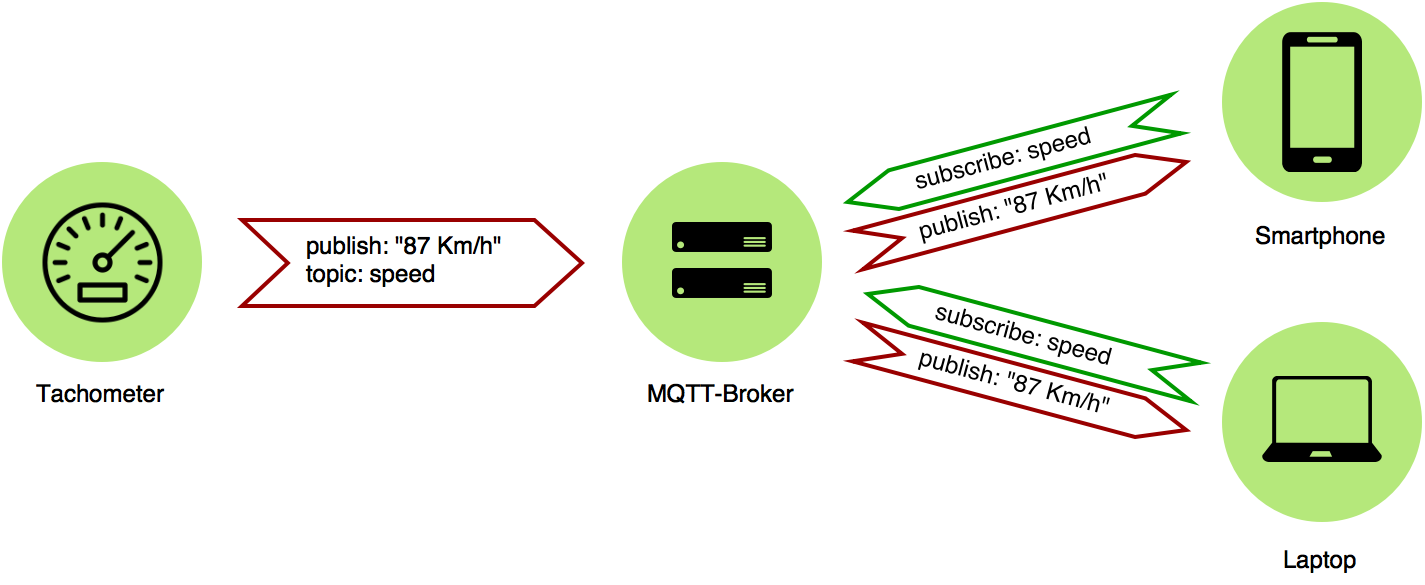
\includegraphics[scale=0.3]{98_Bilder/02_Grundlagen/MQTT}
  \caption[\gls{MQTT} Architektur]{Die Publish/Subscribe Architektur von \gls{MQTT}}
\end{figure}
Der Unterschied zum HTTP Protokoll ist, das ein dienstanforderndes Gerät die Informationen nicht holen muss, sondern direkt geliefert bekommt. Voraussetzung dafür ist eine immer offene TCP Verbindung vom Client zum Server. Falls diese Konnexion unterbrochen werden sollte, kann der \gls{MQTT} Broker Nachrichten zwischenlagern und dann pushen, wenn dieser wieder Verfügbar ist (vgl. \cite{hive:mqtt}).

\section{Node-RED}
Node-RED ist ein Open Source Tool der Firma IBM. um "`Things"', \gls{API}s und Online Services miteinander zu verbinden. Es ist ein browserbasierender Flusseditor. Es basiert auf Node.js und ist eine effiziente Applikation, um Verbindungen im \gls{IoT} zu erstellen. Es bietet auch die Möglichkeit Aktionen auszuführen, Scripts zu definieren und auch andere Online Services zu koppeln (vgl. \cite{nh:nRed}).

\section{Android und Android Wear}
Google's Android ist das marktführende Betriebssystem (vgl. \cite{stat:spos}), welches in aller Munde ist. Es betreibt Smartphones und Tablets unterschiedlicher Hersteller und ist ein Open-Source Produkt. Android Wear ist das OS von Google für Wearables, wie Smartwatches. Es basiert auf Android, ist optimiert für kleine Geräte mit weniger Leistung und kurzer Akkuausdauer.

\section{siot.net}
Die Plattform siot.net ist entstanden, um das Bedürfnis von Nutzern zu stillen, welche Geräte und Dingen ans Internet anbinden wollen, die noch nicht vernetzt sind. Im Interesse der Industriepartner, ist das Ziel diese Plattform zu industrialisieren, um Klein- und Mittlere-Unternehmen (KMU) eine Möglichkeit zu geben ihre Sensoren, Geräte, Maschinen und viele weitere Dinge zu vernetzen. Die Plattform soll ermöglichen, dass auch informatikfremde Personen und Firmen das Internet of Things nutzen können.\\
siot.net bietet ein \gls{IoT}-Center (siehe Abbildung 2.1) mit der \gls{IoT}-Infrastruktur. Konfiguration und Verwaltung werden im \gls{IoT}-Center durchgeführt. Die \gls{IoT}-Infrastruktur beinhaltet einen \gls{MQTT} Broker und das siot-Interface. Das ist die Schnittstellenspezifikation von siot.net. Nicht nach Schema angelieferte Nachrichten kann das \gls{IoT}-Center nicht interpretieren (vgl. \cite{siot:cobo}).\\
\begin{figure}[h]
  \centering
  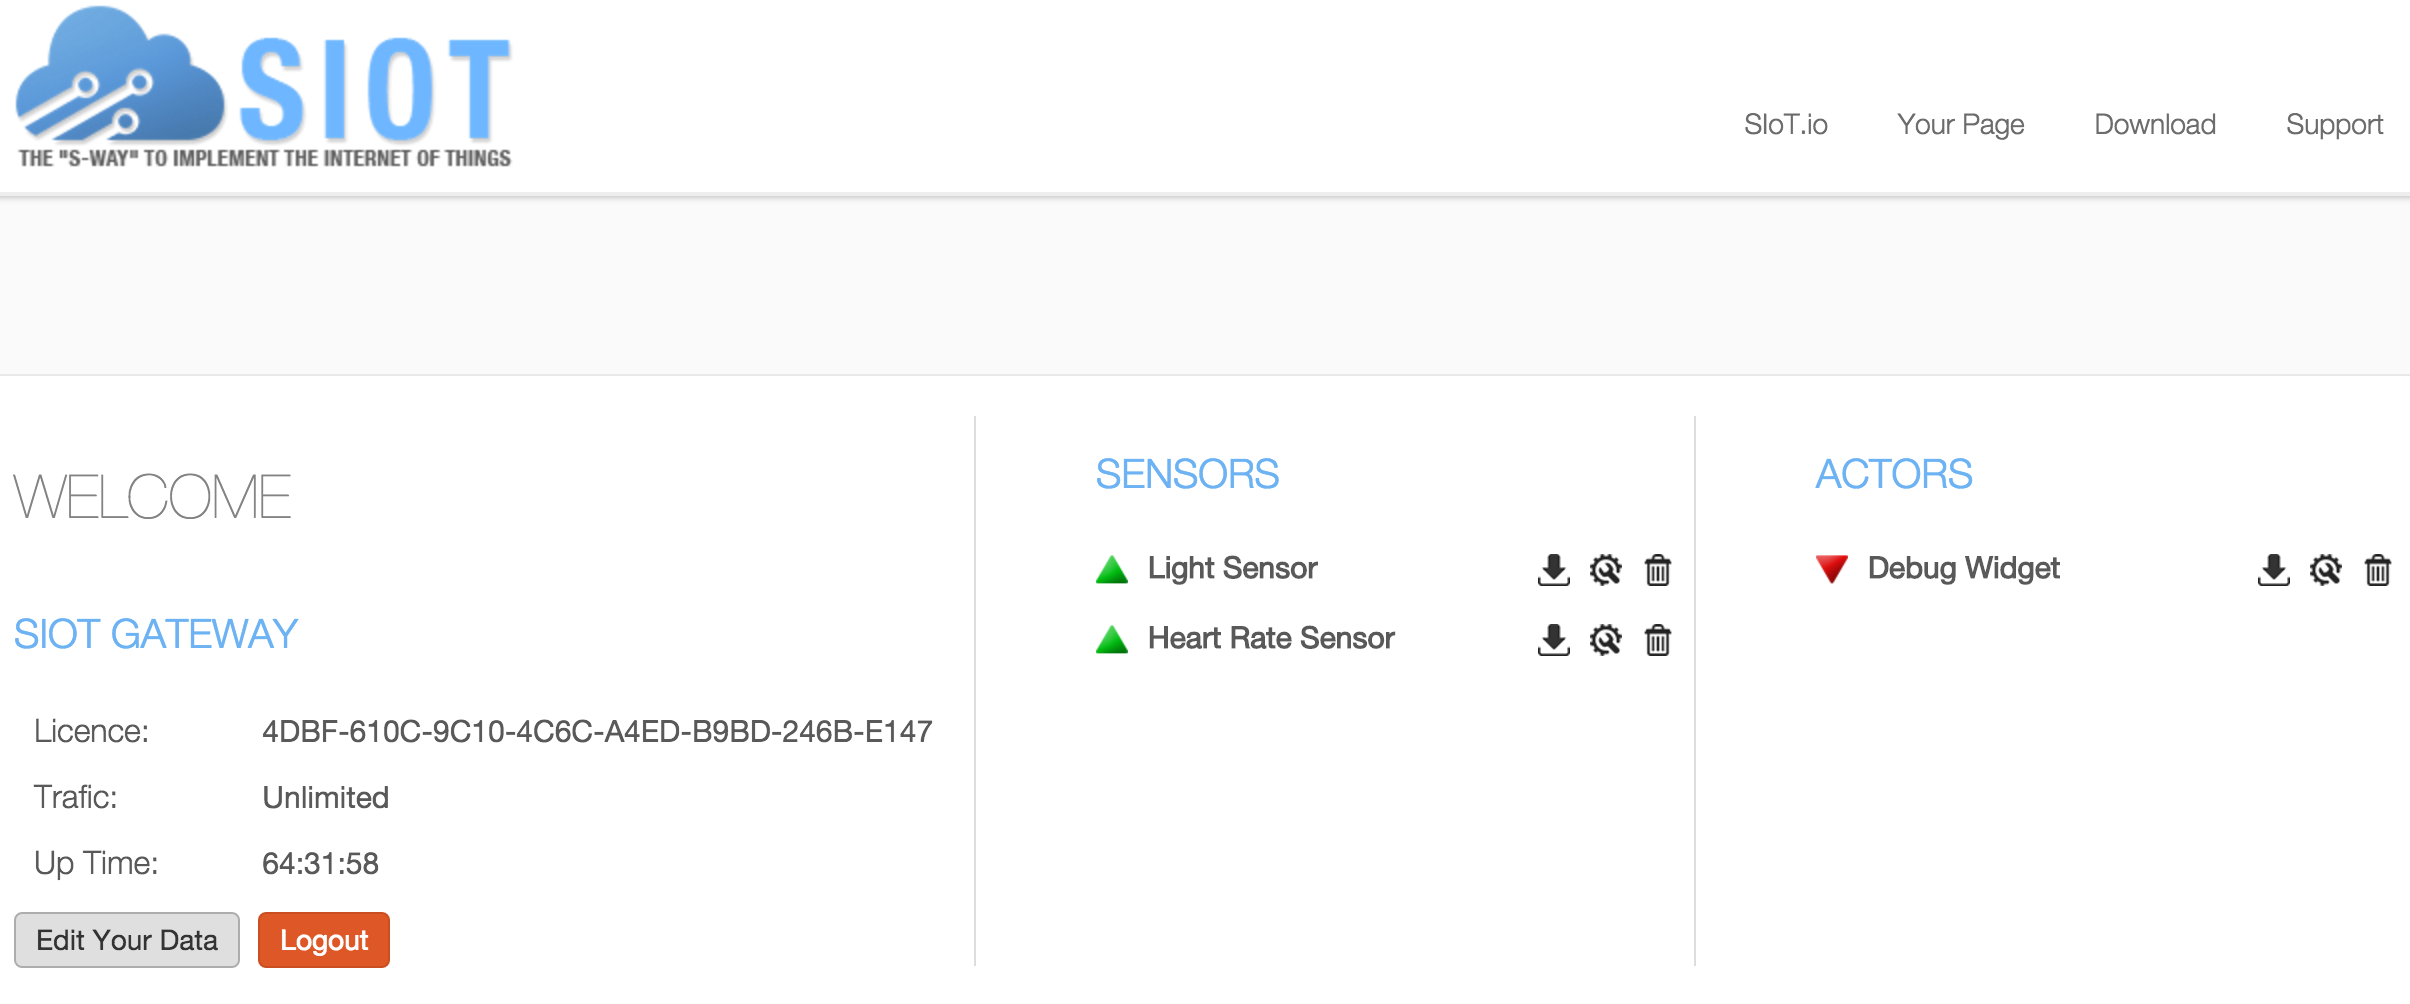
\includegraphics[scale=0.35]{98_Bilder/02_Grundlagen/siotcenter}
  \caption[siot.net IoT-Center]{siot.net \gls{IoT}-Center}
\end{figure}
\section{siot.io}
Für die Verwertung der Daten, welche die siot.net-Plattform sendet und empfängt ist das Projekt siot.io entstanden. siot.io soll die Webschnittstelle zur siot.net-Plattform implementieren. Dabei bietet sie einen Sensorsimulator, eine konfigurierbare Dashboard Applikation mit Widgets, sowie eine Node-RED Instanz für eigene Applikationen.


% Main part - Part III
%---------------------------------------------------------------------------
\onecolumn
\chapter{Marktsegmente}
Im Kapitel Marktsegmente werden die aktuellen Bereiche von Internet of Things, Smartwatches und Smartwatches im Internet of Things aufgezeigt. Es werden Themen aufgelistet und Bereich davon aufgezeigt. Hierfür ist keine strategische Marktsegmentierung durchgeführt worden, dadurch ist es keine abschliessende Auflistung. Für die Evaluation der Marktsegmente wurde der Bericht, The Internet of Things:
Mapping the value beyond the hype von McKinsey Global Institute als Referenz verwendet (vgl. \cite{mk:iot}).

\section{Marktsegmente im Internet of Things}
\begin{tabbing}
xxxxxxxxxxxxxxxxxxxx\=xxxxxxxxxxxxxxxxxxxxxxxx	\kill
Mensch:          \>  Blutdruck, Puls, Bewegungen, Schlafüberwachung, \\\>Körperanalyse {(z.B. Gewicht, Fettanteil, Wasseranteil usw.)} \\
Natur:			     \>  Erdplattenbewegung, Wasserspiegel Überwachung, Temperatur, Wind, Licht, Luft \\
Industrie:  		 \>  Maschinensteuerung, automatisierte Roboter, Lagerüberwachung \\
Heimautomation:	 \>  Nutzung und Überwachung von Haushaltsgeräte, Steuerung, Fernbedienungen \\
Automobil: 		   \>  Telemetrie, Geografische Strecke, Fahrverhalten, Nutzungsverhalten, Verkehrsbericht \\
Städte{/}Verkehr:\>  Touristisches Informationen, Dynamische Strassen, Verkehrsregulierung, Navigation, Lageberichte \\
Detailhandel:		 \>  Produktebezeichnung, Kasse, Geldüberweisung, Geldbörse
\end{tabbing}
Der Auflistung zu entnehmen, kommt das Internet der Dinge in sehr vielen verschiedenen Marktsegmenten zum tragen. Es hat noch grosses unausgeschöpftes Potential den Menschen zu unterstützen um seine Aufgaben zu erleichtern.
\subsection{Mensch}
Der Mensch ist ein wichtiges Marktsegment. Hierbei können Sensoren aller Art den Menschen analysieren. Dieser Punkt wird bei der Marktsegmentanalyse von Smartwatches und Smartwatches im Internet of Things genauer betrachtet.

\subsection{Natur}
Viele verschiedene Anwendungsfälle gibt es auch in der Natur. Es können Sensoren eingesetzt werden, um Temperaturen, Luftdruck, Luftfeuchtigkeit oder Windstärke zu messen. Mit Kombinationen von Sensoren, welche miteinander kommunizieren, können Frühwarnsysteme von Naturkatastrophen erschaffen werden. Dieses Segment hängt sehr nahe mit dem Marktsegment des Menschen zusammen.
%\begin{figure}[H]
%  \centering
%  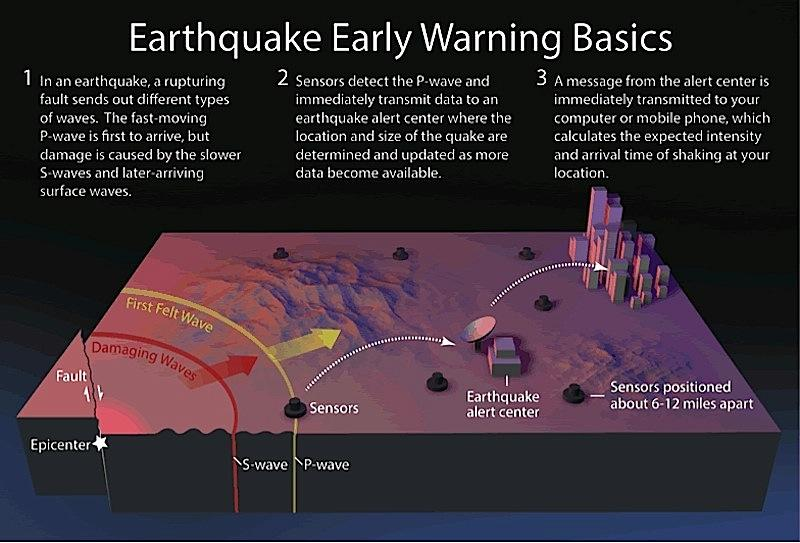
\includegraphics[scale=0.85]{98_Bilder/03_Marktsegmente/erdbeben}
%  \caption[Frühwarnsystem von Erdbeben]{Wie ein Frühwarnsystem von Erdbeben funktioniert}
%  \footnotesize Quelle: \url{http://www.ingenieur.de/var/storage/images/media/ingenieur.de/bilder/funktionsweise-fruehwarnsystems-shakealert/3666615-1-ger-DE/Funktionsweise-des-Fruehwarnsystems-ShakeAlert_image_width_884.jpg}, Stand: 05.11.2015
%\end{figure}
\subsection{Industrie}
Das Internet der Dinge kommt in der Industrie soweit zum tragen, dass man von Industrie 4.0 spricht. Dies soll die vierte industrielle Revolution zum Ausdruck bringen. Die Fertigungstechnologie soll informatisiert werden. Auch die Logistik soll ihre Automatisierung erleben. Erreicht wird dies, weil Maschinen untereinander kommunizieren können. Möglichst alle Sektoren einer Fabrik sollen vernetzt sein. Das Ziel der Industrie 4.0 ist die intelligente Fabrik.
%\begin{figure}[h]
%  \centering
%  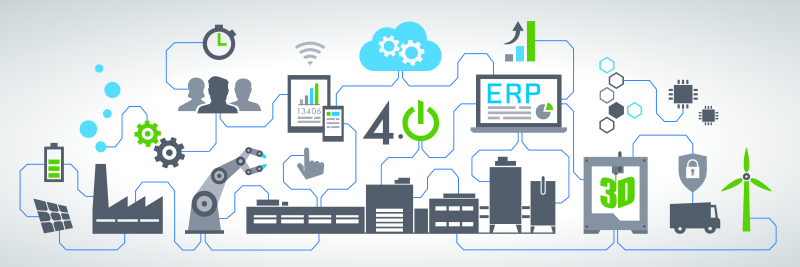
\includegraphics[scale=0.62]{98_Bilder/03_Marktsegmente/industrie4}
%  \caption[Industie 4.0 Symbolbild]{Industie 4.0}
%  \footnotesize Quelle: \url{https://www.scopevisio.com/ratgeber/wp-content/uploads/2015/11/Industrie-4.0.png}, Stand: 05.11.2015
%\end{figure}
%\newpage

\subsection{Heimautomation}
Die Heimautomation ist auch besser bekannt als Smart Home. Smart Home dient als Oberbegriff für technische Verfahren und Systeme in Wohnräumen und -häusern, in deren Mittelpunkt eine Erhöhung von Wohn- und Lebensqualität, Sicherheit und effizienter Energienutzung auf Basis vernetzter und fernsteuerbarer Geräte und Installationen sowie automatisierbarer Abläufe steht.

Unter diesen Begriff fällt sowohl die Vernetzung von Haustechnik und Haushaltsgeräten (z.B. Lampen, Jalousien, Heizung, aber auch Herd, Kühlschrank und Waschmaschine), als auch die Vernetzung von Komponenten der Unterhaltungselektronik (wie etwa die zentrale Speicherung und heimweite Nutzung von Video- und Audio-Inhalten).

Von einem Smart Home spricht man insbesondere, wenn sämtliche im Haus verwendeten Lampen, Taster und Geräte untereinander vernetzt sind, Geräte Daten speichern und eine eigene Logik abbilden können. Geräte sind teilweise auch getagged. Dies bedeutet, dass zu den Geräten im Smart Home Informationen z.B. über Hersteller, Produktnamen und Leistung hinterlegt sind. Dabei besitzt das Smart Home eine eigene Programmierschnittstelle, die (auch) via Internet angesprochen und über erweiterbare Apps gesteuert werden kann.

Eng verwandt mit diesen Verfahren und Systemen sind solche des Smart Metering, bei denen der Schwerpunkt auf dem Messen und einer intelligenten Regulierung des Energieverbrauchs liegt (vgl. \cite{wiki:smho}).
%\begin{figure}[h]
%  \centering
%  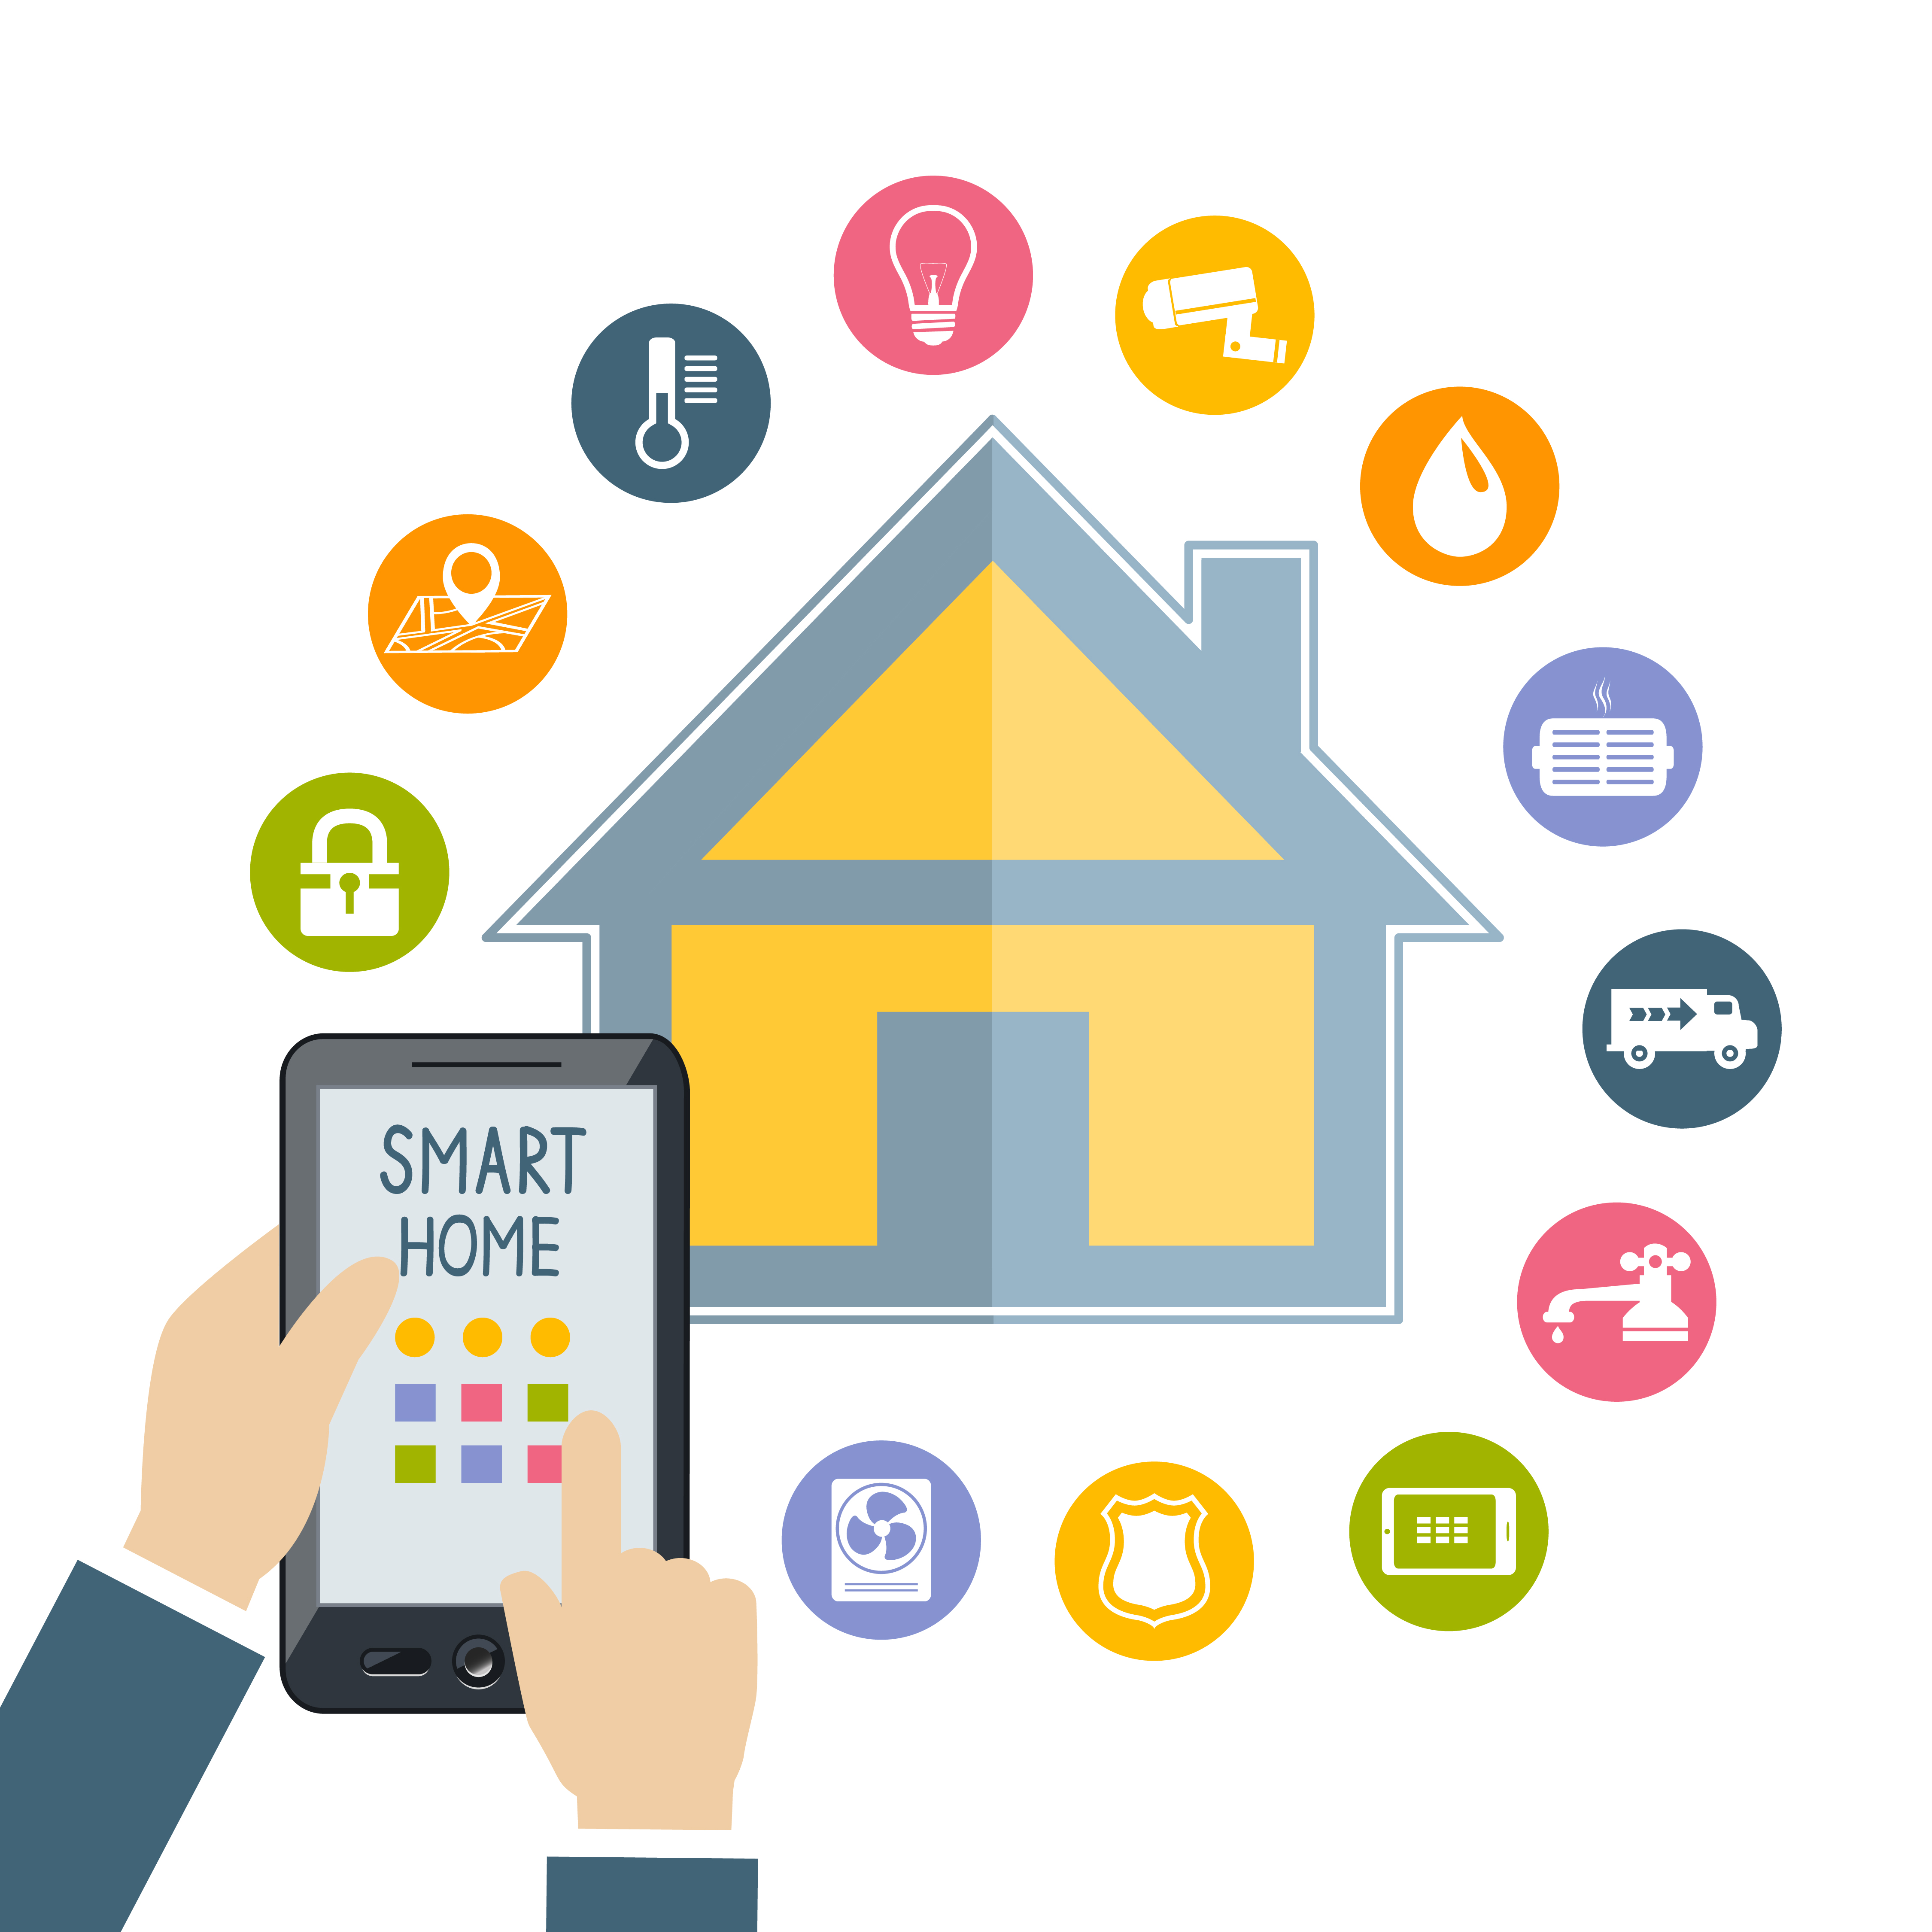
\includegraphics[scale=0.75]{98_Bilder/03_Marktsegmente/smarthome}
%  \caption[Smart Home Symbolbild]{Smart Home}
%  \footnotesize Quelle: \url{http://icon.asid.org/wp-content/uploads/2014/11/40349344_thumbnail.jpg}, Stand: 05.11.2015
%\end{figure}
%\newpage

\subsection{Automobil}
\gls{IoT} kann in vielen Bereichen der Automobilbranche eingesetzt werden. Es können wichtige Daten des Fahrzeugs ausgelesen werden, z.B. die Telemetriedaten. Diese können verwendet werden um das Fahrverhalten vom Lenker festzustellen. Des Weiteren kann, durch Nutzen der Daten, Probleme beim Auto ausgemacht und direkt Fahrer und Mechaniker alarmiert werden.
Interessant, für die Autobauer wie auch Autobesitzer, ist die Ortung der Fahrzeuge. Mit den aufgezeichneten geografischen Punkten kann analysiert werden, wie das Automobil verwendet wird und aktuelle verkehrsnahe Verkehrsberichte können genutzt werden. Die Vollendung der Vernetzung von Fahrzeugen ist das selbstfahrende Auto, welches alle nötigen Informationen empfängt, analysiert und verwendet, um das Ziel optimal zu erreichen.\\
Mercedes-Benz hat ein solches selbstfahrendes Forschungsfahrzeug entwickelt (vgl. \cite{mcbz:f015}). Die Abbildung 3.1 zeigt, wie das Fahrzeug durch die Sensoren einen Fussgänger erkennt und die Laserprojektionstechnik als Aktor verwendet, um dem Überquerenden die Fussgängerstreifen anzuzeigen.
\begin{figure}[h]
%  \centering
%  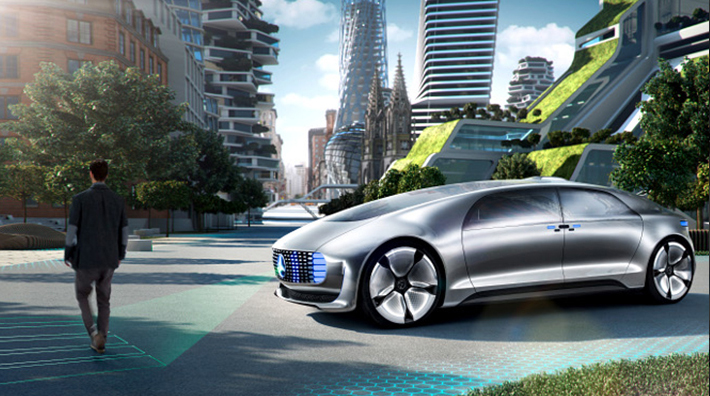
\includegraphics[scale=0.66]{98_Bilder/03_Marktsegmente/mercedesbenzf}
%  \caption[Selbstfahrendes Auto Mercedes-Benz F015 In Motion]{Das selbstfahrende Forschungsfahrzeug von Mercedes-Benz (Modell F015 In Motion)}
%  \footnotesize Quelle: \url{http://www.mercedes-benz.ch/content/media_library/f_015_luxury_in_motion_layer-gallery_1_01__710x396_01-2015.jpg}, Stand: 05.11.2015
  \centering
  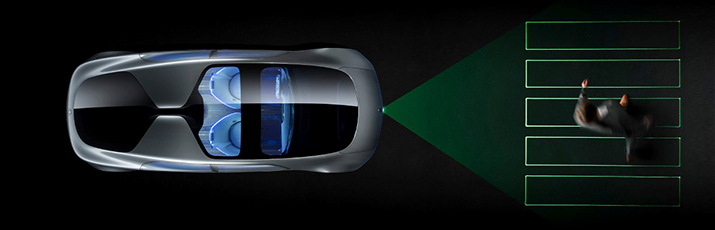
\includegraphics[scale=0.66]{98_Bilder/03_Marktsegmente/mercedesbenzf2}
  \caption[Fussgängererkennung des Mercedes-Benz F 015]{Der Mercedes-Benz F 015 erkennt Fussgänger mit seinen Sensoren}
  \footnotesize Quelle: \url{http://www.mercedes-benz.ch/content/media_library/f_015_luxury_in_motion_gallery_05_715x230_01-2015.jpg}, Stand: 05.11.2015
\end{figure}
\newpage

\subsection{Städte und Verkehr}
In Städten gibt es sehr viele Möglichkeiten. In Verbindung mit dem Verkehr geht dies ins unermessliche. Ein sehr interessantes Thema ist die Touristik. Um ein Beispiel zu nennen: Beacons, welche nötige Information an ein smartes Gerät publizieren, um Daten von der Sehenswürdigkeit abzurufen. Dazu könnte auch gleich Empfehlungen in der Umgebung notifiziert werden. So würde für die meisten Reisenden der Reiseführer wegfallen.

Ein spektakuläres Projekt ist die dynamische Strasse: \textbf{Solar Roadways}. Das sind kleine, feste Platten, welche Photovoltaik-Elementen, Elektronik, verschiedenen Sensoren und \gls{LED}s integrieren (siehe Abbildung 3.2). Die Platten können wie Pflastersteine verlegt und miteinander verbunden werden. Durch die Sonneneinstrahlung sind sie permanent und umweltschonend mit Strom versorgt. Die \gls{LED}s können zentral gesteuert werden, um so die Fahrbahnmarkierungen anzuzeigen und z.B. aus zwei breiten Spuren drei schmale machen, spontane Parkflächen oder Verkehrszeichen. Die Sensoren können feststellen, wenn Tiere oder Menschen darüber laufen und die Fahrer, schon ein paar hundert Meter vorher, über die \gls{LED}s warnen. Und die Platten sind beheizbar. Dies erhöht die Verkehrssicherheit und verringert vermutlich Baustellen. Es wurde von Privatpersonen initiiert und gecrowdfunded. Das Vorhaben ist auf Indiegogo (\url{www.indiegogo.com}) im Juni 2014 deutlich überfinanziert abgeschlossen worden. In Holland hat man im Jahr 2014 begonnen, Radwege auf diese Weise zu bauen (vgl. \cite{hoco:sorw}).
\begin{figure}[h]
  \centering
  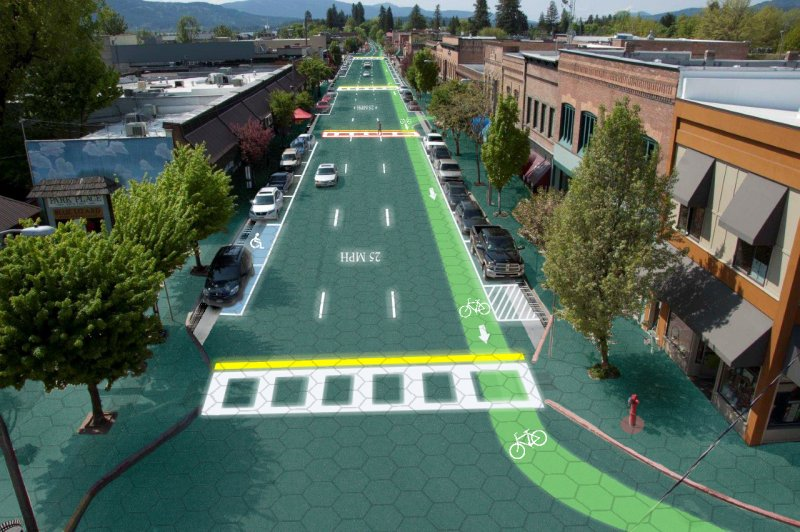
\includegraphics[scale=0.61]{98_Bilder/03_Marktsegmente/solar_roadway_00}
  \caption[Solar Roadway, dynamische Strasse]{Das Solar Roadway verändert die Strasse für die aktuelle Verkehrsituation}
  \footnotesize Quelle: \url{http://www.solarroadways.com/images/intro/Downtown%20Sandpoint%202%20-%20small.jpg}, Stand: 05.11.2015
\end{figure}
%\newpage
%\begin{figure}[H]
%  \centering
%  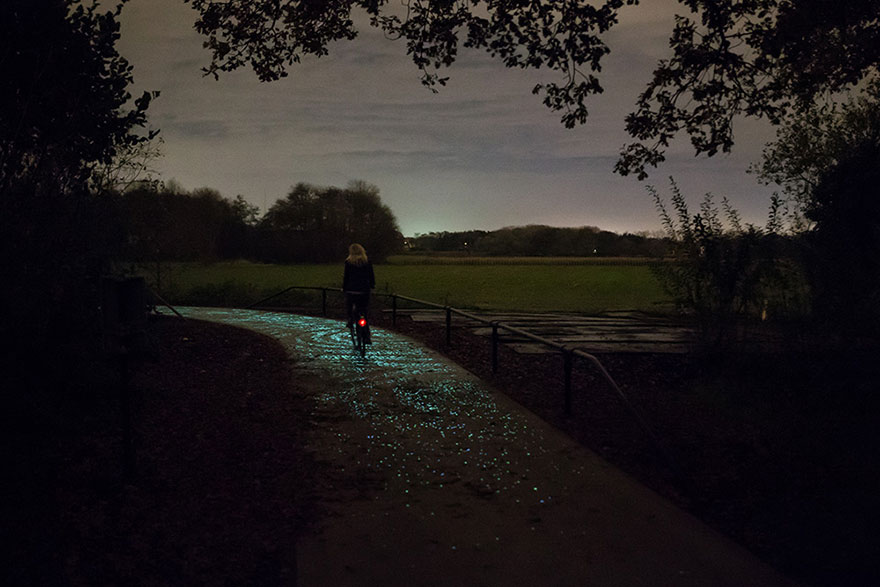
\includegraphics[scale=0.5]{98_Bilder/03_Marktsegmente/solar_roadway_02}
%  \caption[Solar Roadway in der Dämmerung]{Solar Roadway: In der Dämmerung wird der Weg an den nötigen Stellen beleuchtet}
%  \footnotesize Quelle: \url{http://static.boredpanda.com/blog/wp-content/uploads/2014/11/van-gogh-starry-night-glowing-bike-path-daan-roosengaarde-2.jpg}, Stand: 05.11.2015
%  \centering
%  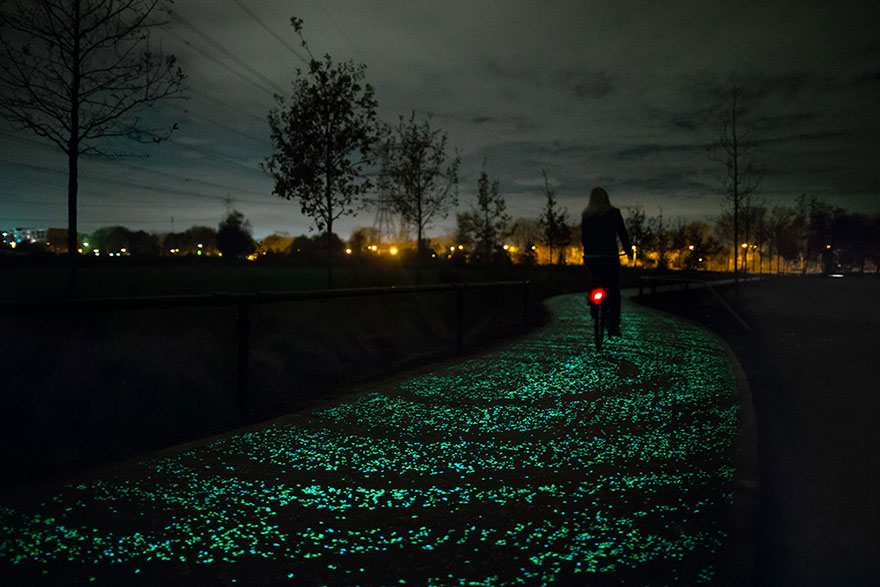
\includegraphics[scale=0.5]{98_Bilder/03_Marktsegmente/solar_roadway_01}
%  \caption[Solar Roadway bei Nacht]{Solar Roadway: Bei Nacht ist der Veloweg komplett beleuchtet}
%  \footnotesize Quelle: \url{http://static.boredpanda.com/blog/wp-content/uploads/2014/11/van-gogh-starry-night-glowing-bike-path-daan-roosengaarde-1.jpg}, Stand: 05.11.2015
%\end{figure}
\newpage

\subsection{Detailhandel}
Im Verkauf hat die Revolution schon teilweise begonnen. Die grossen Unternehmen in der Schweiz beginnen alle ihre Filialen mit \gls{WLAN} auszustatten. Momentan bieten diese den \gls{WiFi} Zugang zur freien Verfügung den Kunden an. Somit steht der Kommunikationskanal für das \gls{IoT} im Laden bereit und die Kunden sind zur gegebenen Zeit bereits verbunden damit.
Weiter werden heutzutage Selbstbezahlkassen eingesetzt. Momentan werden zwei Modelle verfolgt. Eine Einkaufsart ist: Der Kunde wählt seine Produkte und scannt diese selber ein, bezahlt mit Karte oder Bar und verlässt das Geschäft. Bei der \gls{IoT} näheren Methode, registriert sich der Konsument beim Eingang an einem Terminal und rüstet sich mit einem mobilen Strichcodeleser der Filiale aus oder nimmt sein Smartphone als Scanner. Die Person liest alle Produkte mit dem Scanner ein und bezahlt, beim verlassen des Ladens, am Bezahlterminal. Beim abmelden des Scanners wird der Kunde ermittelt und das Total eingefordert.\\
Ein weiterer Schritt ist hier, alle Produkte mit einer \gls{RFID} zu taggen. Somit könnte der Kunde nur seine Kreditkarte registrieren, die Ware in den Einkaufskorb legen und die Filiale verlassen. Beim verlassen wird durch die Information auf dem \gls{RFID} Tag gemerkt, welche Ware mitgenommen wurde und die Kreditkarte wird automatisch belastet.
%\begin{figure}[H]
%  \centering
%  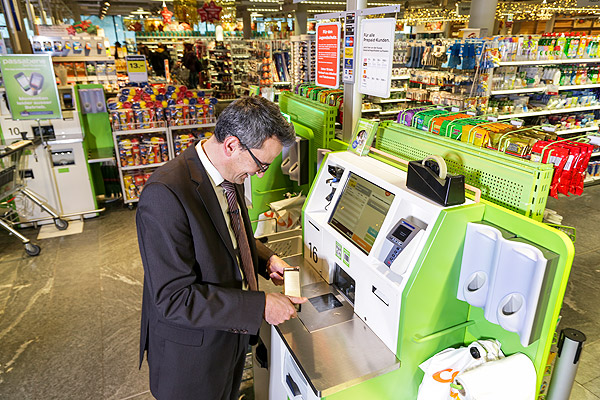
\includegraphics[scale=0.81]{98_Bilder/03_Marktsegmente/self_checkout}
%  \caption[Self Checkout Kasse]{Eine Selbstbezahlkasse für mit mobilen Scanner oder zum selber einlesen}
%  \footnotesize Quelle: \url{https://www.cooperation.ch/site/presse/get/12946772/Sutter-Selfscan_198B0923.jpg}, Stand: 05.11.2015
%\end{figure}

\section{Marktsegmente für Smartwatches}
\begin{tabbing}
xxxxxxxxxxxxxxxxxxxx\=xxxxxxxxxxxxxxxxxxxxxxxx	\kill
Mensch:		          \> Blutdruck, Puls, Bewegungen, Schlafüberwachung, Lebensüberwachung, \\\>Sportbeobachtungen, Sporttracking \\
Zeit:			          \> Individuelle Zeitansichten, Zeitfunktionen \\
Benachrichtigung:	  \> Informationen am Handgelenk, Kommunizieren
\end{tabbing}
Momentan werden Smartwatches hauptsächlich zu Notifikationszwecken und Fitnesstracking des Menschen genutzt. Noch wird das Potenzial nicht ausgenutzt Smartwatches in vielen anderen Segmenten einzusetzen. Um dies zu ermöglichen müssen die Bedürfnisse zuerst erkannt oder geschaffen werden.

\subsection{Mensch}
Heute werden Smartwatches verwendet, um den Menschen bei Aktivitäten überwachen zu können. Diese Wearables verfügen viele eingebaute Sensoren, die die Bewegungen des Trägers analysieren und dem interessierten die Daten zur Verfügung stellen. Zu den Sensoren gehören z.B. ein Bewegungssensor, Schrittzähler, Herzfrequenzmesser und viele mehr. Viele Hersteller von Smartwatches rüsten Ihre Produkte mit Sensoren und mit Auswertungsapplikationen (z.B. Google Fit, Apple Health oder Motorola Moto Body) aus. Mit diesen Apps kann der User seine Daten während dem Training auf der Uhr verfolgen oder später auf dem Smartphone auswerten. Dies macht zusätzliche Sport-/Pulsuhren überflüssig.

\subsection{Zeit}
Die Hauptaufgabe einer Uhr ist es, die Uhrzeit genau anzuzeigen. Die Smartwatches haben nicht nur die Möglichkeit die aktuelle Uhrzeit anzuzeigen, sondern auch als Weltuhr, Stoppuhr und Countdown-Rechner zu fungieren. Dabei hat der Träger der Computeruhr die Wahl, wie das Ziffernblatt aussehen soll. Wie individuell sie gestaltet werden wird vom Benutzer oder Entwickler bestimmt. Für Individualisten ist sie sehr geeignet.
%\begin{figure}[H]
%  \centering
%  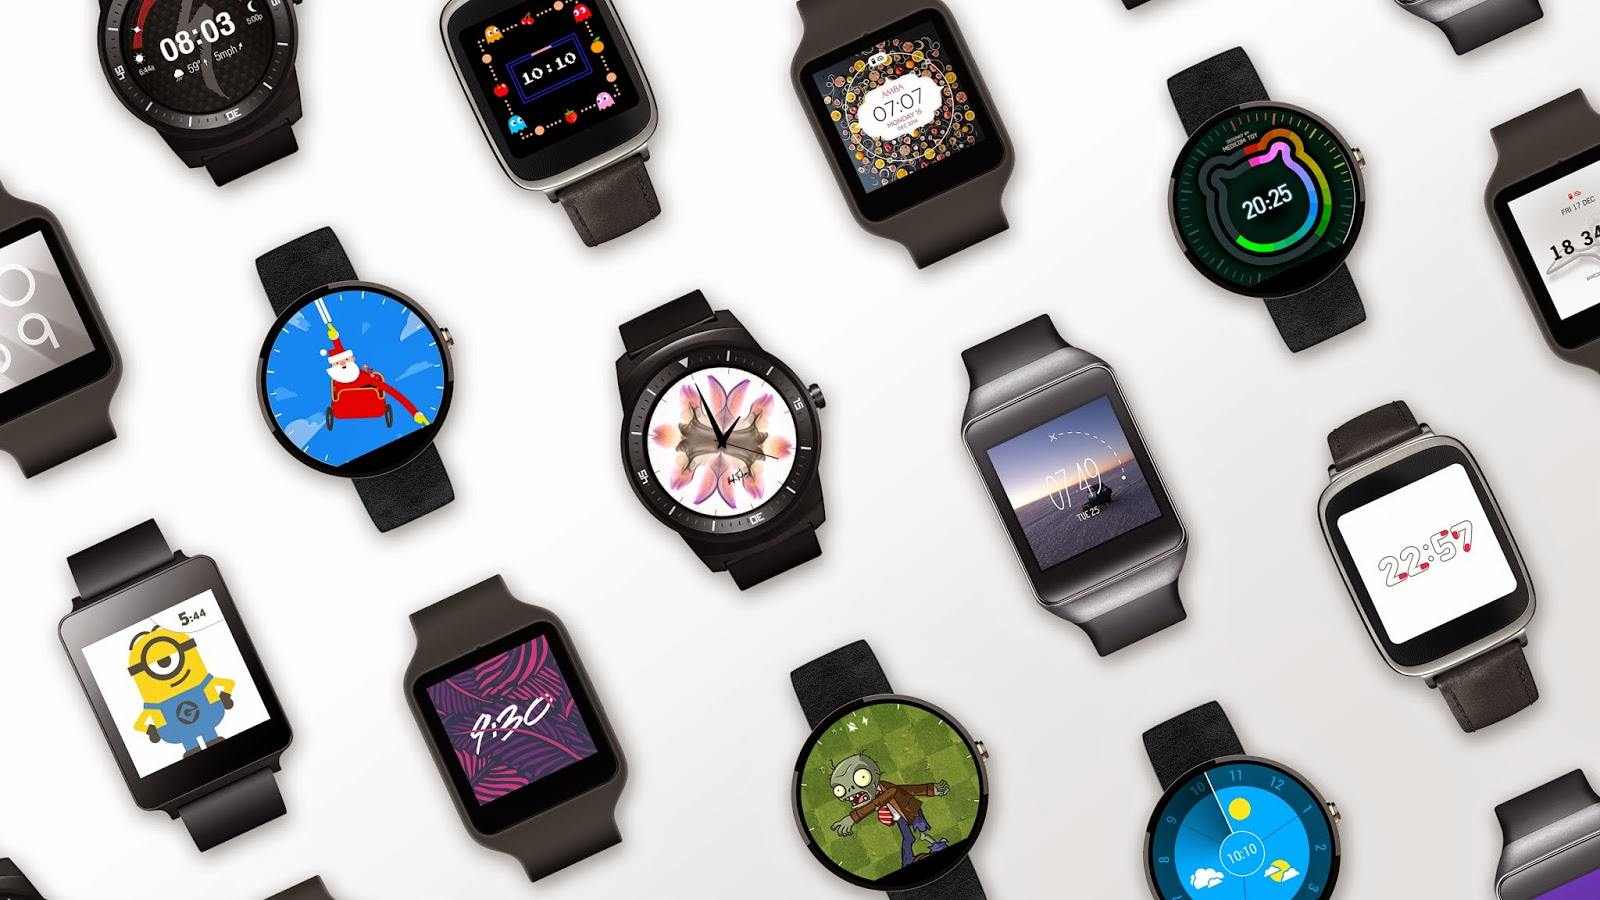
\includegraphics[scale=0.25]{98_Bilder/03_Marktsegmente/smartwatchfaces}
%  \caption[Smartwatch Ziffernblätter]{Das Ziffernblatt der meisten Smartwatches kann individuell gestaltet werden}
%  \footnotesize Quelle: \url{http://i1-news.softpedia-static.com/images/news2/Google-Launches-Watch-Face-API-You-Can-Customize-Your-Smartwatch-467130-2.jpg}, Stand: 12.11.2015
%\end{figure}

\subsection{Benachrichtigung}
Eine Smartwatch wird neben der Uhrzeitfunktion auch als Notifikationsbildschirm verwendet. Alle relevanten Benachrichtigungen an ein Smartphone können auch von der Smartwatch angezeigt werden. Dabei dient die Uhr meist als verlängerter Arm des Mobilgerätes. Es können Nachrichten empfangen, Telefonate geführt, Erinnerungen ausgelöst, der Wecker gestellt werden oder anzeigen was auf dem Smartphone ausgeführt wird, z.B aktuell abgespieltes Musikstück.
%\begin{figure}[H]
%  \centering
%  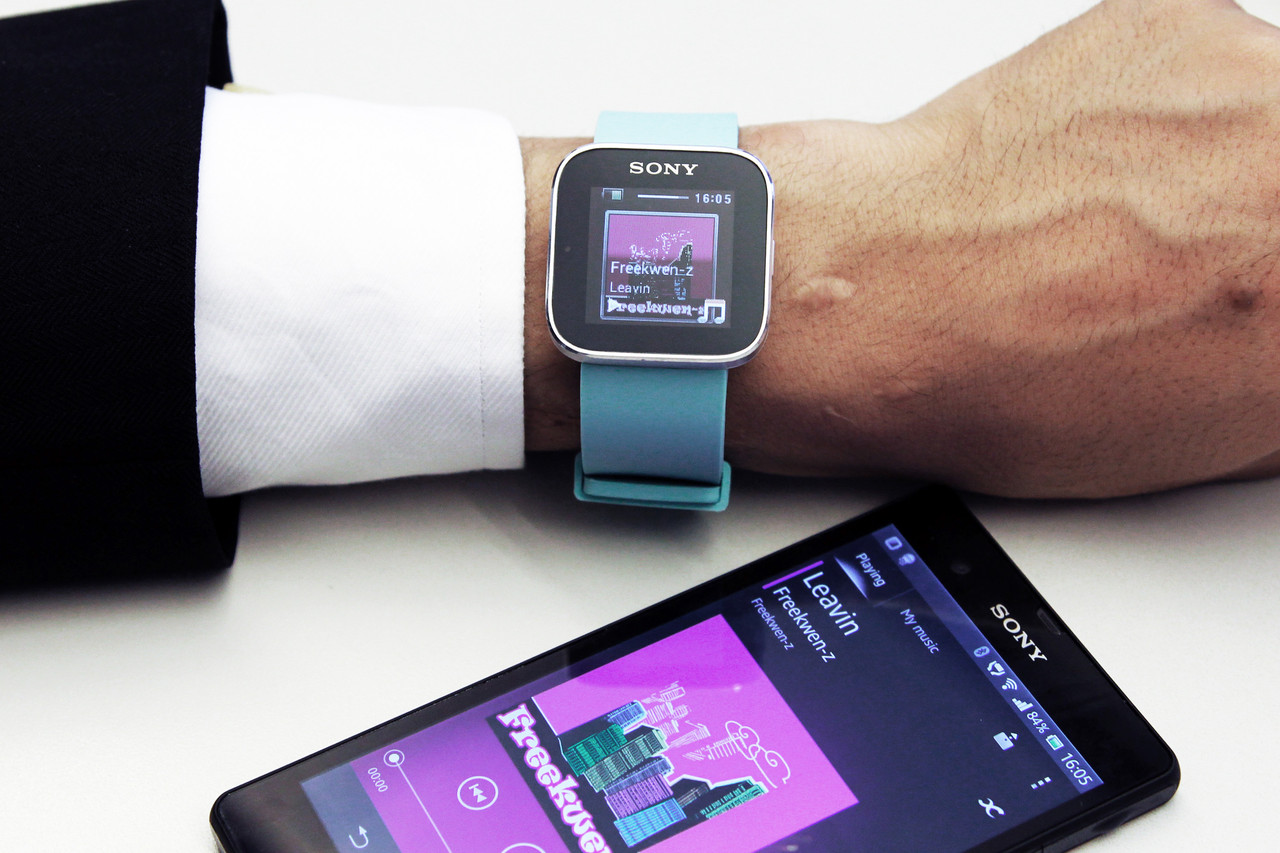
\includegraphics[scale=0.3]{98_Bilder/03_Marktsegmente/notifications}
%  \caption[Smartwatch Anzeige von Smartphone]{Die Smartwatch zeigt an, welches Musikstück auf dem Smartphone abgespielt wird}
%  \footnotesize Quelle: \url{http://smartwatchpro.it/wp-content/uploads/2015/08/OB-YT760_smartd_M_20130904020012.jpg}, Stand: 12.11.2015
%\end{figure}
%\newpage

\section{Marktsegmente für Smartwatches im Internet of Things}
\begin{tabbing}
xxxxxxxxxxxxxxxxxxxx\=xxxxxxxxxxxxxxxxxxxxxxxx	\kill
Mensch:		        \> Blutdruck, Puls, Bewegungen, Schlafüberwachung, Gesundheitsbenachrichtigung \\
Benachrichtigung:	\> Alarme, Informationen \\
Heimautomation:	  \> Fernbedienung, Statusanzeigen, Alarming \\
Detailhandel:		  \> Geldbörse, Produktebezeichnung, Einkaufsliste \\
Ortsbezogen:		  \> Navigation, Ortsspezifische Informationen, Ortung, Personen in der Nähe \\
\end{tabbing}

\subsection{Mensch}
Um die Gesundheit eines Menschen zu überwachen, eignet sich eine Smartwatch sehr gut. Sie ist immer am Handgelenk und kann bei Unregelmässigkeiten Alarm schlagen. Durch die Vernetzung werden die Daten auch an anderen Geräten zur Verfügung gestellt. Eine wichtige Benachrichtigung kann von einer anderen Smartwatch oder einem Smartphone verwendet werden. Ein sich vorstellbares Szenario: Ein Paar, beide tragen eine smarte Uhr, bei einer potenziellen Gefahr, z.B. schwacher/kein Puls, Sturz, ungewöhnliche Bewegungsabläufe, wird der Andere alarmiert.

\subsection{Benachrichtigung}
Um Informationen darzustellen, eignet sich eine Smartwatch nur beschränkt so gut, wie ein Smartphone oder andere grössere Anzeigeapparate. Sie ist jedoch prädestiniert einzelne kleine Datenmengen anzuzeigen. Die im Internet der Dinge übermittelten und verwerteten Daten, können für den Menschen, auf einem praktisch sichtbaren Display am Handgelenk, angezeigt werden. Dies gewährt einen schnellen Zugriff zu den Benachrichtigungen.
%\begin{figure}[H]
%  \centering
%  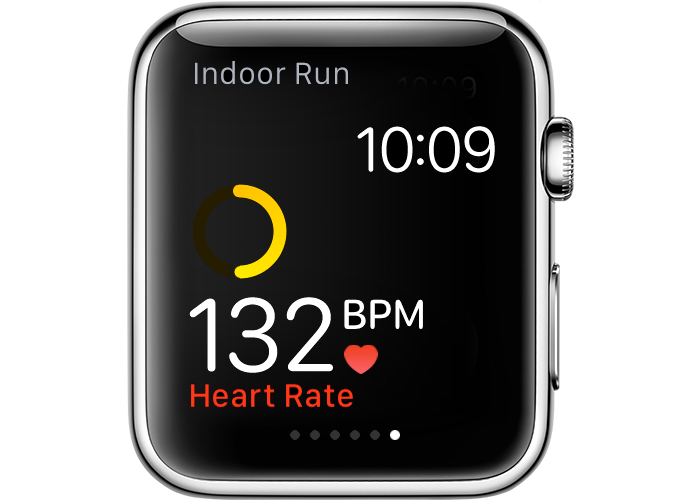
\includegraphics[scale=1]{98_Bilder/03_Marktsegmente/infodisplay}
%  \caption[Smartwatch Anzeige von Tätigkeiten]{Die Smartwatch zeigt an, welche Herzfrequenz der Träger hat und wie lange er eine Tätigkeit ausführt}
%  \footnotesize Quelle: \url{https://support.apple.com/images/en_US/applewatch/watch-indoor-workout-heartrate.png}, Stand: 20.11.2015
%\end{figure}

\subsection{Heimautomation}
Im Smart Home Bereich kann die Kombination Smartwatch und Internet of Things ihre stärken ausspielen. Durch den Zusammenschluss aller Haushaltgeräte, wie Fernseher, Lampen oder Herdplatte, sind alle Daten zentral erreichbar und verwaltbar. Nun bestehen viele Möglichkeiten die Computeruhr ins System einzubinden. Einige geeignete Anwendungsfälle sind: Das Licht ein- und auszuschalten, Alarmierung von nicht ausgeschalteten Haushaltsgeräten oder das Fernbedienen von Geräten. All dies soll unabhängig vom Ort des Uhrträgers möglich sein.

\subsection{Detailhandel}
Im Detailhandel sind besonders Finanztechnologie Applikationen schon stark vertreten, wie Apple Pay, Google Wallet oder auch die schweizerische Lösung TWINT. Diese Anwendungen erlauben Geldüberweisungen mit Smartphones oder Smartwatches mittels drahtloser Verbindung über ein Terminal, welches die Bezahlung anfordert.\\
Des weiteren könnten Smartwatches in Selbstbedienungsgeschäften als erweiterter Informationsschild von Produkten dienen. Durch die Anbindung ans Internet hat man die Möglichkeit, jedes weitere Detail, welches nicht auf der Ware beschrieben ist, auf dem Bildschirm am Arm anzuschauen. Ein sehr grosser Vorteil ist, dass verschiedene Medien genutzt werden können, z.B. detailliert Nährwertangaben, Anleitungsfilme aller Art, Explosionszeichnungen von Modellen und viele weitere.

\subsection{Ortsbezogen}
Applikationen für die Ortung oder zur Anzeige standortabhängiger Daten werden bei vielen Anwendungen benutzt. Dies auf die Smartwatch zu erweitern ist ein logischer Schritt. Ein ortsrelevantes Thema kann direkt am Handgelenk angeschaut werden ohne das Smartphone heranzuziehen.
%\begin{figure}[H]
%  \centering
%  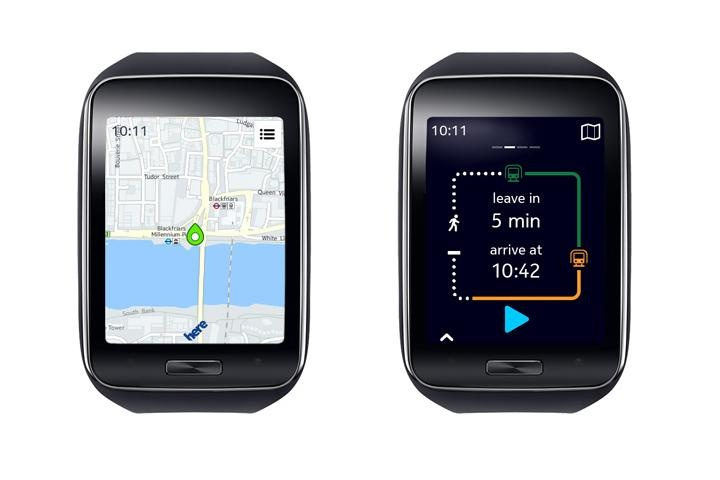
\includegraphics[scale=.5]{98_Bilder/03_Marktsegmente/watchmaps}
%  \caption[Smartwatch und ortsrelevante Informationen]{Landkarten anzeigen und ortsrelevante Informationen sind auf Smartwatches möglich}
%  \footnotesize Quelle: \url{http://icdn9.digitaltrends.com/image/here-maps-samsung-gear-s-720x480.jpg?ver=1}, Stand: 20.11.2015
%\end{figure}


% Main part - Part IV
%---------------------------------------------------------------------------
\onecolumn
\chapter{Bedürfnisanalyse}

Im Kapitel der Bedürfnisanalyse werden Anwendungsfälle ermittelt welche mit Smartwatches abgedeckt werden können. Zusätzlich wird eine Bedarfsanalyse durchgeführt für Applikationen welche in Verbindung zur siot.net Plattform stehen.
\section{Smartwatch Applikationen}
\subsection{Gesundheit}
Im Gesundheitssektor gibt es einige Anwendungsfälle welche mit einer smarten Uhr abgedeckt werden können.

Eine Smartwatch bietet die Möglichkeit sich zu überwachen. Da die Computeruhr mit vielen Sensoren, wie z.B. Bewegungsensor oder Herzfrequenzmesser, ausgerüstet ist, hat sie die Möglichkeit den Träger sehr genau zu analysieren.

Bei einem Sturz des Benutzers kann ein Alarm ausgelöst werden. Dieser würde in erster Instanz eine positive Gesundheitsbericht des Anwenders verlangen. Diese Bestätigung sollte in einem definierten Zeitrahmen statt finden. Falls dies nicht ausgeführt wird und die Uhr keine Bewegung registriert, kann ein Alarm an eine Vertrauensperson oder gar ein Notruf ausgelöst werden. Dieser Notruf kann wichtigen Daten angereichert werden, wie z.B. Pulsdaten und die GPS Koordinaten. Statt des Sturzes kann hier der Auslöser des Alarmes auch ein zu tiefer oder gar kein Puls sein.

Ein weiterer nützlicher Use-Case ist, Alarme von Patienten im Spital. Hier kann das Pflegepersonal mit Smartwatches, Patientenalarme erhalten. Die Alarme sollten möglichst nur empfangen werden, wenn der Patient in der nähe des Patienten sich befindet. Wenn mehrere Pfleger/innen benachrichtigt werden, kann eine Pflegeperson den Alarm bestätigen und die Verantwortung für den Patient übernehmen, so können Doppelspurigkeiten vermieden werden.

\subsection{Smart Home}
Für die Fernbedienung von Geräten im Haus oder Wohnung eignet sich die Smartwatch gut. Mit eingebauten Touchscreen und Vibrationsmotor, haben die kleinen Handgelenkrechner die Möglichkeit Informationen visuell wie taktil an die Person zu bringen.

Geräte im Haushalt können überwacht werden. Dies hilft Gefahren abzuwenden. Wenn eine Herdplatt noch läuft kann ein Alarm ausgelöst werden und es kann gleich mit der Uhr reagiert werden und die Platte ausschalten.

Für jeden einen Mehrwert gibt die Funktion Licht vom Handgelenk zu bedienen. Es ist bequem das Zimmer zu beleuchten ohne zum Lichtschalter gehen zu müssen. Dimmen mit dem Touchscreen und terminierte Lichtsteuerung. Auch eine automatische Beleuchtung durch erkennen der Helligekeit im Raum ist eine Funktion mit hohem Potenzial.

Ein weiterer Anwendungsfall ist die Waschmaschine. Die Restzeit des Waschgangs kann auf den Bildschirm angezeigt werden und wenn er beendet ist, wird der Träger mit einem Vibrationsimpuls notifiziert.

Desweiteren ist das Fernbedienen von allen Multimediageräten vom Handgelenk sehr praktisch. Es genügt eine Uhr und braucht nicht mehr viele verschiedene proprietäre Steuerungen. Dies wird heute bereits mit Smartphone Apps praktiziert. Mit Sprachsteuerung können Personen mit eingeschränkter Sehkraft die Uhr verwenden.

\subsection{Sport}
Heute werden Smartwatches hauptsächlich als Fitnesstracker verwendet\footnote{vgl. Studienband Smartwatch Umfrage eResult, Ausgabe: Juni 2015}. Das Praktische an den Uhren unter den Wearables ist, dass diese nicht nur für zum Sport treiben gekauft werden muss. Hier erhält der Endkunde ein Gerät für den Alltag und die Freizeit.

Im Sportbereich kann mit den vorhandenen Sensoren viele verschiedene Werte ermittelt und analysiert werden. Mit den nötigen Voreinstellungen, wie Körpermasse, Schrittlänge, Alter und Geschlecht, ist es möglich Bewegungsdaten genau aufzuzeichnen. Mit den Daten können für den Anwender interessante Informationen berechnet werden. Für Hobbysportler meist relevante Berechnungen sind Zeit, Schritte, Geschwindigkeit und Kalorienverbrauch. Für erfahrene Sportler verbessern ihre Fähigkeiten durch betrachten von Auswertungen der Körperbelastungen, z.B. Beschleunigung, Stärke, Drehmoment und weitere.

\subsection{Ortsbezogen}
Applikationen welche umgebungsorientiert arbeiten, sind geeignete Kandidaten für Smartwatches. Durch die permanente Anzeige am Handgelenk, können schnell ändernde Daten dauerhaft im Auge behalten werden.

Ein Anwendungsfall ist, das Smartphone zu überwachen. Die Uhr kann den Träger informieren, wenn das Sichtbarkeitsumfeld vom Mobiltelefon und des tragbaren Rechners sich nicht mehr überschneiden, was bedeuten würde die Geräte entkoppeln sich voneinander.

Die gleiche Methode bietet sich an, Personen mit Smartwatches in der Nähe zu scannen. Diese Funktion kann bei Partnervermittlungsapplikationen effektiv eingesetzt werden. Durch den vorhandenen Touchscreen können potenzielle Datingpartner angezeigt und kontaktiert werden. In der schnelllebigen Welt sind sich schnell erschliessende Kontakte sehr willkommen.

Ein weiterer Punkt ist Geofencing. Mit Geofencing werden automatische Aktionen eingeleitet. Diese geschehen sobald bestimmte geografische Grenzen überschritten werden. Über eine Ortung des Gerätes kann ermittelt werden ob dieses sich in einer Geofencing Zone befindet. Mit Smartwatches kann dies effektiver genutzt werden, da durch den immer sichtbaren Bildschirm, die ortsrelevanten Daten ohne Zeitverlust angezeigt.\\
Eine Geofencing Anwendung wäre Sehenswürdigkeiten präsentieren. Eine App welche für jede Sehenswürdigkeit eine Geofencing Zone errichtet oder kennt und jeweils die Auskunft des Objektes darstellt.

Die Indoornavigation ist ein Bedürfnis welches mit Smartwatche nicht gelöst jedoch erweitern kann. In Zusammenarbeit mit Beacons/Eddystones und/oder Access Points können die Standorte von Smartwatchträger, im inneren von Räumen, ermittelt werden. Beacons und Eddystones sind Sender/Empfänger welche auf Bluetooth Low Energy (BLE, Bluetooth 4.0 oder  Bluetooth Smart).\\
Grossfirmen können eine grossen Nutzen aus dieser Technologiekombination schöpfen. Die Mitarbeiter ihren Standort preisgeben, damit diese gefunden werden können ohne zu suchen. Es können Geofencing Zonen definiert werden um die Zeiterfassung zu automatisieren. Beim eintretten, des geografisch definierten Bereichs, welcher zu Arbeitszone gehört, wird Arbeitszeit erfasst. Verlässt der Mitarbeiter diesen Teil des Gebäudes, wird die Arbeitszeiterfassung gestoppt.\\
Zusätzlich kann das Problem mit den Shared-Desk Arbeitsplätzen kann gelöst werden. Bei diesem Arbeitsplatzmodell richtet sich der Mitarbeiter jeden Tag an dem Ort ein wo es einen freien Platz hat. Da dieser nicht im vorherein weiss wo der nächste freie Platz ist, führt dies zu Verlusten, wenn Zeit benötigt wird um einen Arbeitsplatz zu suchen. Mit der Smartwatch ausgetattet, ist der Angestellte in der Lage, vorgängig einen freien Arbeitsplatz zu reservieren und sich anzumelden, beim erreichen des Schreibtisches.
\newpage

\subsection{Authentifikation}
Im Authentifikationssektor gibt es einige Bedürfnisse welche mit Smartwatches gedeckt werden können

Türen entrigeln mit der Smartwatch ist ein geeigneter Anwendungsfall. Heute benutzen die meisten Automobilhersteller ein Keyless System für ihre Fahrzeuge. Mit diesen Systemen hat der Fahrer nur ein Sender/Empfänger, mit einem einzigartigem Zertifikat, welches sich mit dem Fahrzeuges korreliert. Türen werden geöffnet und Motoren werden gestartet, diese Funktion könnte auch die Smartwatch übernehmen. Damit hätte der Fahrzeugbesitzer ein Utensil weniger zu mitzutragen.

Die intelligente Uhr hat das Potenzial Personalausweise zu ersetzen. Wie bereits im Abschnitt Ortsbezogen erwähnt kann es zur Zeiterfassung genutzt werden. Das heisst Mitarbeiter muss nicht mehr an die Zeiterfassungsleser.

\subsection{Finanztechnologie - FinTech}
Die Möglichkeit zu haben mit der Uhr Zahlunge zu authorisieren ist ein Bedürfnis, welches erschaffen werden kann. Denn es scheint praktisch einzukaufen gehen ohne das Portmonee dabei zu haben. Es sind Lösungen vorhanden, welche mit Smartphones funktionieren {(Abbildung 4.1 Apple Pay/Google Wallet/TWINT)}. Mit der Lancierung der Apple Watch, erreichte die erste Smartwatch mit einer Zahlfunktion, sie unterstützt Apple Pay, den Markt.

\section{Smartwatch Applikationen für siot.net}
Die siot.net Plattform bietet sich bestens als Kommunikationsschnittstelle an für die Applikationen, welche im vorherigen Abschnitt ermittelt wurden. Die meisten Bedürfnisse verlangen irgendeine Art von Kommunikation. Ob es nur übermitteln der Sensordaten ist oder die Abfrage eines Sicherheitstokens ist, die siot.net Plattform erlaubt sämtliche Informationen über eine Schnittstelle auszutauschen. Damit es einfacher wird sollten möglichst viele oder besser alle Geräte, welche miteinander kommunizieren sollen, an die siot.net Plattform angebunden werden.
\begin{figure}[h]
  \centering
  \includegraphics[scale=0.2]{98_Bilder/04_Anwendungen/APay_GWallet_PFTwint.png}
  \caption[Mobile Zahlungslösungen: Apple Pay, Google Wallet und TWINT powered by PostFinance]{Bekannte Zahlungslösunge für Smartphone: Apple Pay, Google Wallet und TWINT powered by PostFinance}
  \footnotesize \url{http://www.apple.com/apple-pay/} \url{https://wallet.google.com/} \url{http://www.twint.ch/ueber_uns/medien/}, 04.12.2015
\end{figure}

\subsection{siot.net Gateway Library}
Um Verknüpfungen individueller Applikationen von Smartwatches oder auch Smartphones mit der Plattform zu ermöglichen, sollte es eine generische Biblithek geben. Diese sollte eine einfache Schnittstelle implementieren, welche Applikation an die siot.net Plattform anbindet. Eine automatische Erkennung aller Sensoren vereinfacht die Entwicklung von Apps welche zum siot.net IoT-Center kommunizieren wollen.

\subsection{siot.net Sensorcenter}
Jedes Android Gerät kann mit den eingebauten Sensoren hervoragend als Sensorstation dienen. Um die Vielzahl von Sensor in Eigenregie zu im siot.net zu manifestieren und Sensordaten preiszugeben, sollte es ein App geben mit einer möglichst eifachen grafischen Benutzeroberfläche.

\subsection{siot.net Dashboard App}
Um Auswertung und Darstellung von den Daten zu habe, gibt es von siot.net bereits eine Dashboard Webapplikation. Um diese Funktionen einem Smartphone, in einer kompakten Form, zur Verfügung zu stellen, eignet sich eine App. Diese App sollte von Vorteil durch den Benutzer konfigurierbar sein.

\subsection{Herzfrequenz Überwachung}
Vielen Personen, welche ihren Puls im Griff haben wollen, leichte gesundheitliche Probleme haben oder jemanden alarmieren will bei Unregelmässigkeiten bei der Herzfrequenz, würden eine Herzfrequenz Überwachung begrüssen. Diese Anwendungfälle kann mit einer Smartwatch und der siot.net Plattform abgedeckt werden.

\subsection{Steuerung von Modellen}
Modellbau und Smartphones ist keine Weltneuheit, es wird schon rege verwendet, wie bei der Parrot bebop Drohne\footnote{Quelle: \url{https://s.gravis.de/p/z1/parrot-bebop-drone-kamera-drohne-fuer-smartphones-tablets-gps-blau_z1.jpg}, Stand: 04.12.2015 } (siehe Abbildung 4.4). Das Potenzial mit einer Steuerung (Smartphone oder Smartwatch) mehrere Modelle simultan zu steuern, scheint jedoch noch nicht im grossen Stile abgerufen zu werden.
Mit der Anbindung von Modellen an das Internet der Dinge, zusätzlich gekoppelt mit einem einer smarten Steuerungseinheit, kann dieses Bedürfnis abgedeckt werden. Die siot.net Umgebung bietet dazu eine günstige Ausgangslage.
\begin{figure}[h]
  \centering
  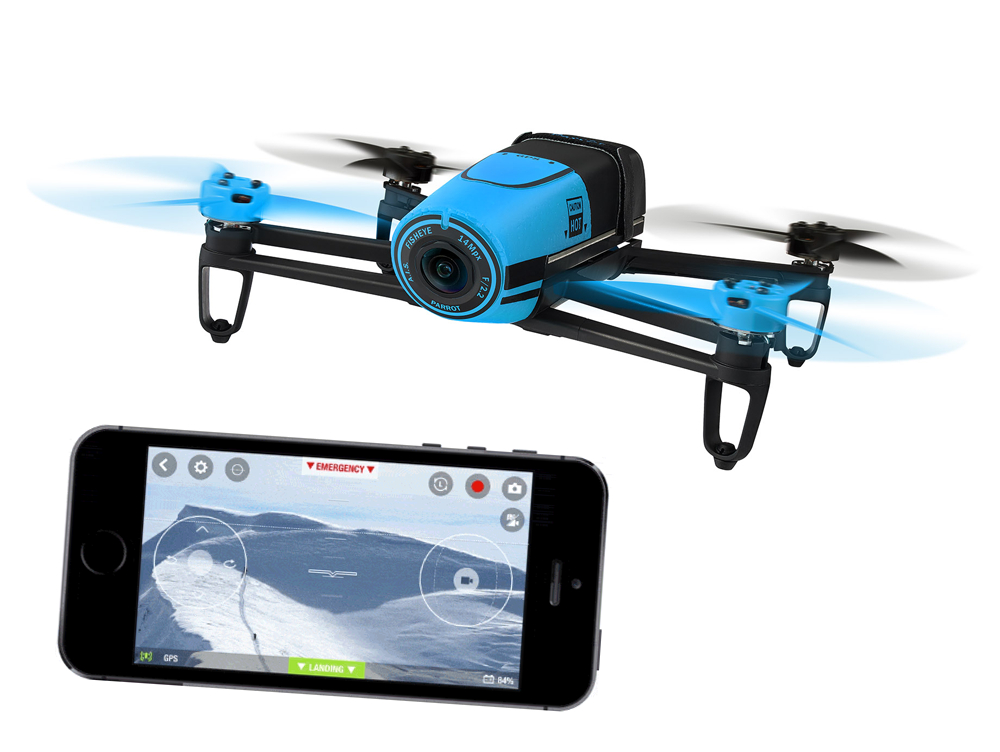
\includegraphics[scale=1]{98_Bilder/04_Anwendungen/parrotdrone}
  \caption[Smartphone gesteuerte Drohne: Parrot bebop]{Parrot bietet Drohnen an, welche mit dem Smartphone gesteuert werden können: Parrot bebop}
  \footnotesize \url{https://s.gravis.de/p/z1/parrot-bebop-drone-kamera-drohne-fuer-smartphones-tablets-gps-blau_z1.jpg}, 04.12.2015
\end{figure}


% Main part - Part V
%---------------------------------------------------------------------------
\onecolumn
\chapter{Technische Anforderungen}
In diesem Kapitel werden die Technischen Voraussetzungen, für die in der Bedürfnisanalyse ermittelten Anwendungen, definiert. Dabei wird unterschieden für Allgemeine Applikationen, welche nur eine kleine Auswahl beachtet wird, und für siot.net Applikationen.

\section{Allgemeine Applikationen Anforderungen}
Die Technischen Anforderungen für die Bedürfnisse Gesundheit, Smart Home und Finanztechnologie werden in diesem Abschnitt definiert.

\subsection{Gesundheit}
Bei den Gesundheitsapplikationen ist es wichtig, dass die Smartwatch über einen Herzfrequenzmesser verfügt und die Kombination aus Gyroskop, Rotationssensor und Bewegungssensor eingebaut ist.
Diese Elemente sind erforderlich um Pulsraten eines Menschen zu messen, sowie Analysen von Bewegungen zu ermitteln.

\textbf{Benötigte Sensoren:}\\
- Gyroskop\\
- Bewegungssensor\\
- Rotationssensor\\
- Herzfrequenzmesser

\subsection{Smart Home}
Für die Steuerung von Haushaltsgeräte, Heizung oder Licht wird vorallem ein Steuerungsanzeige benötigt. Dies ermöglicht die Apparate ein- und auszuschalten, die Beleuchtung zu dimmen und Benachrichtigungen (z.B. von offenem Fenster, beendetem Waschgang uvm.) anzuzeigen. Für eine automatische Helligkeitsregulierung sollte noch ein Lichtmesser eingebaut sein.

\textbf{Bedienelement:}\\
-Touchscreen

\textbf{Benötigter Sensor:}\\
-Lichtsensor

\subsection{Finanztechnologie - FinTech}
Für Geld Transaktionen zu führen wird eine drahtlose Verbindungsart vorausgesetzt. Transaktionen werden Bereits erwähnte Applikationen wie Apple Pay und Google Wallet verwenden den NFC (Near Field Communication) Chip und TWINT verwendet Bluetooth. Die Kommunikationsschnittstelle ist notwendig um Zahlungsanforderungen zu erhalten und diese auch zu authorisieren. Zum auswählen von Zahlungsoptionen und bestätigen von Überweisungen ist ein Bedienelement notwendig. Wenn mehrere Kreditkarten hinterlegt wären, muss der Anwender die Möglichkeit haben, um eine davon auszuwählen für die Überweisung.

\textbf{Auswahl von benötigten Kommunikationsschnittstellen:}\\
- NFC Chip\\
- Bluetooth\\
- GSM/UMTS/LTE\\
- Wireless LAN (weniger geeignet)

\textbf{Mögliche Bedienelemente:}\\
- Touchscreen (beste Vorraussetzung)\\
- Mikrofon zur Sprachsteuerung\\
- Physische Taste\\

\section{siot.net Applikationen Anforderungen}
Technische Voraussetzung für die siot.net Applikationen werden für alle in der Bedürfnisanalyse ermittelten Klassen definiert.

\subsection{siot.net Gateway Library}
Die Bibliothek, welche smarte Geräte an die siot.net Plattform anbinden soll, wird in erster Linie nur für das Android Betriebsystem entwicklet. Für die Benutzung von Apps welche ans siot.net angeschlossen werden, müssen diese minimal die Android Tools der SDK Version 22 beherrschen (ab Android 5.0 Lollipop). Um die Daten an den MQTT Broker übermitteln zu können, braucht es ein Netzwerkmodul, die eine Verbindung ins Internet erlaubt. Die Bibliothek sollte alle verfügbaren und bekannten Sensoren selber erkennen. Die Verwendung, ob Sensoren aktiviert werden oder nicht, wird durch den Appentwickler oder der Software selber definiert.

\textbf{Auswahl von benötigten Kommunikationsschnittstellen:}\\
- NFC Chip\\
- Bluetooth\\
- GSM/UMTS/LTE\\
- Wireless LAN

\textbf{Betriebssystem:}
- ab Android 4.4
- ab SDK Tools Version 22 (Android Tools)

\subsection{siot.net Dashboard App}
Um auch Sensordaten von der siot.net Plattform darzustellen eignet sich eine Dashboard App. Auch diese wird vorraussichtlich nur für Android Geräte implementiert. Für die Darstellung einer derartigen digitalen Instrumententafel eignet sich ein Display, bevorzugt ein Touchscreen. Ein Berührbildschirm erlaubt es die gewünschten Anzeigen bequem einzublenden. Eine weitere Voraussetzung ist die Vernetzung. Das Gerät muss einen Zugang zum Internet herstellen können. Nur durch eine erfolgreiche Anmeldung an den siot.net MQTT Broker, können die Informationen empfangen werden.

\textbf{Auswahl von benötigten Kommunikationsschnittstellen:}\\
- NFC Chip\\
- Bluetooth\\
- GSM/UMTS/LTE\\
- Wireless LAN

\textbf{Bevorzugtes Bedienelement:}\\
- Touchscreen\\

\textbf{Betriebssystem:}
- ab Android 4.4
- ab SDK Tools Version 22 (Android Tools)

\subsection{Herzfrequenz Überwachung}

\subsection{Steuerung von Modellen}
\newpage


% Main part - Part VI
%---------------------------------------------------------------------------
\onecolumn
\chapter{Evaluation Smartwatches}
\section{Aktuell erhältliche}


% Main part - Part VII
%---------------------------------------------------------------------------
\onecolumn
\chapter{Architektur}
\section{Android Wear Paket Architektur}
Android Wear hat eine strikte Paket Architektur. Abbildung 7.1 veranschaulicht die Übersicht diese Architektur. Eine Android Wear App muss immer zwingend eine dazugehörige Android App beinhalten. Wenn beide Apps gemeinsam verwendete Klassen haben, müssen diese in ein solches Paket augelagert werden. Android Klassen können nicht in einer Android Wear Applikation instanziert werden. Üblicherweise wird bei der Installation der .apk auf ein Android Smartphone, parallel die Smartwatch App auf die Uhr mit installiert.
\begin{figure}[h]
  \centering
  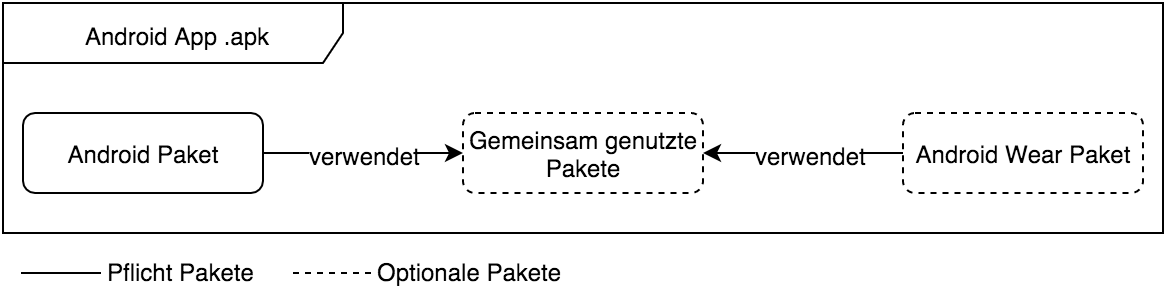
\includegraphics[scale=0.4]{98_Bilder/07_Architektur/AndroidPaketArchitektur}
  \caption[Übersicht Android Wear Paket Architektur]{Übersicht über die einzuhaltende Paketstruktur}
\end{figure}
\section{siot.net Applikationsarchitektur}
Die Architektur auf der Abbildung 7.2 definierte und ersichtliche muss eingehalten. Android und Android Wear Applikation für siot.net können so am effizientesten konzipiert werden.
\begin{figure}[h]
  \centering
  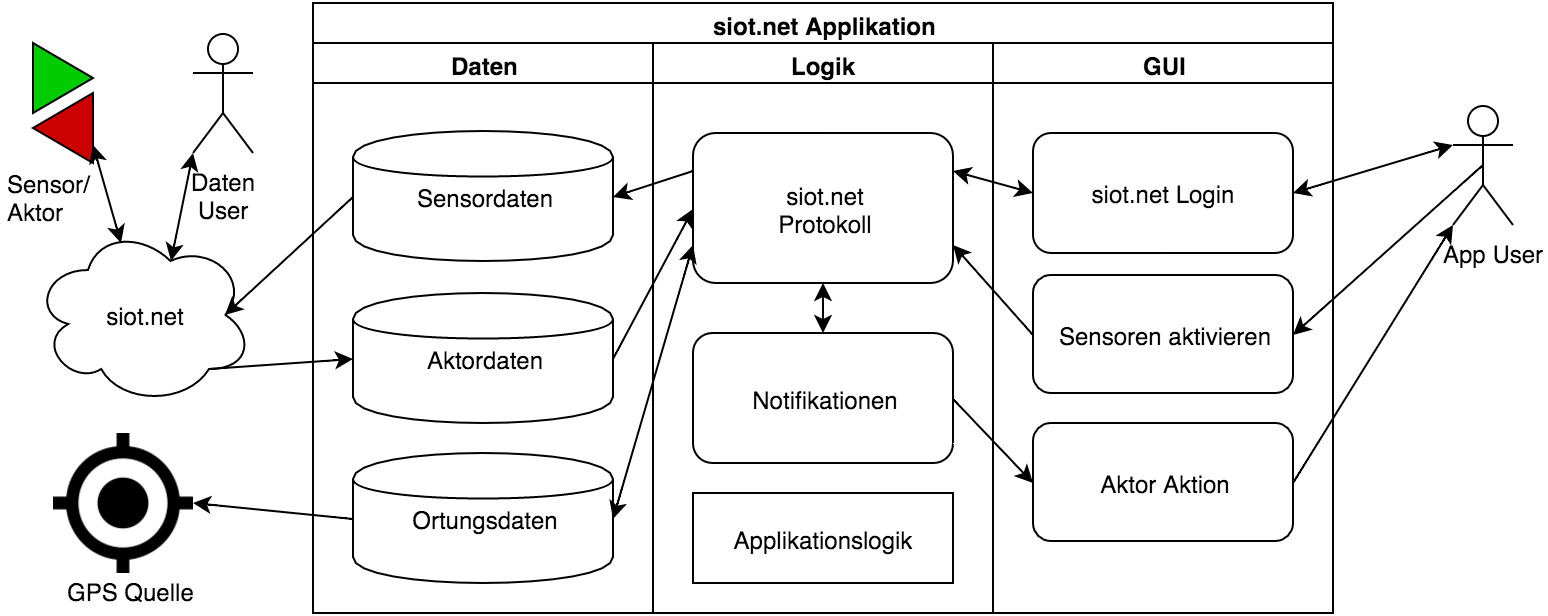
\includegraphics[scale=0.3]{98_Bilder/07_Architektur/siotAppArchitektur}
  \caption[Übersicht siot.net Applikationsarchitektur]{Applikationsarchitektur für siot.net Anwendungen}
\end{figure}
\section{Netzwerk-Architektur}
\subsection{geplante Architektur}
\begin{figure}[h]
  \centering
  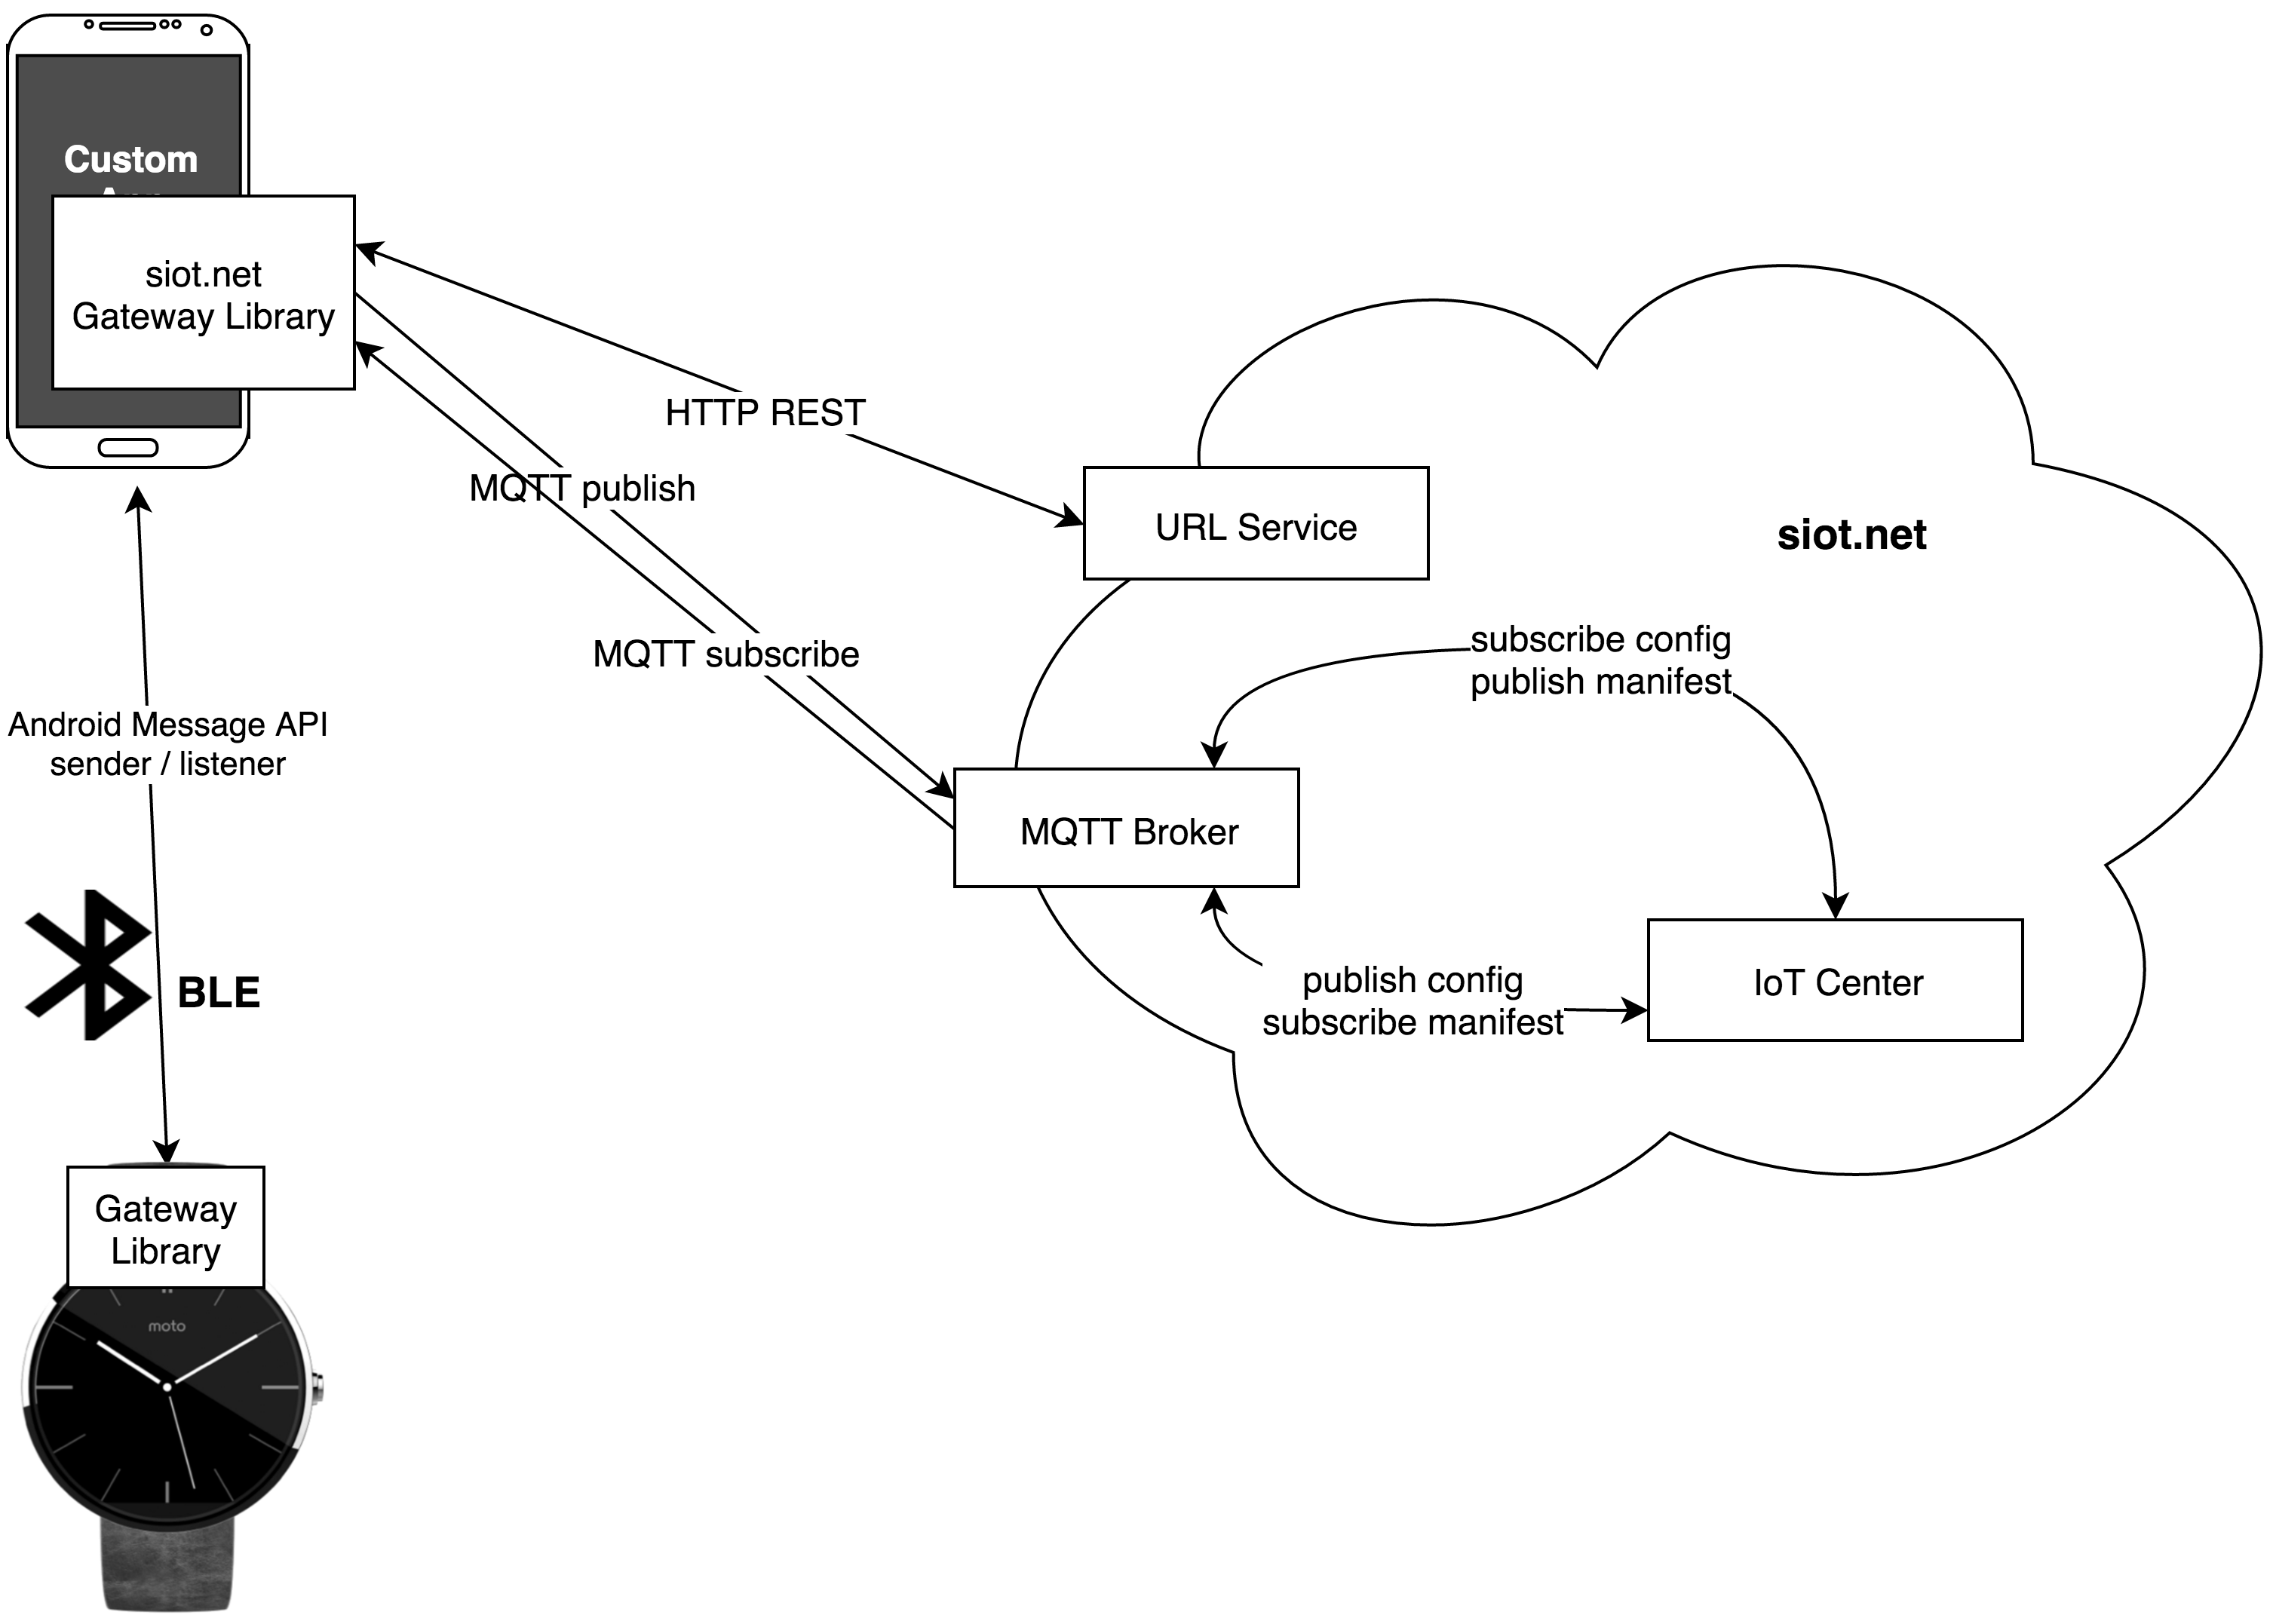
\includegraphics[scale=0.15]{98_Bilder/07_Architektur/01_Architektur}
  \caption[Geplante Netzwerk-Architektur mit BLE/ohne WLAN]{Geplante Kommunikation zwischen Smartwatch und Smartphone, sowie Smartphone und siot.net}
\end{figure}
In der Abbildung 7.3 visualisiert, wie die Kommunikation zwischen der Smartwatch, dem Smartphone und der siot.net Plattform stattfinden soll. Im Falle, dass die Smartwatch eine Bluetooth Low Energy (BLE) Verbindung mit dem Smartphone aufweist, wird dieses via REST und MQTT, mit siot.net Daten austauschen. Dabei dient das Mobiltelefon als Datenbrücke von der Smartwatch zur IoT-Cloud. Die Android Wear Uhr versendet die Daten, per Android Message API via BLE, zum Android Smartphone, das leitet die Pakete mit Hilfe des MQTT Protokoll weiter ans siot.net. Diese Variante der Datenübermittlung ist sehr viel stromsparender als die in Abbildung 7.4 gezeigte.\\
Das Bridging muss in der Smartphone Begleitapp (Android Paket) der Smartwatch Applikation (Android Wear Paket) implementiert sein.
\newpage
\begin{figure}[h]
  \centering
  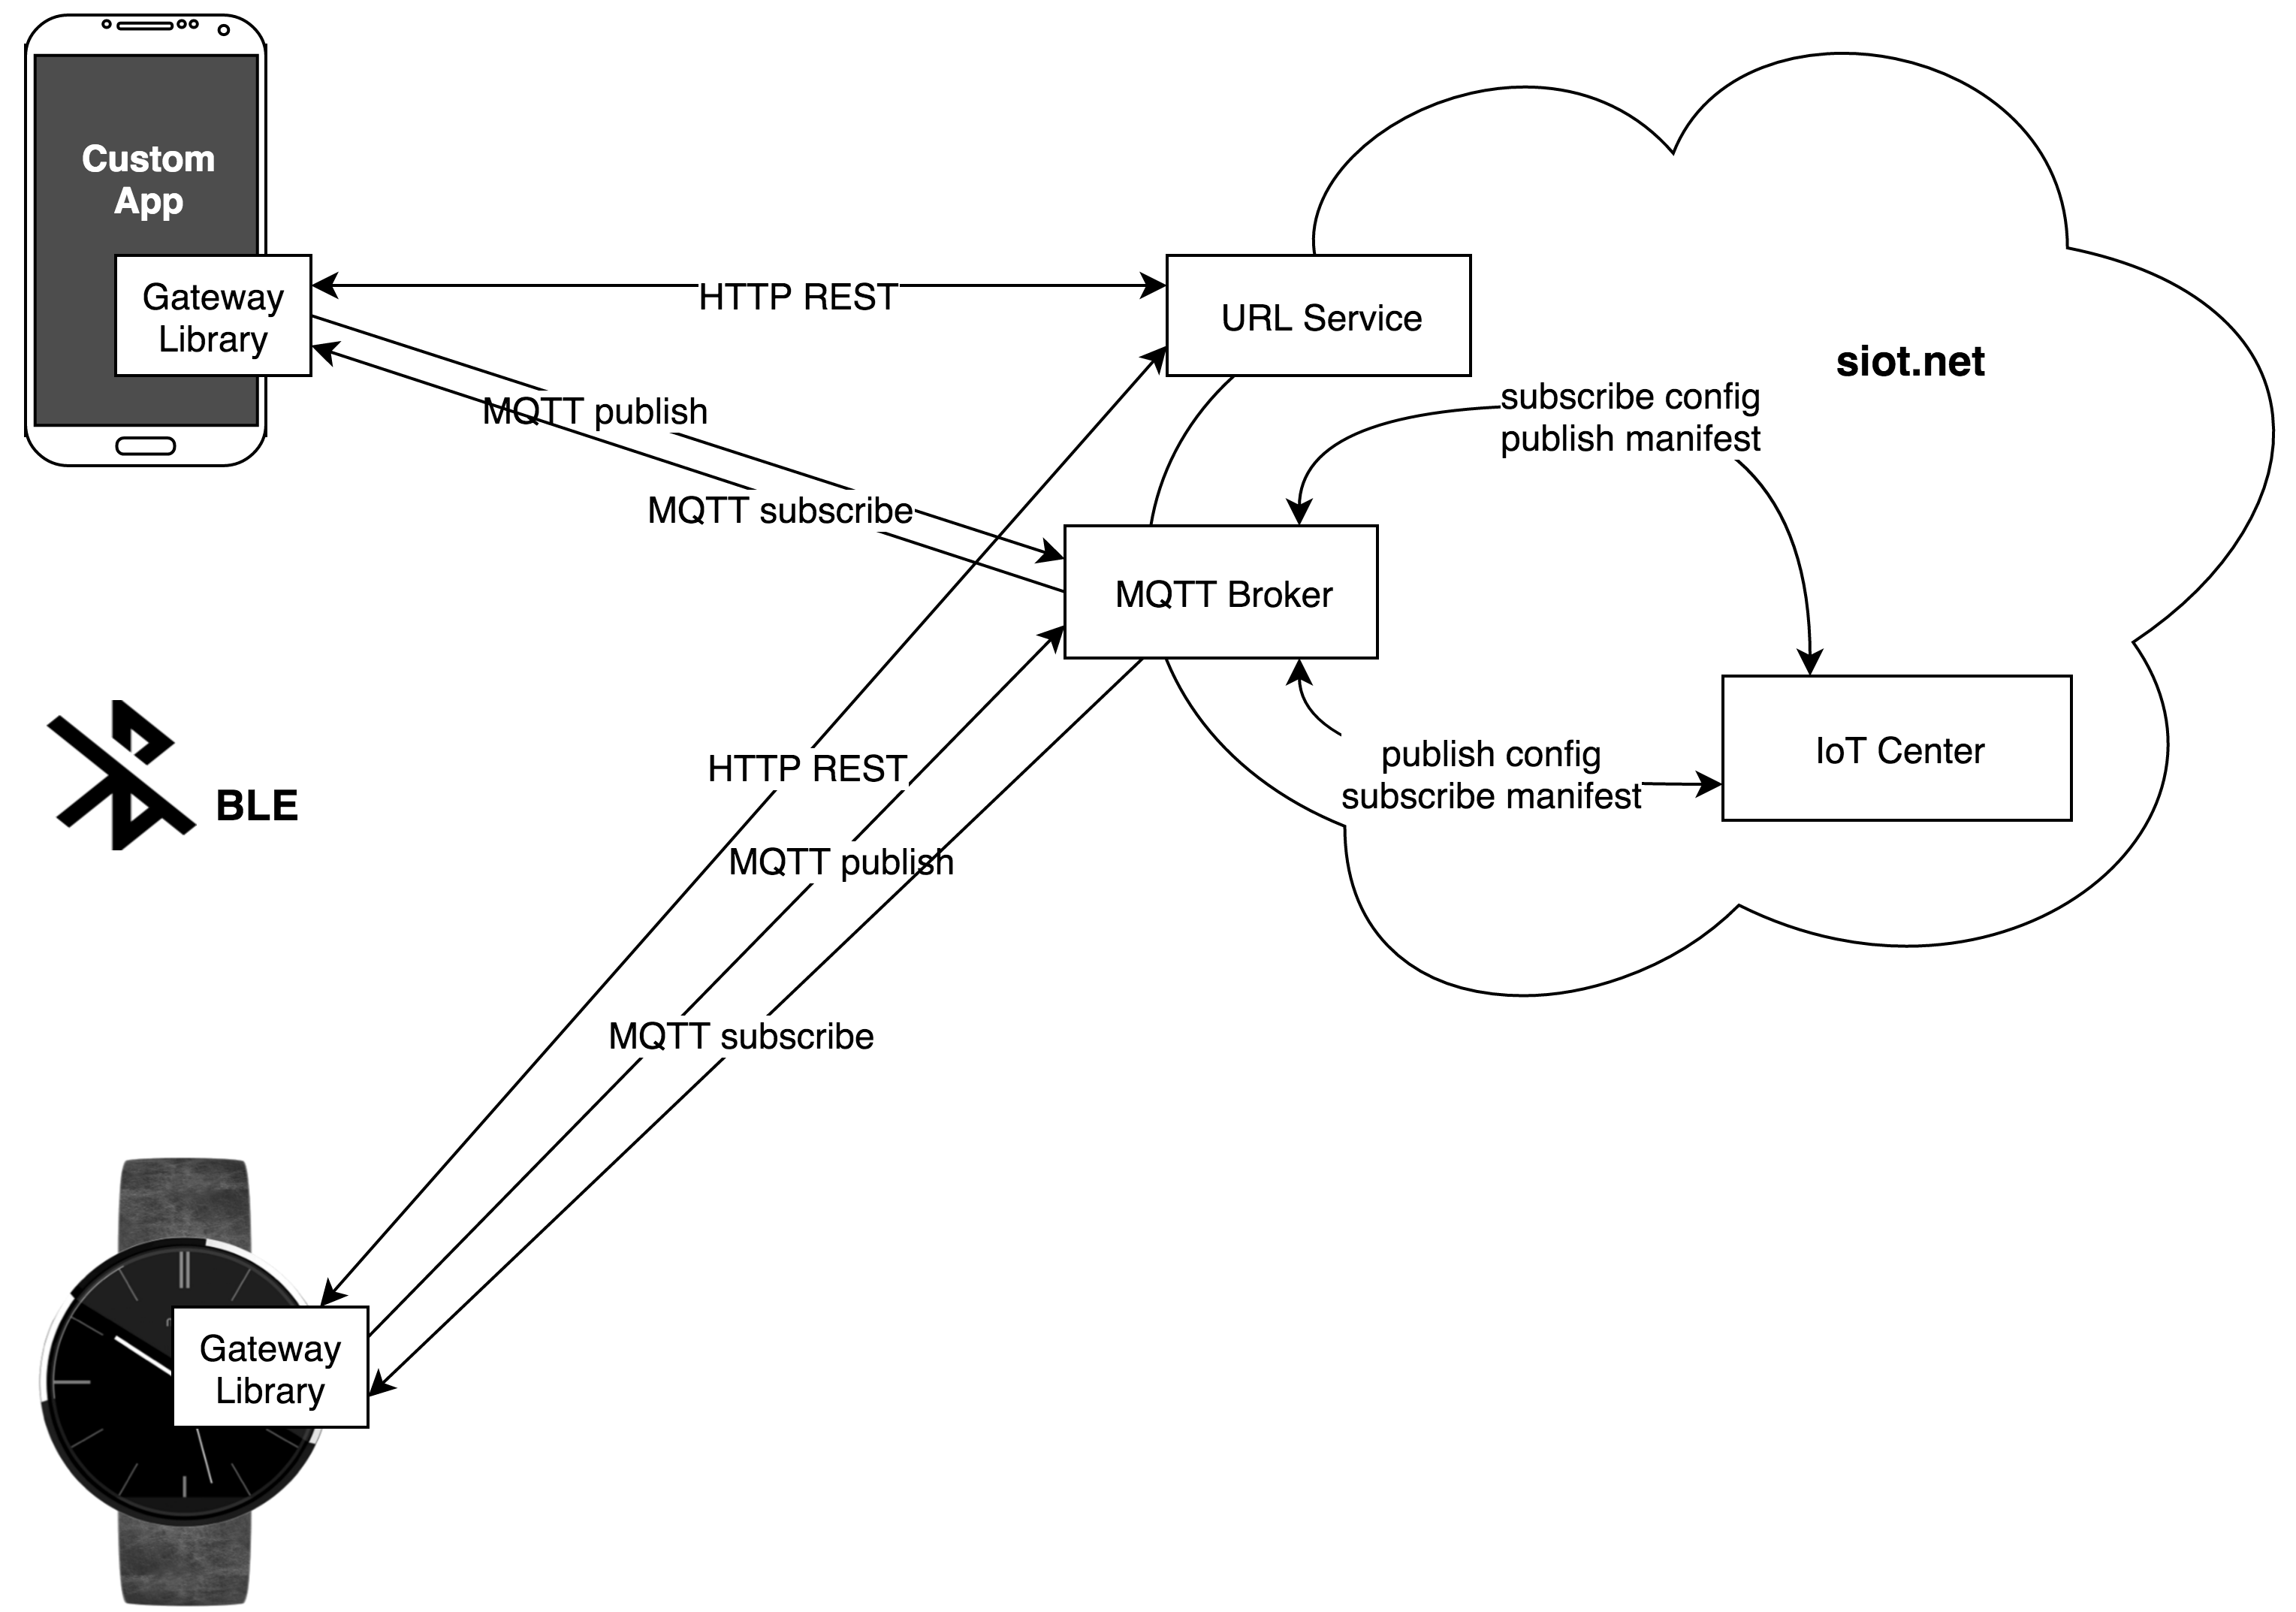
\includegraphics[scale=0.15]{98_Bilder/07_Architektur/02_Architektur}
  \caption[Geplante Netzwerk-Architektur ohne BLE/mit WLAN]{Geplante Kommunikation zwischen Smartwatch und siot.net, sowie Smartphone und siot.net}
\end{figure}
Bei Abbruch der Verbindung von Smartwatch zu Smartphone, soll die Computeruhr die Kommunikation zum siot.net selber übernehmen. Dazu muss zuerst über REST die URL des MQTT Broker ermittelt werden, um folgliche eine Kopplung durchzuführen. Diese Architektur ist genauer auf Abbildung 7.4 zu betrachten.

\newpage
\subsection{effektive Architektur}
\begin{figure}[h]
  \centering
  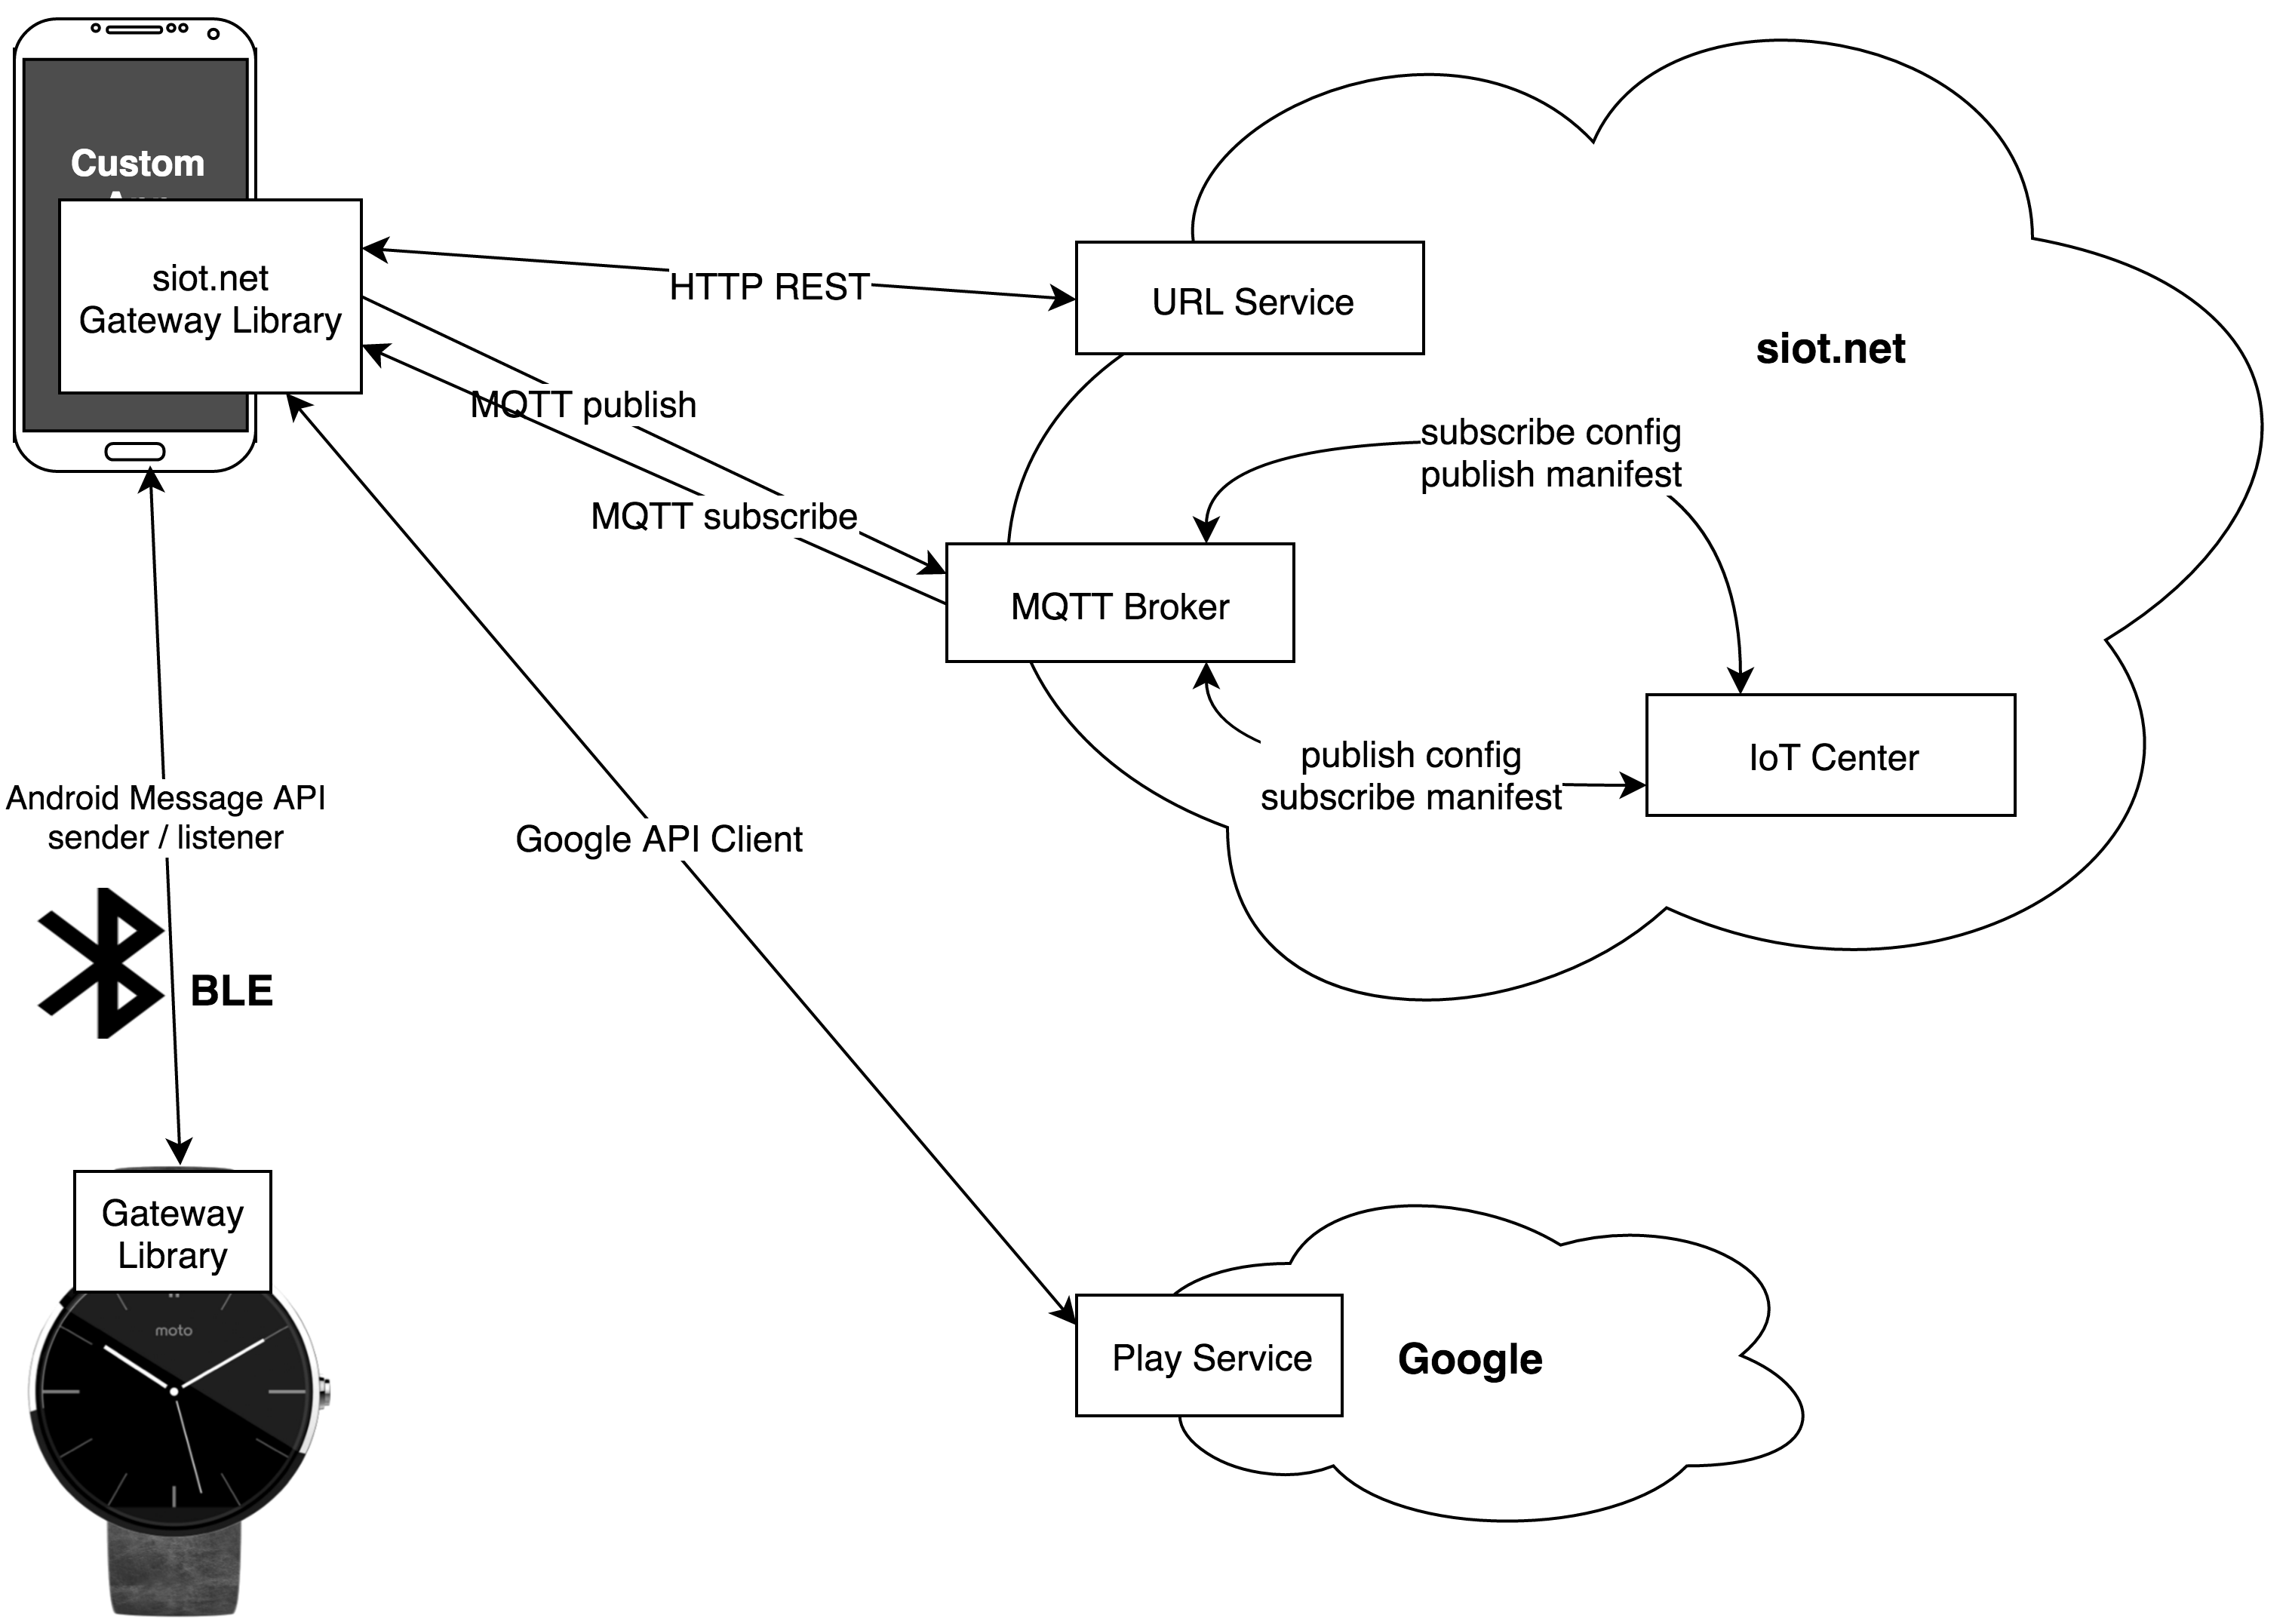
\includegraphics[scale=0.15]{98_Bilder/07_Architektur/03_Architektur}
  \caption[Effektive Netzwerk-Architektur mit BLE/ohne WLAN]{Effektive Kommunikation zwischen Smartwatch und siot.net, sowie Smartphone und siot.net}
\end{figure}
Diese Architektur (siehe Abbildung 7.5) unterscheidet sich geringfügig zu jener Abbildung 7.3. Hier kommt nun die Google Cloud dazu. Dies ist notwendig, da Android nicht erlaubt direkt über die Android Message API zu kommunizieren. Es muss vorhergehend eine NodeId über den Google Play Service eingefordert werden. Dank dieser NodeId dürfen die Geräte (Smartphone und Smartwatch benötigen eine eindeutige Identifikation) mittels Message API Nachrichten transferieren. Der Datenaustausch geschieht dann direkt via BLE. Dies ist die Netzwerk-Architektur kommt zum tragen, wenn die Kopplung von Smartwatch und Smartphone über Bluetooth Smart steht.

\newpage
\begin{figure}[h]
  \centering
  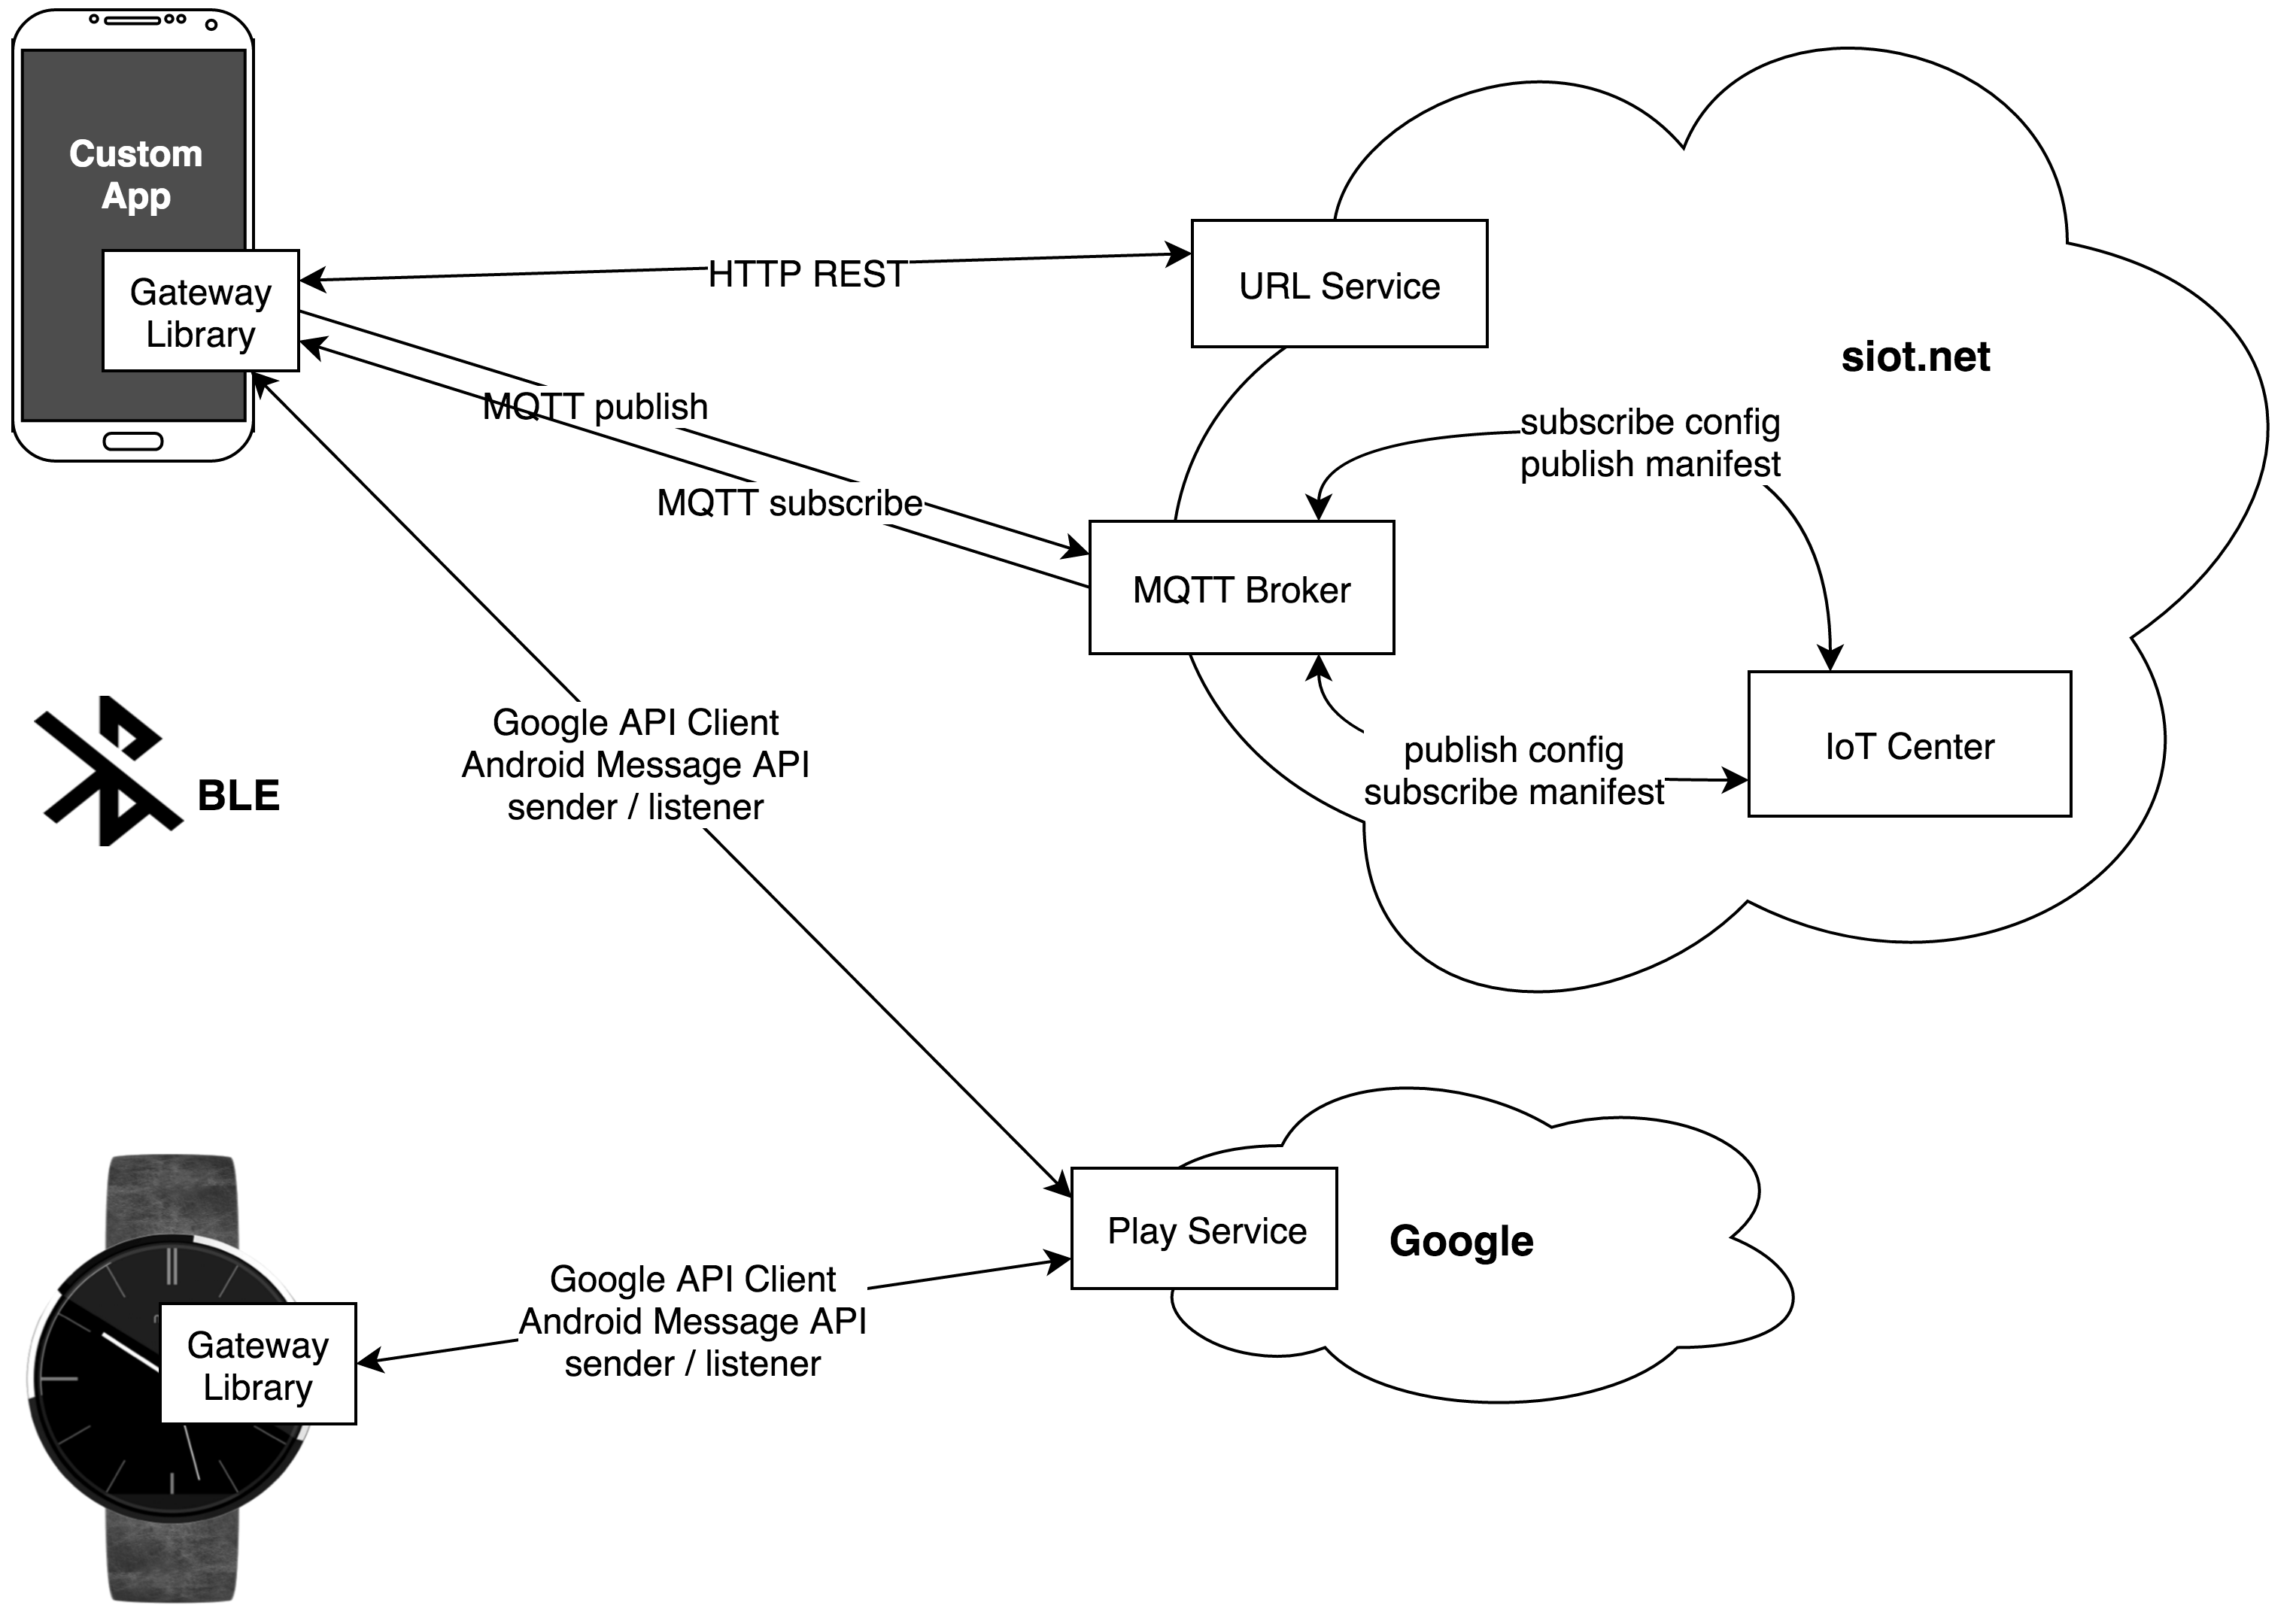
\includegraphics[scale=0.15]{98_Bilder/07_Architektur/04_Architektur}
  \caption[Effektive Netzwerk-Architektur mit BLE/ohne WLAN]{Effektive Kommunikation zwischen Smartwatch und siot.net, sowie Smartphone und siot.net}
\end{figure}
Abbildung 7.6 zeigt die funktionierende Architektur. Diese differenziert sich wesentlich von der geplanten Netzwerk-Definition. Auch hier spielt der Faktor Android eine grosse Rolle, denn es verbietet Android Wear Geräten den direkten Kontakt zum Internet. So ist hier eine Verbindung über den Google Play Service zum Smartphone nötig. Bei dieser Anbindungsart werden die Daten via Google Cloud an das Android Handy gesendet. Es muss in jedemfall die Verbindung zu siot.net verwalten.\\
Der grosse Nachteil dieser Variante ist, dass die Smartwatch nicht als autonomes Gerät fungieren kann. Wenn das Smartphone nicht erreichbar ist, z.B. Akku leer, keine Netzverbindung, ist die Smartwatch für siot.net nutzlos.


% Main part - Part VIII
%---------------------------------------------------------------------------
\onecolumn
\chapter{Anforderungsdokumente}
Dieser Teil des Dokuments beinhaltet drei Anforderungsdokumente von der vorhergehend ermittelten Anwendungen.
Requirements von der siot.net Gateway Library, siot.net Sensorcenter und siot.net Dashboard App sind aufgeführt.
\section{Requirements - siot.net Gateway Library}
In diesem Requirementsdokument werden die Anforderung an die siot.net Gateway Library \textbf{(sGWLib)} spezifizert.
\subsection{Allgemeine Beschreibung}
Die siot.net Gateway Library soll Entwicklern von Android Apps für Mobile Geräte, wie Smartphones oder Smartwatches, erleichtern Ihre Software an die siot.net Plattform anzubinden.
Programmieren von Applikationen muss immer eifacher und schneller werden, da Projekte immer mehr an höherem Zeitdruck leiden. Diese Bibliothek soll helfen Integrationen von Apps an das siot.net ohne grosses Vorwissen, schnell durchzuführen.
Die Library übernimmt die Verwaltung von den Sensor den Gerätes, sowie die Kommunikation von Mobile Device zu siot.net und Smartwatch zu Smartphone.
\subsection{User Requirements}
\begin{figure}[h]
  \centering
  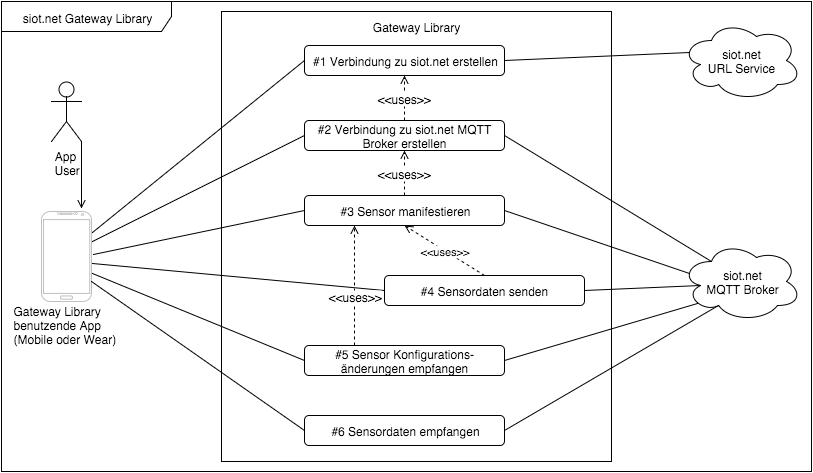
\includegraphics[scale=0.6]{98_Bilder/08_Requirements/UseCaseGatewayLibrary}
  \caption[Use Case siot.net Gateway Library]{Das allgemeine Use Case Diagramm für die siot.net Gateway Library}
\end{figure}

\subsection{Funktionale Anforderungen und Anwendungsfallbeschreibungen}
\subsubsection{Anwendungsfall \#1}
\begin{table}[H]
\centering
\begin{tabular}{|>{\columncolor[gray]{0.8}}l|p{11.5cm}|}
\hline
\textbf{Nr. und Name:}                  & \#1 Verbindung zu siot.net erstellen. \\ \hline
\textbf{Szenario:}                      & Android Gerät wird mit dem siot.net verbunden. \\ \hline
\textbf{Kurzbeschreibung:}              & Die Verbindung des Android Devices zum siot.net wird hergestellt, dies geschieht über den URL Service um die nötigen URLs zu erhalten (IoT Center und MQTT Broker). \\ \hline
\textbf{Beteiligt Akteure:}             & Android App (User), siot.net Gateway Library, siot.net URL Service, siot.net MQTT Broker. \\ \hline
\textbf{Auslöser und Vorbedingung:}     & User gibt über seine App den Befehl zu die Applikation zu einer IoT Cloud zu verbinden. Wenn siot.net als Ziel gewählt wird, muss die siot.net Gateway Library eingebunden sein. Für eine erfolgreiche Verbindung muss eine gültige siot.net Lizenz vorhanden sein. \\ \hline
\textbf{Ergebnisse und Nachbedingung:}  & Der URL Service von siot.net kann die Lizenz richtig verifizieren und liefert die benötigten URLs. \\ \hline
\end{tabular}
\caption{siot.net Gateway Library: Übersicht Anwendungsfall \#1}
\end{table}
\textbf{Ablauf:}
\begin{table}[H]
\centering
\begin{tabular}{|>{\columncolor[gray]{0.8}}p{1.3cm}|p{1.7cm}|p{13.2cm}|}
\hline
\textbf{1-1}  & App User    & Startet die App. \\ \hline
\textbf{1-2}  & App User    & Gibt siot.net Lizenz ein und klickt verbinden zu siot.net. \\ \hline
\textbf{1-3}  & App         & Forder bei der siot.net Gateway Library (sGWLib) die Verbindung an. \\ \hline
\textbf{1-4}  & sGWLib      & Verfiziert sich beim siot.net URL Service mit dem Lizenzschlüssel. \\ \hline
\textbf{1-5}  & sGWLib      & Erhält URL vom siot.net MQTT Broker und verbindet sich (Anwendungsfall \#2). \\ \hline
\textbf{1-6}  & sGWLib      & App über Verbindungsstatus benachrichtigen. \\ \hline
\textbf{1-7}  & App         & Benachrichtigung verarbeiten, z.B. Meldung an App User. \\ \hline
\end{tabular}
\caption{siot.net Gateway Library: Chronologischer Ablauf von Anwendungsfall \#1}
\end{table}
\textbf{Ausnahmen und Varianten:}
\begin{table}[H]
\centering
\begin{tabular}{|>{\columncolor[gray]{0.8}}p{1.3cm}|p{1.7cm}|p{13.2cm}|}
\hline
\textbf{1-4.1}  & sGWLib     & Ausnahme: siot.net URL Service nicht erreichbar, App benachrichtigen. \\ \hline
\textbf{1-4.2}  & sGWLib     & Ausnahme: Lizenzschlüssel nicht valide, App benachrichtigen. \\ \hline
\textbf{1-5.1}  & sGWLib     & Ausnahme: MQTT Broker nicht erreichbar, App benachrichtigen. \\ \hline
\end{tabular}
\caption{siot.net Gateway Library: Ausnahmen und Varianten von Anwendungsfall \#1}
\end{table}

\newpage

\subsubsection{Anwendungsfall \#2}
\begin{table}[H]
\centering
\begin{tabular}{|>{\columncolor[gray]{0.8}}l|p{11.5cm}|}
\hline
\textbf{Nr. und Name:}                  & \#2 Verbindung zu siot.net MQTT Broker erstellen. \\ \hline
\textbf{Szenario:}                      & Verbindung zum siot.net MQTT Broker herstellen. \\ \hline
\textbf{Kurzbeschreibung:}              & Durch die vom URL Service erhaltene MQTT URL wird das Android Gerät wird mit dem Broker gekoppelt. \\ \hline
\textbf{Beteiligt Akteure:}             & siot.net Gateway Library, siot.net URL Service, siot.net MQTT Broker. \\ \hline
\textbf{Auslöser und Vorbedingung:}     & Durch das erhalten einer gültigen MQTT Broker URL wird der Verbindungsversuch gestartet. \\ \hline
\textbf{Ergebnisse und Nachbedingung:}  & Es kann erfolgreich ein MQTT Client Verbindung produziert werden. \\ \hline
\end{tabular}
\caption{siot.net Gateway Library: Übersicht Anwendungsfall \#2}
\end{table}
\textbf{Ablauf:}
\begin{table}[H]
\centering
\begin{tabular}{|>{\columncolor[gray]{0.8}}p{1.3cm}|p{1.7cm}|p{13.2cm}|}
\hline
\textbf{2-1}  & sGWLib  & Empfang der URLs vom siot.net URL Service. \\ \hline
\textbf{2-2}  & sGWLib  & MQTT URL wird verwendet um eine Verbindung zum Broker aufzubauen. \\ \hline
\textbf{2-3}  & sGWLib  & Verbindungsstatus wird überprüft und stellt die Verbindungsinstanz der App zur Verfügung. \\ \hline
\end{tabular}
\caption{siot.net Gateway Library: Chronologischer Ablauf von Anwendungsfall \#2}
\end{table}
\textbf{Ausnahmen und Varianten:}
\begin{table}[H]
\centering
\begin{tabular}{|>{\columncolor[gray]{0.8}}p{1.3cm}|p{1.7cm}|p{13.2cm}|}
\hline
\textbf{2-2.1}  & sGWLib     & Ausnahme: Authentifizierung fehlgeschlagen - Lizenzschlüssel ungültig, App benachrichtigen. \\ \hline
\textbf{2-2.2}  & sGWLib     & Ausnahme: Keine MQTT Broker URL erhalten, Information an App senden. \\ \hline
\textbf{2-2.3}  & sGWLib     & Ausnahme: MQTT Broker nicht erreichbar, App benachrichtigen. \\ \hline
\textbf{2-2.4}  & sGWLib     & Variante: Mehrere MQTT Broker URLs erhalten, absteigend der Reihe nacheinander Verbindungsversuche starten bei erstem Erfolg diesen Client verwenden und der App zur Verfügung stellen. \\ \hline
\end{tabular}
\caption{siot.net Gateway Library: Ausnahmen und Varianten von Anwendungsfall \#2}
\end{table}

\newpage

\subsubsection{Anwendungsfall \#3}
\begin{table}[H]
\centering
\begin{tabular}{|>{\columncolor[gray]{0.8}}l|p{11.5cm}|}
\hline
\textbf{Nr. und Name:}                  & \#3 Sensor manifestieren. \\ \hline
\textbf{Szenario:}                      & Manifestieren vom gewünschten Sensor beim siot.net \\ \hline
\textbf{Kurzbeschreibung:}              & Jeder Sensor welcher an die siot.net Plattform angebunden wird, muss sich zuerst manifestieren. Dies geschieht durch eine MQTT Meldung, des Datentyps Manifest (definiert durch siot.net), an den siot.net Broker. \\ \hline
\textbf{Beteiligt Akteure:}             & siot.net Gateway Library, siot.net MQTT Broker. \\ \hline
\textbf{Auslöser und Vorbedingung:}     & Wenn die App zum ersten Mal eine App ans siot.net anmelden will und dieser nicht dem IoT Center nicht bekannt ist. \\ \hline
\textbf{Ergebnisse und Nachbedingung:}  & Der Sensor kann erfolgreich am IoT Center von siot.net manifestiert und danach verwaltet werden. \\ \hline
\end{tabular}
\caption{siot.net Gateway Library: Übersicht Anwendungsfall \#3}
\end{table}
\textbf{Ablauf:}
\begin{table}[H]
\centering
\begin{tabular}{|>{\columncolor[gray]{0.8}}p{1.3cm}|p{1.7cm}|p{13.2cm}|}
\hline
\textbf{3-1}  & App     & App meldet einen Sensor zur Anmeldung am siot.net dem siot.net Gateway Library. \\ \hline
\textbf{3-2}  & sGWLib  & Sensor wird instanziert, eindeutige GUID wird generiert und Manifest wird erstellt. \\ \hline
\textbf{3-3}  & sGWLib  & Manifest wird an siot.net MQTT Broker gesendet. \\ \hline
\textbf{3-4}  & sGWLib  & Gateway Library abonniert die Konfigurationstopic des MQTT Brokers des manifestierten Sensors. \\ \hline
\textbf{3-5}  & sGWLib  & Sensor ist nun für die App bereitgestellt. \\ \hline
\end{tabular}
\caption{siot.net Gateway Library: Chronologischer Ablauf von Anwendungsfall \#3}
\end{table}
\textbf{Ausnahmen und Varianten:}
\begin{table}[H]
\centering
\begin{tabular}{|>{\columncolor[gray]{0.8}}p{1.3cm}|p{1.7cm}|p{13.2cm}|}
\hline
\textbf{3-3.1}  & sGWLib     & Ausnahme: MQTT Verbindung nicht verfügbar, App informieren. \\ \hline
\textbf{3-2.1}  & sGWLib     & Variante: Gemeldete Sensor verwaltet mehrere physische Werte, pro Angabe wird ein Sensormanifest angelegt. \\ \hline
\textbf{3-2.2}  & sGWLib     & Variante: Sensor ist dem siot.net IoT Center bereits bekannt, es wird kein neuer Sensor angelegt sondern als bereits verfügbaren registriert, keine Aktion notwendig. \\ \hline
\end{tabular}
\caption{siot.net Gateway Library: Ausnahmen und Varianten von Anwendungsfall \#3}
\end{table}

\newpage

\subsubsection{Anwendungsfall \#4}
\begin{table}[H]
\centering
\begin{tabular}{|>{\columncolor[gray]{0.8}}l|p{11.5cm}|}
\hline
\textbf{Nr. und Name:}                  & \#4 Sensordaten senden. \\ \hline
\textbf{Szenario:}                      & Sensorwerte an den siot.net MQTT Broker senden. \\ \hline
\textbf{Kurzbeschreibung:}              & Sensordaten werden vom Datentyp Sensordaten (spezifiziert von siot.net) an den Broker per MQTT gesendet. \\ \hline
\textbf{Beteiligt Akteure:}             & Android System, siot.net Gateway Library, siot.net MQTT Broker. \\ \hline
\textbf{Auslöser und Vorbedingung:}     & Sensor meldet, dass neue Daten verfügbar sind. \\ \hline
\textbf{Ergebnisse und Nachbedingung:}  & Werte können mit Erfolg an den MQTT broker publiziert werden. \\ \hline
\end{tabular}
\caption{siot.net Gateway Library: Übersicht Anwendungsfall \#4}
\end{table}
\textbf{Ablauf:}
\begin{table}[H]
\centering
\begin{tabular}{|>{\columncolor[gray]{0.8}}p{1.3cm}|p{1.7cm}|p{13.2cm}|}
\hline
\textbf{4-1}  & Android  & Sensor meldet an, dass neue Werte ermittelt wurden. \\ \hline
\textbf{4-2}  & sGWLib  & Sensordaten Datentyp wird angefertigt. \\ \hline
\textbf{4-3}  & sGWLib  & Sensordaten Meldung wird an siot.net MQTT Broker gesendet. \\ \hline
\end{tabular}
\caption{siot.net Gateway Library: Chronologischer Ablauf von Anwendungsfall \#4}
\end{table}
\textbf{Ausnahmen und Varianten:}
\begin{table}[H]
\centering
\begin{tabular}{|>{\columncolor[gray]{0.8}}p{1.3cm}|p{1.7cm}|p{13.2cm}|}
\hline
\textbf{4-3.1}  & sGWLib   & Ausnahme: MQTT Verbindung nicht verfügbar, App informieren. \\ \hline
\end{tabular}
\caption{siot.net Gateway Library: Ausnahmen und Varianten von Anwendungsfall \#4}
\end{table}

\newpage

\subsubsection{Anwendungsfall \#5}
\begin{table}[H]
\centering
\begin{tabular}{|>{\columncolor[gray]{0.8}}l|p{11.5cm}|}
\hline
\textbf{Nr. und Name:}                  & \#5 Sensor Konfigurationsänderung empfangen. \\ \hline
\textbf{Szenario:}                      & Konfigurationsänderungen im siot.net IoT Center empfangen und verarbeiten. \\ \hline
\textbf{Kurzbeschreibung:}              & Sensoren werden im siot.net IoT Center verwaltet und konfiguriert. Bei der Änderung einer Einstellung wird der Sensor per MQTT Message notifiziert. Die Gateway Library empfängt die Nachricht und stellt den Sensor den Werten entsprechend ein. \\ \hline
\textbf{Beteiligt Akteure:}             & siot.net Gateway Library, siot.net MQTT Broker. \\ \hline
\textbf{Auslöser und Vorbedingung:}     & Konfigurationsnachricht von siot.net MQTT Broker erhalten. \\ \hline
\textbf{Ergebnisse und Nachbedingung:}  & Sensor kann korrekt umkonfiguriert werden. \\ \hline
\end{tabular}
\caption{siot.net Gateway Library: Übersicht Anwendungsfall \#5}
\end{table}
\textbf{Ablauf:}
\begin{table}[H]
\centering
\begin{tabular}{|>{\columncolor[gray]{0.8}}p{1.3cm}|p{1.7cm}|p{13.2cm}|}
\hline
\textbf{5-1}  & sGWLib  & Erhält Message mit neuen Sensoreinstellungen. \\ \hline
\textbf{5-2}  & sGWLib  & Konfiguration wird geparsed und einem Sensor zugeordnet. \\ \hline
\textbf{5-3}  & sGWLib  & Sensor wird umkonfiguriert. \\ \hline
\end{tabular}
\caption{siot.net Gateway Library: Chronologischer Ablauf von Anwendungsfall \#5}
\end{table}
\textbf{Ausnahmen und Varianten:}
\begin{table}[H]
\centering
\begin{tabular}{|>{\columncolor[gray]{0.8}}p{1.3cm}|p{1.7cm}|p{13.2cm}|}
\hline
\textbf{5-3.1}  & sGWLib   & Variante: Konfiguration ist einem physischen Werte eines Sensor zugeordenet, welcher mehrere verwaltet, gesammten Sensor neu einstellen. Weiteres verhalten muss in einem neuen Projekt genauer definiert werden (Sensorkombinationen sind im siot.net vorgesehen, jedoch noch nicht spezifiziert und freigegeben). \\ \hline
\end{tabular}
\caption{siot.net Gateway Library: Ausnahmen und Varianten von Anwendungsfall \#5}
\end{table}

\newpage

\subsubsection{Anwendungsfall \#6}
\begin{table}[H]
\centering
\begin{tabular}{|>{\columncolor[gray]{0.8}}l|p{11.5cm}|}
\hline
\textbf{Nr. und Name:}                  & \#6 Sensordaten empfangen. \\ \hline
\textbf{Szenario:}                      & Sensordaten von anderen Sensoren im siot.net empfangen und bereitstellen. \\ \hline
\textbf{Kurzbeschreibung:}              & Die siot.net Gateway Library kann auch Sensordaten empfangen welche beim siot.net IoT Center angemeldet sind. Sensordaten können beim MQTT Broker subskribiert werden. Beim Empfang einer Informationennachricht wird diese interpretiert und der App zur Verwendung gestellt. \\ \hline
\textbf{Beteiligt Akteure:}             & siot.net Gateway Library, siot.net MQTT Broker. \\ \hline
\textbf{Auslöser und Vorbedingung:}     & Sensordaten Message von siot.net MQTT Broker erhalten. \\ \hline
\textbf{Ergebnisse und Nachbedingung:}  & Informationen sind interpretiert und verfügbar gemacht. \\ \hline
\end{tabular}
\caption{siot.net Gateway Library: Übersicht Anwendungsfall \#6}
\end{table}
\textbf{Ablauf:}
\begin{table}[H]
\centering
\begin{tabular}{|>{\columncolor[gray]{0.8}}p{1.3cm}|p{1.7cm}|p{13.2cm}|}
\hline
\textbf{6-1}  & sGWLib  & Erhält Message mit Sensordaten. \\ \hline
\textbf{6-2}  & sGWLib  & Infomationen interpretieren. \\ \hline
\textbf{6-3}  & sGWLib  & Datenzugriff der App erlauben. \\ \hline
\end{tabular}
\caption{siot.net Gateway Library: Chronologischer Ablauf von Anwendungsfall \#6}
\end{table}
\textbf{Ausnahmen und Varianten:}
\begin{table}[H]
\centering
\begin{tabular}{|>{\columncolor[gray]{0.8}}p{1.3cm}|p{1.7cm}|p{13.2cm}|}
\hline
\textbf{6-2.1}  & sGWLib   & Ausnahme: Empfangene Nachricht kann nicht interpretiert werden als Sensordaten, Information wird verworfen. \\ \hline
\end{tabular}
\caption{siot.net Gateway Library: Ausnahmen und Varianten von Anwendungsfall \#6}
\end{table}

\subsection{Nicht-funktionale Anforderungen}
\textbf{Produktanforderungen:}
\begin{table}[H]
\centering
\begin{tabular}{|>{\columncolor[gray]{0.8}}p{5cm}|p{11.5cm}|}
\hline
\textbf{Benutzbarkeitsanforderungen}    & Die Bibliothek muss eine Java Library sein, um diese möglichst eifach in ein Android Projekt integrieren zu können. \\ \hline
\textbf{Effizienzanforderungen}         & Ein übersichtiliche und schlanke Dokumentation (z.B. JavaDoc oder Entwicklerhandbuch) soll dem Entwickler helfen, eine neue App zu programmieren. \\ \hline
\textbf{Zuverlässigkeitsanforderungen}  & Die Daten, welche transferiert werden, verwenden das fire-and-forget Entwicklungsdesignmuster. Bei diesem Muster werden die gesendeten Nachrichten nicht mehr verfolgt. Wenn eine Message nicht ankommt, wird dies von keinem System bemerkt. Da Daten nur durch den vom Benutzer gewünschten Sensoren versendet werden, vereifach dieses Pattern die Kommunikation zwischen Smartdevice und siot.net. Der Sicherheitsaspekt wird in einem weiteren Release verfolgt. Technisch sollte die Applikation, die vorhandene Hardware nicht überfordern. \\ \hline
\textbf{Portierbarkeitsanforderungen}   & Die Informationen werden in einem Format übertragen und empfangen wie sie von siot.net spezifiziert sind. \\ \hline
\textbf{Performanceanforderung}         & An die Performance sind keine spezifischen Anforderungen gestellt. Daten sollten in nützlicher Frist gesendet werden {(z.B. <5 Sekunden Verzögerung pro Nachricht)} \\ \hline
\end{tabular}
\caption{siot.net Gateway Library: Nicht-funktionale Produktanforderungen}
\end{table}

\newpage

\section{Requirements - siot.net Sensorcenter}
In diesem Requirementsdokument werden die Anforderung an die Android App siot.net Sensorcenter Android \textbf{(sSC-A)} und siot.net Sensorcenter Android Wear \textbf{(sSC-AW)} spezifizert.
\subsection{Allgemeine Beschreibung}
Das siot.net Sensorcenter für Android Geräte, ist die erste Applikation welche die siot.net Gateway Library (sGWLib) integrieren soll. Ein Android Device eignet sich sehr gut als eigenes Sensorcenter, weil die mobilen Telefone und Uhren haben grosse Mengen von Sensoren eingebaut. Diese App bietet die Möglichkeit alle vom User gewünschten Sensordaten dem siot.net preiszugeben. Der Benutzer kann die Sensoren selber aktivieren und deaktivieren. Die gemessenen Daten werden via MQTT, mit Hilfe der siot.net Gateway Library, übermittelt.
\subsection{User Requirements}
\begin{figure}[h]
  \centering
  \includegraphics[scale=0.42]{98_Bilder/08_Requirements/UseCaseSensorcenter}
  \caption[Use Case siot.net Sensorcenter]{Das allgemeine Use Case Diagramm für das siot.net Sensorcenter}
\end{figure}
\newpage
\subsection{Funktionale Anforderungen und Anwendungsfallbeschreibungen}
\subsubsection{Anwendungsfall \#1.1 und \#1.2}
\begin{table}[H]
\centering
\begin{tabular}{|>{\columncolor[gray]{0.8}}l|p{11.5cm}|}
\hline
\textbf{Nr. und Name:}                  & \#1.1 und \#1.2 Anmelden am siot.net. \\ \hline
\textbf{Szenario:}                      & Android Mobil oder Wear Gerät wird am siot.net angemeldet. \\ \hline
\textbf{Kurzbeschreibung:}              & Die Verbindung zum siot.net wird hergestellt. Bei beiden Use Cases geschieht dies über die siot.net Gateway Library. Jedoch wird beim Anwendungsfall 1.2 die Verbindung über das gekoppelte Android Mobile Device hergestellt.  \\ \hline
\textbf{Beteiligt Akteure:}             & App User, siot.net Gateway Library, siot.net URL Service, siot.net MQTT Broker, Google Play Service (bei \#1.2). \\ \hline
\textbf{Auslöser und Vorbedingung:}     & User gibt siot.net Lizenzschlüssel ein und aktiviert den Verbinden Button. \\ \hline
\textbf{Ergebnisse und Nachbedingung:}  & Mit den eingegebenen Daten kann die siot.net Gateway Library erfolgreich eine Verbindung aufbauen. \\ \hline
\end{tabular}
\caption{siot.net Sensorcenter: Übersicht Anwendungsfall \#1.1 und \#1.2}
\end{table}
\textbf{Ablauf \#1.1:}
\begin{table}[H]
\centering
\begin{tabular}{|>{\columncolor[gray]{0.8}}p{1.3cm}|p{1.7cm}|p{13.2cm}|}
\hline
\textbf{1.1-1}  & App User  & Sensorcenter App auf dem Smartphone starten. \\ \hline
\textbf{1.1-2}  & App User  & Lizenzschlüssel von siot.net eingeben und "`Verbinden"' klicken. \\ \hline
\textbf{1.1-3}  & sSC-A     & Forder bei der siot.net Gateway Library (sGWLib) die Verbindung an. \\ \hline
\textbf{1.1-4}  & sSC-A     & Erhält die Antwort des Verbindungsversuches. \\ \hline
\textbf{1.1-5}  & sSC-A     & Zeigt die Informationen zur Verbindung an. Alle verfügbaren Sensoren werden mit Ein-/Ausschalter eingeblendet. \\ \hline
\end{tabular}
\caption{siot.net Sensorcenter: Chronologischer Ablauf von Anwendungsfall \#1.1}
\end{table}
\textbf{Ablauf \#1.2:}
\begin{table}[H]
\centering
\begin{tabular}{|>{\columncolor[gray]{0.8}}p{1.3cm}|p{1.7cm}|p{13.2cm}|}
\hline
\textbf{1.2-1}  & App User  & Sensorcenter App auf der Smartwatch starten. \\ \hline
\textbf{1.2-2}  & sSC-AW    & App auf dem Smartphone starten lassen. \\ \hline
\textbf{1.2-3}  & sSC-A     & siot.net Sensorcenter Android App auf dem Android Mobil gerät starten. \\ \hline
\textbf{1.2-4}  & App User  & "`Verbinden mit siot.net"' auf der Uhr klicken. \\ \hline
\textbf{1.2-5}  & sSC-AW    & Verbindung zu siot.net wird von sSCA verlangt. \\ \hline
\textbf{1.2-6}  & sSC-A     & sSCA fordert, unter Verwendung des bereits eingegebenen Lizensschlüssels, die Kopplung mit siot.net von der Gateway Library. \\ \hline
\textbf{1.2-7}  & sSC-A     & Verbindet Smartphone zu siot.net und gibt die Verbindungsdaten an sSCAW weiter. \\ \hline
\textbf{1.1-5}  & sSC-AW    & Visualisiert Aktiverungs- und Deaktivierungschalter aller verfügbaren Sensoren. \\ \hline
\end{tabular}
\caption{siot.net Sensorcenter: Chronologischer Ablauf von Anwendungsfall \#1.2}
\end{table}
\textbf{Ausnahmen und Varianten \#1.1 und 1.2:}
\begin{table}[H]
\centering
\begin{tabular}{|>{\columncolor[gray]{0.8}}p{1.3cm}|p{1.7cm}|p{13.2cm}|}
\hline
\textbf{1.2-2.1}           & sSC-AW    & Ausnahme: Smartphone nicht erreichbar, Sensorcenter kann auf der Smartwatch nicht verwendet werden. \\ \hline
\textbf{1.2-2.2}           & sSC-AW    & Ausnahme: Google Play Service nicht verfügbar, Sensorcenter kann auf der Smartwatch nicht verwendet werden. \\ \hline
\textbf{1.1-3.1 1.2-6.1}   & sSC-A     & Ausnahme: siot.net Gateway Library antwortet dass, siot.net URL Service nicht erreichbar, Verbindung kann nicht aufgebaut werden. \\ \hline
\textbf{1.1-3.2 1.2-6.2}   & sSC-A     & Ausnahme: siot.net Gateway Library antwortet dass, siot.net Lizenz nicht gültig, User benachrichtigen. \\ \hline
\textbf{1.1-3.3 1.2-6.3}   & sSC-A     & Ausnahme: siot.net Gateway Library antwortet dass, siot.net MQTT Broker nicht verfügbar, Verbindung kann nicht aufgebaut werden. \\ \hline
\end{tabular}
\caption{siot.net Sensorcenter: Ausnahmen und Varianten von  Anwendungsfall \#1.1 und \#1.2}
\end{table}

\subsubsection{Anwendungsfall \#2.1 und \#2.2}
\begin{table}[H]
\centering
\begin{tabular}{|>{\columncolor[gray]{0.8}}l|p{11.5cm}|}
\hline
\textbf{Nr. und Name:}                  & \#2.1 und \#2.2 Sensormessungen starten. \\ \hline
\textbf{Szenario:}                      & Sensor wird auf Android oder Android Wear Gerät gestartet. Messungen werden an siot.net übermittelt. \\ \hline
\textbf{Kurzbeschreibung:}              & Mit den eingeblendeten Ein- und Ausschalter kann jeder verfügbare Sensor einzeln aktiviert werden. Die gemessenen Daten werden bei \#2.1 mittels siot.net Gateway Library via MQTT an den siot.net Broker weitergeleitet. Beim Anwendungsfall \#2.2 werden diese über den Google Play Service ans Smartphone geleitet, welches dann die Informationen an den MQTT Broker sendet. \\ \hline
\textbf{Beteiligt Akteure:}             & App User, siot.net Gateway Library. \\ \hline
\textbf{Auslöser und Vorbedingung:}     & Ein oder mehrere Sensoren werden mit der App eingeschaltet. \\ \hline
\textbf{Ergebnisse und Nachbedingung:}  & Sensor kann erfolgreich aktiviert werden. \\ \hline
\end{tabular}
\caption{siot.net Sensorcenter: Übersicht Anwendungsfall \#2.1 und \#2.2}
\end{table}
\textbf{Ablauf \#2.1 und \#2.2:}
\begin{table}[H]
\centering
\begin{tabular}{|>{\columncolor[gray]{0.8}}p{1.3cm}|p{1.7cm}|p{13.2cm}|}
\hline
\textbf{2-1}  & App User    & Einen gewählten Sensor via Ein-/Ausschalter aktivieren. \\ \hline
\textbf{2-2}  & sSC-A/AW    & Aktiviert den Sensor in der siot.net Gateway Library (Verantwortung für das Manifestieren und die Verwaltung der Kommunikation wird an die Bibliothek übergeben). \\ \hline
\textbf{2-3}  & sSC-A/AW    & Sensor im GUI als eingeschaltet darstellen. \\ \hline
\end{tabular}
\caption{siot.net Sensorcenter: Chronologischer Ablauf von Anwendungsfall \#2.1 und \#2.2}
\end{table}
\textbf{Ausnahmen und Varianten \#2.1 und \#2.2:}
\begin{table}[H]
\centering
\begin{tabular}{|>{\columncolor[gray]{0.8}}p{1.3cm}|p{1.7cm}|p{13.2cm}|}
\hline
\textbf{-}           & -    & Keine Ausnahmen und Varianten \\ \hline
\end{tabular}
\caption{siot.net Sensorcenter: Ausnahmen und Varianten von Anwendungsfall \#2.1 und \#2.2}
\end{table}

\subsubsection{Anwendungsfall \#3.1 und \#3.2}
\begin{table}[H]
\centering
\begin{tabular}{|>{\columncolor[gray]{0.8}}l|p{11.5cm}|}
\hline
\textbf{Nr. und Name:}                  & \#3.1 und \#3.2 Sensormessungen stoppen. \\ \hline
\textbf{Szenario:}                      & Sensor wird auf Android oder Android Wear Gerät deaktiviert. \\ \hline
\textbf{Kurzbeschreibung:}              & Jeder aktivierte Sensor kann, durch die auf dem GUI sichtbaren Schalter, ausgeschaltet werden. \\ \hline
\textbf{Beteiligt Akteure:}             & App User, siot.net Gateway Library. \\ \hline
\textbf{Auslöser und Vorbedingung:}     & Ein oder mehrere Sensoren werden mit der App ausgeschaltet. \\ \hline
\textbf{Ergebnisse und Nachbedingung:}  & Sensor kann erfolgreich deaktiviert werden. \\ \hline
\end{tabular}
\caption{siot.net Sensorcenter: Übersicht Anwendungsfall \#3.1 und \#3.2}
\end{table}
\textbf{Ablauf \#3.1 und \#3.2:}
\begin{table}[H]
\centering
\begin{tabular}{|>{\columncolor[gray]{0.8}}p{1.3cm}|p{1.7cm}|p{13.2cm}|}
\hline
\textbf{3-1}  & App User    & Einen gewählten Sensor mittels Schalter deaktivieren. \\ \hline
\textbf{3-2}  & sSC-A/AW    & Aktiviert den Sensor in der siot.net Gateway Library (Verantwortung für das Manifestieren und die Verwaltung der Kommunikation wird an die Bibliothek übergeben). \\ \hline
\textbf{3-3}  & sSC-A/AW    & Sensor im GUI als ausgeschaltet darstellen. \\ \hline
\end{tabular}
\caption{siot.net Sensorcenter: Chronologischer Ablauf von Anwendungsfall \#3.1 und \#3.2}
\end{table}
\textbf{Ausnahmen und Varianten \#3.1 und \#3.2:}
\begin{table}[H]
\centering
\begin{tabular}{|>{\columncolor[gray]{0.8}}p{1.3cm}|p{1.7cm}|p{13.2cm}|}
\hline
\textbf{-}           & -    & Keine Ausnahmen und Varianten \\ \hline
\end{tabular}
\caption{siot.net Sensorcenter: Ausnahmen und Varianten von Anwendungsfall \#3.1 und \#3.2}
\end{table}

\subsubsection{Anwendungsfall \#4.1 und \#4.2}
\begin{table}[H]
\centering
\begin{tabular}{|>{\columncolor[gray]{0.8}}l|p{11.5cm}|}
\hline
\textbf{Nr. und Name:}                  & \#4.1 und \#4.2 Abmelden von siot.net. \\ \hline
\textbf{Szenario:}                      & Alle Sensoren stoppen und die Verbindung zu siot.net trennen. \\ \hline
\textbf{Kurzbeschreibung:}              & Die durch die App gestarteten Sensoren werden deaktiviert. \\ \hline
\textbf{Beteiligt Akteure:}             & App User, siot.net Gateway Library. \\ \hline
\textbf{Auslöser und Vorbedingung:}     & Ein oder mehrere Sensoren werden mit der App ausgeschaltet. \\ \hline
\textbf{Ergebnisse und Nachbedingung:}  & Sensor kann erfolgreich deaktiviert werden. \\ \hline
\end{tabular}
\caption{siot.net Sensorcenter: Übersicht Anwendungsfall \#4.1 und \#4.2}
\end{table}
\textbf{Ablauf \#4.1:}
\begin{table}[H]
\centering
\begin{tabular}{|>{\columncolor[gray]{0.8}}p{1.3cm}|p{1.7cm}|p{13.2cm}|}
\hline
\textbf{4.1-1}    & App User    & "`Abmelden"' Button geklickt. \\ \hline
\textbf{4.1-2}    & sSC-A       & Deaktiviert alle in der App aktivierten Sensoren. Meldung an sSC-AW, dass abgemeldet wird. \\ \hline
\textbf{4.1-3}    & sSC-AW      & Schaltet alle Sensoren aus, welche der User aktiviert hat. Die Verbindung wird getrennt. \\ \hline
\textbf{4.1-4}    & sSC-AW      & Anmelde Ansicht wird angezeigt. \\ \hline
\textbf{4.1-5}    & sSC-A       & Gibt der siot.net Gateway Library den Befehl die Verbindung zum MQTT Broker zu schliessen. \\ \hline
\textbf{4.1-5}    & sSC-A       & Display zeigt das Login GUI. \\ \hline
\end{tabular}
\caption{siot.net Sensorcenter: Chronologischer Ablauf von Anwendungsfall \#4.1}
\end{table}
\textbf{Ablauf \#4.2:}
\begin{table}[H]
\centering
\begin{tabular}{|>{\columncolor[gray]{0.8}}p{1.3cm}|p{1.7cm}|p{13.2cm}|}
\hline
\textbf{4.2-1}    & App User    & "`Abmelden"' Button geklickt. \\ \hline
\textbf{4.2-2}    & sSC-AW      & Schaltet alle Sensoren aus, welche der User aktiviert hat. Die Verbindung wird getrennt. \\ \hline
\textbf{4.2-3}    & sSC-AW      & Anmelde Ansicht wird angezeigt. \\ \hline
\end{tabular}
\caption{siot.net Sensorcenter: Chronologischer Ablauf von Anwendungsfall \#4.2}
\end{table}
\textbf{Ausnahmen und Varianten \#4.1 und \#4.2:}
\begin{table}[H]
\centering
\begin{tabular}{|>{\columncolor[gray]{0.8}}p{1.3cm}|p{1.7cm}|p{13.2cm}|}
\hline
\textbf{4.1-2.1}  & sSC-A    & Kein Gerät verbunden welche sSC-AW ausführt, keine Aktion notwendig. \\ \hline
\end{tabular}
\caption{siot.net Sensorcenter: Ausnahmen und Varianten von Anwendungsfall \#4.1 und \#4.2}
\end{table}

\subsection{Nicht-funktionale Anforderungen}
\textbf{Produktanforderungen:}
\begin{table}[H]
\centering
\begin{tabular}{|>{\columncolor[gray]{0.8}}p{5cm}|p{11.5cm}|}
\hline
\textbf{Benutzbarkeitsanforderungen}    & Die Applikation muss mit einem Android Smartphone oder einer Android Smartwatch bedienbar sein. \\ \hline
\textbf{Effizienzanforderungen}         & Die Bedienung muss einfach gehalten werden, erleichtert die Verwendung für aller Art Benutzer. \\ \hline
\textbf{Zuverlässigkeitsanforderungen}  & Displayanzeigen müssen verzögerungsarm sein. Speicherung von mindestens einem Lizenzschlüssel muss gewährleistet werden. Verbindung zum Internet muss vorhanden sein. \\ \hline
\textbf{Portierbarkeitsanforderungen}   & Es werden nur Daten gespeichert die für diese Applikation notwendig ist. Es gibt keine Portierbarkeitsanforderungen. \\ \hline
\textbf{Performanceanforderung}         & Die Anzeige muss immer in einer Menschen brauchbaren Geschwindigkeit reagieren. Es braucht eine Internetverbindung, um Sensordaten zu senden braucht es keine grosse Bandbreite. Die Daten Pakete sind sehr klein (<1KB). \\ \hline
\end{tabular}
\caption{siot.net Sensorcenter: Nicht-funktionale Produktanforderungen}
\end{table}

\newpage

\section{Requirements - siot.net Dashboard}
In diesem Requirementsdokument werden die Anforderung an die Android App siot.net Dashboard \textbf{(sDB)} spezifizert.
\subsection{Allgemeine Beschreibung}
Das siot.net Dashboard für Geräte mit dem Android Betriebssystem, ist eine App welche die siot.net Gateway Library (sGWLib) integrieren soll. Auf einem grossen Touchscreen können ermittelte Daten, übersichtlich dargestellt werden. Es soll mindestens die Anzeige von Graphen, Landkarten und Freitext Wertanzeige möglich sein.
\subsection{User Requirements}
\begin{figure}[h]
  \centering
  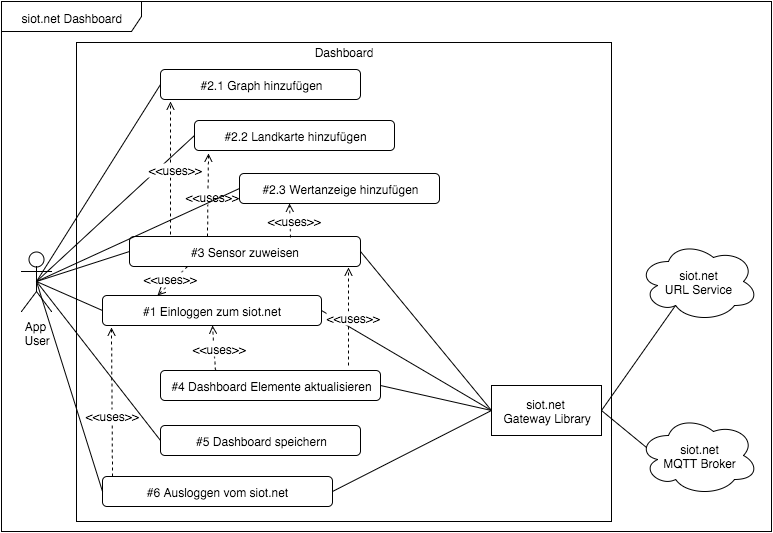
\includegraphics[scale=0.65]{98_Bilder/08_Requirements/UseCaseDashboard}
  \caption[Use Case siot.net Sensorcenter]{Das allgemeine Use Case Diagramm für das siot.net Dashboard}
\end{figure}
\newpage
\subsection{Funktionale Anforderungen und Anwendungsfallbeschreibungen}
\subsubsection{Anwendungsfall \#1}
Dieser Anwendungfall \#1 ist Deckungsgleich mit dessen im Kapitel 7.2.3, dem Anwendungsfall \#1.1. Das Login verfahren wird in beiden Applikationen identisch behandelt. Das Dashboard soll nur auf grösseren Android Geräten zur Verfügung stehen. Auf einem kleinen Display, der Wearable Devices, wäre die Darstellung der Informationen nicht übersichtlich.

\subsubsection{Anwendungsfall \#2}
\begin{table}[H]
\centering
\begin{tabular}{|>{\columncolor[gray]{0.8}}l|p{11.5cm}|}
\hline
\textbf{Nr. und Name:}                  & \#2.1 Graph, \#2.2 Landkarte und \#2.3 Wertanzeige hinzufügen. \\ \hline
\textbf{Szenario:}                      & Ein Anzeigeelement dem Dashboard hinzufügen. \\ \hline
\textbf{Kurzbeschreibung:}              & Der Applikation sollen wärend dem Betrieb, neue Objekte hinzugefügt werden können um Informationen anzuzeigen. \\ \hline
\textbf{Beteiligt Akteure:}             & App User. \\ \hline
\textbf{Auslöser und Vorbedingung:}     & User wählt ein neues Element aus. \\ \hline
\textbf{Ergebnisse und Nachbedingung:}  & Das ausgesuchte Anzeigeobjekt ist auf dem App sichtbar. \\ \hline
\end{tabular}
\caption{siot.net Dashboard: Übersicht Anwendungsfall \#2}
\end{table}
\textbf{Ablauf \#2:}
\begin{table}[H]
\centering
\begin{tabular}{|>{\columncolor[gray]{0.8}}p{1.3cm}|p{1.7cm}|p{13.2cm}|}
\hline
\textbf{2-1}  & App User  & Wählt einen Graph, Landkarte oder Freitext Wertanzeige aus. \\ \hline
\textbf{2-2}  & sDB       & Generiert das neue GUI Element und eine leere Auswahlliste. \\ \hline
\textbf{2-3}  & sDB       & Zeigt beide Objekte an. \\ \hline
\end{tabular}
\caption{siot.net Dashboard: Chronologischer Ablauf von Anwendungsfall \#2}
\end{table}
\textbf{Ausnahmen und Varianten \#2:}
\begin{table}[H]
\centering
\begin{tabular}{|>{\columncolor[gray]{0.8}}p{1.3cm}|p{1.7cm}|p{13.2cm}|}
\hline
\textbf{2-2.1}   & sDB    & Variante: Dem siot.net Dashboard sind bereits die Sensoren vom IoT Center bekannt, Auswahlliste kann bereits befüllt werden. \\ \hline
\end{tabular}
\caption{siot.net Dashboard: Ausnahmen und Varianten von Anwendungsfall \#2}
\end{table}

\subsubsection{Anwendungsfall \#3}
\begin{table}[H]
\centering
\begin{tabular}{|>{\columncolor[gray]{0.8}}l|p{11.5cm}|}
\hline
\textbf{Nr. und Name:}                  & \#3 Sensor zuweisen. \\ \hline
\textbf{Szenario:}                      & Einer sichtbaren Informationsanzeige einen dazugehörigen Sensor zuweisen. \\ \hline
\textbf{Kurzbeschreibung:}              & Die im Anwendungsfall \#2 generierte Auswahlliste soll mit passenden Sensoren gefüllt werden. Die Daten eines ausgewählten Sensors sollen auf der Anzeige dargestellt werden. \\ \hline
\textbf{Beteiligt Akteure:}             & App User, siot.net Gateway Library, siot.net MQTT Broker. \\ \hline
\textbf{Auslöser und Vorbedingung:}     & Neues Anzeigelement wurde erzeugt, User will ein Sensor dazu referenzieren. \\ \hline
\textbf{Ergebnisse und Nachbedingung:}  & Daten des ausgewählten Sensors werden auf dem Graph, der Landkarte oder der Wertanzeige dargestellt. \\ \hline
\end{tabular}
\caption{siot.net Dashboard: Übersicht Anwendungsfall \#3}
\end{table}
\textbf{Ablauf \#3:}
\begin{table}[H]
\centering
\begin{tabular}{|>{\columncolor[gray]{0.8}}p{1.3cm}|p{1.7cm}|p{13.2cm}|}
\hline
\textbf{3-1}  & App User  & Wählt eine Auswahlliste eines Anzeigeobjekt. \\ \hline
\textbf{3-2}  & sDB       & Verlangt von der siot.net Gateway Library alle vorhanden Sensoren mit passendem Typ. \\ \hline
\textbf{3-3}  & sDB       & Zeigt die verfügbaren Sensoren an. \\ \hline
\textbf{3-4}  & App User  & Wählt einen Sensor an. \\ \hline
\textbf{3-5}  & sDB       & Abonniert die Informationen bei der siot.net Gateway Library. \\ \hline
\textbf{3-6}  & sDB       & Anzeige wird mit den Daten dargestellt und synchronisiert. \\ \hline
\end{tabular}
\caption{siot.net Dashboard: Chronologischer Ablauf von Anwendungsfall \#3}
\end{table}
\textbf{Ausnahmen und Varianten \#3:}
\begin{table}[H]
\centering
\begin{tabular}{|>{\columncolor[gray]{0.8}}p{1.3cm}|p{1.7cm}|p{13.2cm}|}
\hline
\textbf{3-2.1}   & sDB    & Ausnahme: Keine Sensoren vorhanden, keine Aktion möglich, Auswahlliste bleibt leer. \\ \hline
\textbf{3-6.1}   & sDB    & Ausnahme: Keine Sensorendaten vorhanden, Anzeige wird erst angereichert wenn Daten eintreffen. \\ \hline
\end{tabular}
\caption{siot.net Dashboard: Ausnahmen und Varianten von  Anwendungsfall \#3}
\end{table}

\subsubsection{Anwendungsfall \#4}
\begin{table}[H]
\centering
\begin{tabular}{|>{\columncolor[gray]{0.8}}l|p{11.5cm}|}
\hline
\textbf{Nr. und Name:}                  & \#4 Dashboard Elemente aktualisieren. \\ \hline
\textbf{Szenario:}                      & Neu verfügbare Daten den Anzeigeobjekte zur Verfügung stellen. \\ \hline
\textbf{Kurzbeschreibung:}              & Die im Anwendungsfall \#3 abonnierte Daten müssen verarbeitet werden. Ein klassisches Model-View-Controller Pattern kommt hier zum Einsatz. \\ \hline
\textbf{Beteiligt Akteure:}             & siot.net Gateway Library, siot.net MQTT Broker. \\ \hline
\textbf{Auslöser und Vorbedingung:}     & siot.net Gateway Library empfängt neue MQTT Message und notifiziert das Dashboard. \\ \hline
\textbf{Ergebnisse und Nachbedingung:}  & Graph, der Landkarte oder der Wertanzeige wird aktualisiert. \\ \hline
\end{tabular}
\caption{siot.net Dashboard: Übersicht Anwendungsfall \#4}
\end{table}
\textbf{Ablauf \#4:}
\begin{table}[H]
\centering
\begin{tabular}{|>{\columncolor[gray]{0.8}}p{1.3cm}|p{1.7cm}|p{13.2cm}|}
\hline
\textbf{4-1}  & sDB       & Erhält die Benachrichtigung von der siot.net Gateway Library, dass neue Daten vorhanden sind. \\ \hline
\textbf{4-2}  & sDB       & Analysiert die Daten. \\ \hline
\textbf{4-3}  & sDB       & Aktualisiert die zu den Informationen gehörigen Anzeigen. \\ \hline
\end{tabular}
\caption{siot.net Dashboard: Chronologischer Ablauf von Anwendungsfall \#4}
\end{table}
\textbf{Ausnahmen und Varianten \#4:}
\begin{table}[H]
\centering
\begin{tabular}{|>{\columncolor[gray]{0.8}}p{1.3cm}|p{1.7cm}|p{13.2cm}|}
\hline
\textbf{3-2.1}   & sDB    & Ausnahme: Keine Daten welche relevant sind, keine Aktion nötig. \\ \hline
\end{tabular}
\caption{siot.net Dashboard: Ausnahmen und Varianten von  Anwendungsfall \#4}
\end{table}

\subsubsection{Anwendungsfall \#5}
\begin{table}[H]
\centering
\begin{tabular}{|>{\columncolor[gray]{0.8}}l|p{11.5cm}|}
\hline
\textbf{Nr. und Name:}                  & \#5 Dashboard speichern. \\ \hline
\textbf{Szenario:}                      & Das erstellt Dashboard speichern. \\ \hline
\textbf{Kurzbeschreibung:}              & Speichern des Dashboardes um es ein anderes Mal wieder zu verwenden oder auch anderen Usern im gleichen IoT Center bereit zu stellen. \\ \hline
\textbf{Beteiligt Akteure:}             & App User. \\ \hline
\textbf{Auslöser und Vorbedingung:}     & User drückt "`Dashboard speichern"' Taste. \\ \hline
\textbf{Ergebnisse und Nachbedingung:}  & Dashboard kann in einer Datei persistiert werden. \\ \hline
\end{tabular}
\caption{siot.net Dashboard: Übersicht Anwendungsfall \#5}
\end{table}
\textbf{Ablauf \#5:}
\begin{table}[H]
\centering
\begin{tabular}{|>{\columncolor[gray]{0.8}}p{1.3cm}|p{1.7cm}|p{13.2cm}|}
\hline
\textbf{5-1}  & App User  & Löst die Aktion aus durch betätigen des "`Dashboard speichern"' Knopfes. \\ \hline
\textbf{5-2}  & sDB       & Struktur und Zuordnungen werden in eine Datei auf dem Gerät niedergeschrieben. \\ \hline
\textbf{5-3}  & sDB       & User erhält Bestätigung. \\ \hline
\end{tabular}
\caption{siot.net Dashboard: Chronologischer Ablauf von Anwendungsfall \#5}
\end{table}
\textbf{Ausnahmen und Varianten \#5:}
\begin{table}[H]
\centering
\begin{tabular}{|>{\columncolor[gray]{0.8}}p{1.3cm}|p{1.7cm}|p{13.2cm}|}
\hline
\textbf{5-2.1}   & sDB    & Ausnahme: Datei kann nicht geschrieben werden, User benachrichtigen. \\ \hline
\end{tabular}
\caption{siot.net Dashboard: Ausnahmen und Varianten von  Anwendungsfall \#5}
\end{table}

\subsubsection{Anwendungsfall \#6}
\begin{table}[H]
\centering
\begin{tabular}{|>{\columncolor[gray]{0.8}}l|p{11.5cm}|}
\hline
\textbf{Nr. und Name:}                  & \#6 Ausloggen vom siot.net. \\ \hline
\textbf{Szenario:}                      & Löst die Verbindung zu der IoT Cloud auf. \\ \hline
\textbf{Kurzbeschreibung:}              & Dieser Schritt erlaubt eine saubere Abmeldung vom Netzwerk. Hier wird der Impuls der siot.net Gateway Library gegeben um alle Verbindungen Sauber zu trennen. \\ \hline
\textbf{Beteiligt Akteure:}             & App User, siot.net Gateway Library. \\ \hline
\textbf{Auslöser und Vorbedingung:}     & "`Abmelden"' Schaltfläche wird aktiviert. \\ \hline
\textbf{Ergebnisse und Nachbedingung:}  & Dashboard erfolgreich vom siot.net abgemeldet. \\ \hline
\end{tabular}
\caption{siot.net Dashboard: Übersicht Anwendungsfall \#6}
\end{table}
\textbf{Ablauf \#5:}
\begin{table}[H]
\centering
\begin{tabular}{|>{\columncolor[gray]{0.8}}p{1.3cm}|p{1.7cm}|p{13.2cm}|}
\hline
\textbf{5-1}  & App User  & Abmelden wird ausgeführt. \\ \hline
\textbf{5-2}  & sDB       & Meldet dem siot.net Gateway zum trennen der Verbindungen. \\ \hline
\textbf{5-3}  & sDB       & Login Bildschirm wird angezeigt. \\ \hline
\end{tabular}
\caption{siot.net Dashboard: Chronologischer Ablauf von Anwendungsfall \#6}
\end{table}
\textbf{Ausnahmen und Varianten \#6:}
\begin{table}[H]
\centering
\begin{tabular}{|>{\columncolor[gray]{0.8}}p{1.3cm}|p{1.7cm}|p{13.2cm}|}
\hline
\textbf{-}           & -    & Keine Ausnahmen und Varianten \\ \hline
\end{tabular}
\caption{siot.net Dashboard: Ausnahmen und Varianten von  Anwendungsfall \#6}
\end{table}

\subsection{Nicht-funktionale Anforderungen}
\textbf{Produktanforderungen:}
\begin{table}[H]
\centering
\begin{tabular}{|>{\columncolor[gray]{0.8}}p{5cm}|p{11.5cm}|}
\hline
\textbf{Benutzbarkeitsanforderungen}    & Die Applikation muss mit einem Android Smartphone funktionstüchtig sein. \\ \hline
\textbf{Effizienzanforderungen}         & Die Anwendung muss für aller Art Smartphone benutzer bedienbar sein. \\ \hline
\textbf{Zuverlässigkeitsanforderungen}  & Graphen, Landkarten und Werteanzeigen sollten möglichst flüssig angezeigt und aktualisiert werden. \\ \hline
\textbf{Portierbarkeitsanforderungen}   & Speichern eins Dashboards soll möglichst in einer generischen Struktur geschehen. In einem weiteren Release wir in betracht gezogen, dass Dashboards portierbar sind, das heisst sie können auch im siot.net IoT Center gespeichert werden.\\ \hline
\textbf{Performanceanforderung}         & Die Anzeige muss flüssig reagieren um die Graphen brauchbar zu visualisieren. Es braucht eine Internetverbindung, um Sensorinformationen zu empfangen. Da die Datenpakete sehr klein sind (<1KB), ist keine sehr grosse Bandbreite notwendig. \\ \hline
\end{tabular}
\caption{siot.net Dashboard: Nicht-funktionale Produktanforderungen}
\end{table}


% Main part - Part VIII
%---------------------------------------------------------------------------
\onecolumn
\include{09_Softwaredesign/01_Softwaredesign}

%---------------------------------------------------------------------------

%---------------------------------------------------------------------------

% Index
%---------------------------------------------------------------------------
%\cleardoublepage
%\phantomsection
%\addcontentsline{toc}{chapter}{Stichwortverzeichnis}
%\renewcommand{\indexname}{Stichwortverzeichnis}
%\printindex
%---------------------------------------------------------------------------

%---------------------------------------------------------------------------
\end{document}
